\documentclass[12pt,titlepage]{article}
\usepackage[margin=1in]{geometry}
\usepackage{parskip}
% \usepackage{float}
\usepackage{amsthm}
\usepackage{amsmath,amsfonts,graphicx}
\usepackage{floatrow}
\usepackage{tcolorbox}
\usepackage{dsfont}
\usepackage{xcolor}
\usepackage{framed}
\usepackage{hyperref}
\usepackage{titlesec}

\usepackage{algo,tikz,url,amssymb,epsfig,color,xspace}
% for making graphs
\usetikzlibrary{arrows}
\usetikzlibrary[patterns]
\usepackage{mathrsfs}
\usepackage{pgfplots}
\pgfplotsset{compat=1.15}

% pair symbols
\usepackage{mathtools}
\DeclarePairedDelimiter\ceil{\lceil}{\rceil}
\DeclarePairedDelimiter\floor{\lfloor}{\rfloor}

\DeclareMathOperator\cis{cis}
\DeclareMathOperator\Arg{Arg}
\DeclareMathOperator\Log{Log}

% algorithms
\usepackage[linesnumbered,ruled,vlined]{algorithm2e}
\newcommand\mycommfont[1]{\footnotesize\ttfamily\textcolor{blue}{#1}}
\SetCommentSty{mycommfont}

\SetKwInput{KwInput}{Input}                % Set the Input
\SetKwInput{KwOutput}{Output}              % set the Output

\usepackage{fancyhdr}
\pagestyle{fancy}
\fancyhf{}
\renewcommand{\footrulewidth}{0.4pt}

% \setlength{\parindent}{4ex}
\titleformat{\section}{\normalfont\Large\bfseries}{Chapter \thesection}{1em}{}
% \renewcommand{\thesection}{Chapter \arabic{section}}

\lhead{AMATH 332 / PMATH 332}
\chead{Spring 2021}
\rhead{Course Notes}
% \rfoot{Page \thepage\ of \pageref*{LastPage}}
\rfoot{Page \thepage}
\cfoot{}
\lfoot{\copyright Haochen Wu 2021}


\newtheorem{prototheorem}{Theorem}[section]
\newenvironment{theorem}
{\colorlet{shadecolor}{orange!15}\begin{shaded}\begin{prototheorem}\normalfont}{\end{prototheorem}\end{shaded}}

\newtheorem{protolemma}[prototheorem]{Lemma}
\newenvironment{lemma}
{\colorlet{shadecolor}{violet!15}\begin{shaded}\begin{protolemma}\normalfont}{\end{protolemma}\end{shaded}}

\newtheorem{protocorollary}[prototheorem]{Corollary}
\newenvironment{corollary}
{\colorlet{shadecolor}{yellow!15}\begin{shaded}\begin{protocorollary}\normalfont}{\end{protocorollary}\end{shaded}}

\newtheorem{protonotation}[prototheorem]{Proposition}
\newenvironment{proposition}
{\colorlet{shadecolor}{green!15}\begin{shaded}\begin{protonotation}\normalfont}{\end{protonotation}\end{shaded}}

\newtheorem{protoexample}[prototheorem]{Example}
\newenvironment{example}
{\colorlet{shadecolor}{red!15}\begin{shaded}\begin{protoexample}\normalfont}{\end{protoexample}\end{shaded}}

\newtheorem{protodefinition}[prototheorem]{Definition}
\newenvironment{definition}
{\colorlet{shadecolor}{cyan!15}\begin{shaded}\begin{protodefinition}\normalfont}{\end{protodefinition}\end{shaded}}

\newtheorem{protoproof}[prototheorem]{Proof}
\renewenvironment{proof}
{\colorlet{shadecolor}{blue!15}\begin{shaded}\begin{protoproof}\normalfont}{\qed\end{protoproof}\end{shaded}}

\let\stdsection\section
\renewcommand\section{\clearpage\stdsection}

\usepackage{hyperref}
\hypersetup{
  linktoc=all
}

\begin{document}
\begin{titlepage}
	\vspace*{\fill}
	\centering
		
	\textbf{\Huge AMATH / PMATH 332 Course Notes} \\ [0.4em]
	\textbf{\Large Applied Complex Analysis} \\ [1em]
	\textbf{\Large Haochen Wu} \\ [1em]
	\textbf{\large University of Waterloo} \\
	\textbf{\large Spring 2021} \\
	\vspace*{\fill}
\end{titlepage}

\newpage 

\pagenumbering{roman}

\tableofcontents
\newpage
% \listofalgorithms
% \newpage
% \listoffigures
% \newpage

\pagenumbering{arabic}

\section{Complex Numbers}
\subsection{Intro, Properties of Complex Numbers}
Intro: \begin{itemize}
	\item What it's about: \underline{not} like real analysis; some of intro to calculus on $\mathbb{C}$
	\item Goal: extend calculus on $\mathbb{R}$ to $\mathbb{C}$ - many results become \underline{simpler}! (more complete picture here)
	\item Can be used to solve some $\mathbb{R}$ problems. 
\end{itemize}

The Fundamentals: \begin{itemize}
	\item Basic idea: define solutions to $x^2 + 1 = 0$
	\item Early Mathematicians: $x = \pm \sqrt{-1}$. For $\sqrt{-1}$, should we call it $i$? 
	\item Note: ``$\sqrt{\;\;\;}$'' always denotes \underline{positive} root, e.g. $\sqrt{4} = 2$
	\item Problem: \begin{align*}
		\sqrt{-1}\sqrt{-1} &= -1 \;\;\;\text{ by definition of }\sqrt{\;\;\;}\\
		\sqrt{-1}\sqrt{-1} &= \sqrt{(-1)(-1)} = \sqrt{1} = 1 \;\;\;\text{ since } \sqrt{ab} = \sqrt{a}\sqrt{b}
	\end{align*}
	\item Fix: intepret ``$\sqrt{\;\;\;}$'' differently for complex numbers - it must be multivalued, and define the imaginary unit $i$ by $i^2 = 1$
\end{itemize}
\begin{definition}
	\underline{\textbf{Complex number}}: $$z = \underbrace{a}_{\text{``real part''} \;\; Re(z)} + i\underbrace{b}_{\text{``imaginary part''} \;\; Im(z) \text{ which is real!}} \;\; \text{ where } a, b \in \mathbb{R}$$
	$\mathbb{C} = $ set of complex numbers. Note that $\mathbb{R} \subset \mathbb{C}$
\end{definition}
\begin{definition}
	Let $z = a + bi$, and $w = c + di$. Then: \begin{itemize}
		\item $z = w$ if and only if $a=c$ and $b=d$
		\item $z+w = (a+bi) + (c+di) = a+c+(b+d)i$
		\item $z-w = z+ (-w) = (a+bi)+(-c-di) = a-c+(b-d)i$
		\item $zw = (a+bi)(c+di) = ac+bdi^2+adi+bci = ac-bd+(ad+bc)i$
		\item $\dfrac{z}{w} = \dfrac{a+bi}{c+di} \cdot \dfrac{c-di}{c-di} = \dfrac{ac+bd}{c^2+d^2} + i \cdot \dfrac{bc-ad}{c^2+d^2}$
	\end{itemize}
\end{definition}
\begin{example}
	$$\frac{2+i}{1+2i} = \frac{2+i}{1+2i} \cdot \frac{1-2i}{1-2i} = \frac{4}{5} - \frac{3}{5}i$$
	$$\frac{1}{i} = \frac{1}{i} \cdot \frac{-i}{-i} = \frac{-i}{-i^2} = -i$$
\end{example}
\begin{theorem}
	$z+w = w + z$, $k(z+w) = kz + kw$ apply as usual. $zw = wz$
\end{theorem}
Note: We can't classify complex numbers as ``positive'' or ``negative'', and can't use inequalities, e.g. $z > w$ doesn't make sense. 
\begin{definition}
	\textbf{\underline{Conjugate}} of $z = a+bi$ is $$\overline{z} = a-bi$$
	(Sometimes written as $z^*$ as well)
\end{definition}
\begin{proposition}
	The following rules apply: 
	\begin{enumerate}
		\item $\overline{\overline{z}} = z$
		\item $\overline{z \pm w} = \overline{z} \pm \overline{w}$
		\item $\overline{zw} = \overline{z} \;\overline{w}$ and $\overline{\bigg(\dfrac{z}{w}\bigg)} = \dfrac{(\overline{z})}{(\overline{w})}$
		\item $z + \overline{z} = 2Re(z) \;\; \Rightarrow \;\; Re(z) = \frac{1}{2}(z + \overline{z})$
		\item $z - \overline{z} = 2iIm(z) \;\; \Rightarrow \;\; Im(z) = \frac{1}{2i}(z - \overline{z})$
		\item $z\overline{z} = a^2+b^2$ which is real!
	\end{enumerate}
\end{proposition}
\begin{center}
	\begin{tikzpicture}
		\begin{axis}[
			x=1cm,y=1cm,
			axis lines=middle,
			grid style=dashed,
			xmin=-3,
			xmax=6,
			ymin=-2,
			ymax=6,
			xtick=\empty,
			ytick=\empty,]
			\draw [->,line width=0.8pt] (0,0) -- (0.49,3.04);
			\draw [->,line width=0.8pt] (0,0) -- (4,2);
			\draw [->,line width=0.8pt] (0,0) -- (4.49,5.04);
			\draw [->,line width=0.8pt,dash pattern=on 1pt off 1pt,color=red] (0.49,3.04) -- (4.49,5.04);
			\draw [->,line width=0.8pt,dash pattern=on 1pt off 1pt,color=red] (4,2) -- (4.49,5.04);
			\begin{scriptsize}
				\draw [fill=black] (0,0) circle (1.5pt);
				\draw [fill=black] (0.49,3.04) circle (1.5pt);
				\draw [fill=black] (4,2) circle (1.5pt);
				\draw[color=black] (0.74,2) node {$z_2$};
				\draw[color=black] (2.46,1.06) node {$z_1$};
				\draw[color=black] (2.58,2.54) node {$z_1+z_2$};
				\draw [fill=black] (4.49,5.04) circle (1.5pt);
			\end{scriptsize}
		\end{axis}
	\end{tikzpicture}\\
\end{center}

\subsection{The Complex Plane, Polar form}
\begin{center}
	\begin{tikzpicture}
		\draw [->,line width=2pt] (0,-2) -- (0,3);
		\draw [->,line width=2pt] (-3,0) -- (4,0);
		\draw (0.3,3.86) node[anchor=north west] {Im$(z)$};
		\draw (4.28,-0.02) node[anchor=north west] {Re$(z)$};
		\draw (2.9,-0.02) node[anchor=north west] {$a$};
		\draw (-0.84,2.64) node[anchor=north west] {$b$};
		\draw (3.66,2.62) node[anchor=north west] {$z=a+bi$};
		\begin{scriptsize}
			\draw [fill=black] (0,2) circle (1.5pt);
			\draw [fill=black] (3,0) circle (1.5pt);
			\draw [fill=black] (3,2) circle (1.5pt);
		\end{scriptsize}
	\end{tikzpicture}
	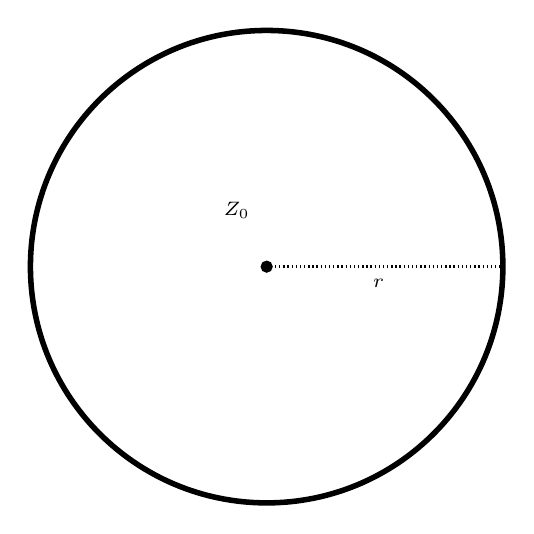
\begin{tikzpicture}
		\draw [line width=2pt] (0,0) circle (3cm);
		\draw [line width=1pt,dash pattern=on 0.5pt off 1pt] (0,0)-- (3,0);
		\begin{scriptsize}
			\draw [fill=black] (0,0) circle (2pt);
			\draw[color=black] (-0.38,0.71) node {$Z_0$};
			\draw[color=black] (1.42,-0.21) node {$r$};
		\end{scriptsize}
	\end{tikzpicture}
\end{center}
\begin{definition}
	The \textbf{\underline{modulus}} of $z = a+bi$ is $|z| = \sqrt{a^2+b^2}$

	The \underline{\textbf{distance}} between two numbers $z$ and $w$ is $|z-w|$
\end{definition}
Notes: \begin{itemize}
	\item $|z| \geq 0$ and is real
	\item $z\overline{z} = a^2+b^2 = |z|^2$
	\item $|z-z_0| = r$ describes a circule of radius $r$ centered at $z_0$
\end{itemize}
\begin{example}
	Sketch the sets: \begin{enumerate}
		\item $|z| < 3$
		\begin{center}
			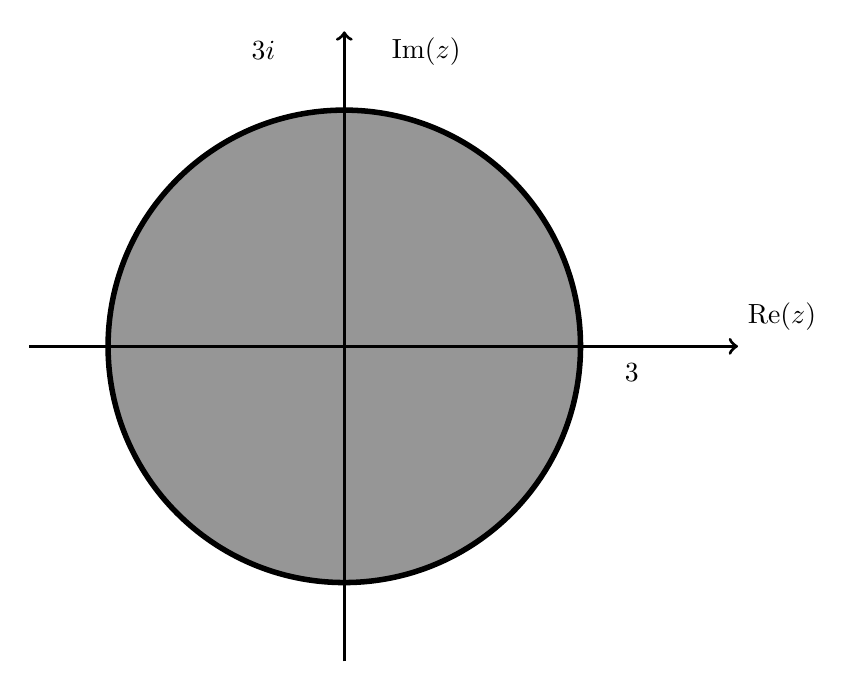
\begin{tikzpicture}
				\draw [line width=2pt,fill=black,fill opacity=0.41] (0,0) circle (3cm);
				\draw [->,line width=1.2pt] (0,-4) -- (0,4);
				\draw [->,line width=1.2pt] (-4,0) -- (5,0);
				\draw (-1.3,4) node[anchor=north west] {$3i$};
				\draw (3.44,-0.1) node[anchor=north west] {$3$};
				\draw (5,0.68) node[anchor=north west] {Re$(z)$};
				\draw (0.48,4.04) node[anchor=north west] {Im$(z)$};
			\end{tikzpicture}
		\end{center}
		\item $|z| = Im(z)$. Let $z = a+ib$. So, $\sqrt{a^2+b^2} = b$, which gives $a^2+b^2 = b^2$, so $a = 0, b \geq 0$
		\begin{center}
			\begin{tikzpicture}
				\begin{axis}[
					x=1cm,y=1cm,
					axis lines=middle,
					xmin=-5,
					xmax=5,
					ymin=-1,
					ymax=5,
					xtick=\empty,
					ytick=\empty,]
				\end{axis}
				\draw [line width=3pt] (5,6)--(5,1);
				\draw (5.2,6) node[anchor=north west] {Im$(z)$};
				\draw (10,1.5) node[anchor=north west] {Re$(z)$};
			\end{tikzpicture}
		\end{center}
		\item $|z-1| = |z+i|$. So 
		\begin{align*}
		\sqrt{(a-1)^2+b^2} &= \sqrt{a^2+(b+1)^2} \\
		(a-1)^2+b^2 &= a^2+(b+1)^2\\
		a^2 - 2a+1+b^2 &= a^2+b^2+2b+1\\
		b &= -a
		\end{align*}
		This is the set of points that are equidistant from $z = 1$ and $z= -i$
		\begin{center}
			\begin{tikzpicture}
				\begin{axis}[
					x=1cm,y=1cm,
					axis lines=middle,
					xmin=-5,
					xmax=5,
					ymin=-5,
					ymax=5,
					xtick=\empty,
					ytick=\empty,]
				\end{axis}
			\draw [line width=2pt] (2,8)--(8,2);
			\draw (5.2,10) node[anchor=north west] {Im$(z)$};
			\draw (10,5.5) node[anchor=north west] {Re$(z)$};
			\end{tikzpicture}
		\end{center}
	\end{enumerate}
\end{example}

We will often use $z = x+yi$, so we are in the $xy$-plane, still not called $\mathbb{R}^2$ though. 

Useful inequalities: $$|z_1 + z_2| \leq |z_1| + |z_2|$$
This is known as ``Triangle Inequality''. This also extends to $$|z_1 = z_2 + \cdots + z_n| \leq |z_1| + \cdots + |z_n|$$

\begin{corollary}
	$$|z_1 + z_2| \geq \bigg||z_1| - |z_2|\bigg|$$
\end{corollary}
\begin{proof}
	\begin{align*}
		|z_1| &= |z_1 + (z_2-z_2)|\\
		&=|(z_1 + z_2)+(-z_2)|\\
		&\leq |z_1 + z_2| + |z_2|
	\end{align*}
	\begin{align*}
		|z_2| &= |z_2 + (z_1-z_1)|\\
		&=|(z_1 + z_2)+(-z_1)|\\
		&\leq |z_1 + z_2| + |z_1|
	\end{align*}
	So $|z_1+z_2| \geq |z_1| - |z_2|$ and $|z_2| - |z_1|$. So $$|z_1 + z_2| \geq \bigg||z_1| - |z_2|\bigg|$$
\end{proof}

\begin{definition}
	\textbf{\underline{Polar Form}}
	\begin{tcolorbox}[hbox, before=\par\smallskip\centering]
		$x = r\cos \theta$, $y = r\sin \theta$
	\end{tcolorbox}
	So, \begin{align*}
		z&= r\cos \theta + ir\sin\theta\\
		&=r(\cos \theta + i\sin\theta)\\
		&=r \underbrace{\cis}_{\text{common abreviation}} \theta
	\end{align*}
	\begin{tcolorbox}[hbox, before=\par\smallskip\centering]
		$r = \sqrt{x^2+y^2}$, $\tan \theta = \dfrac{y}{x}$
	\end{tcolorbox}
	\begin{center}
		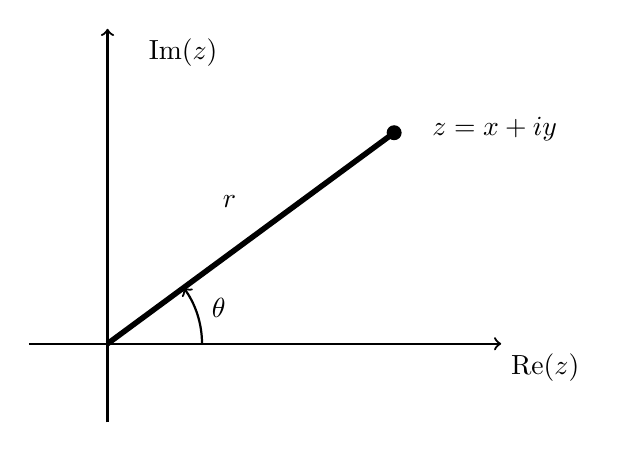
\begin{tikzpicture}
			\draw [->,line width=0.8pt] (-1,0) -- (5,0);
			\draw [->,line width=0.8pt] (0,-1) -- (0,4);
			\draw (0.4,4) node[anchor=north west] {Im$(z)$};
			\draw (5,0) node[anchor=north west] {Re$(z)$};
			\draw [line width=2pt] (0,0)-- (3.64,2.68);
			\draw [shift={(0,0)},->,line width=0.8pt] (0:1.2) arc (0:36.362868584929245:1.2);
			\draw (1.2,0.7) node[anchor=north west] {$\theta$};
			\draw (4,3) node[anchor=north west] {$z=x+iy$};
			\draw (1.34,2) node[anchor=north west] {$r$};
			\draw [fill=black] (3.64,2.68) circle (2.5pt);
			\end{tikzpicture}
	\end{center}
\end{definition}
Notes: \begin{itemize}
	\item This is not unique. e.g. $z = 2 = 2\cis 0 = 2\cis 2\pi = \cdots$, also $z = 0 = 0 \cis \theta$ for any $\theta$
	\item $\theta = \tan^{-1}(\dfrac{y}{x})[\pm 2k\pi]$ if $x > 0$, but must add $\pi$ if $x < 0$ - Recall principal values
\end{itemize}
\begin{example}
	Say we want to express $z = -1-i$ in polar form. 
	
	We compute $r = \sqrt{(-1)^2+(-1)^2} = \sqrt{2}$. $\tan \theta = \dfrac{-1}{-1} = 1$. Note that $\theta \neq \tan^{-1}(1) = \dfrac{\pi}{4}$, instead, $\theta = \dfrac{5\pi}{4}$. 

	So, $z = \sqrt{2}\cis \dfrac{5\pi}{4}$ or $\sqrt{2}\cis (\dfrac{5\pi}{4} + 2k\pi)$
	\begin{center}
		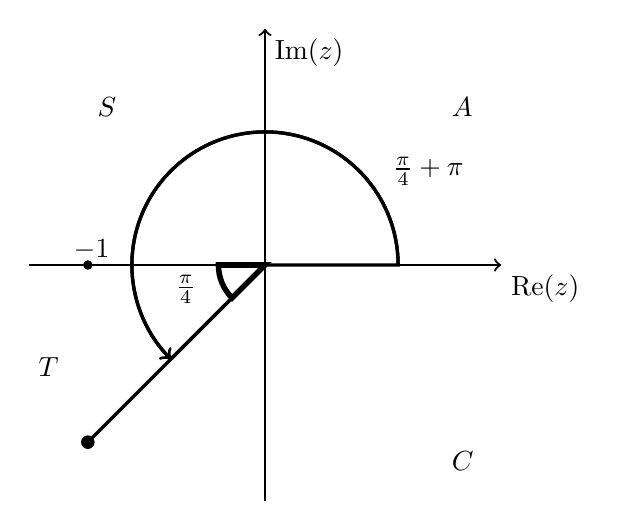
\begin{tikzpicture}[scale=1.5]
			\draw [->,line width=0.8pt] (-2,0) -- (2,0);
			\draw [->,line width=0.8pt] (0,-2) -- (0,2);
			\draw (0,2) node[anchor=north west] {Im$(z)$};
			\draw (2,0) node[anchor=north west] {Re$(z)$};
			\draw [fill=black] (-1.5,-1.5) circle (1.5pt);
			\draw [fill=black] (-1.5,0) circle (1pt);
			\draw (-1.7,0.3) node[anchor=north west] {$-1$};
			\draw [shift={(0,0)},line width=1.2pt] (0,0) -- (0:1.127026791712589) arc (0:225:1.127026791712589) -- cycle;
			\draw [shift={(0,0)},line width=2pt] (0,0) -- (180:0.39445937709940615) arc (180:225:0.39445937709940615) -- cycle;	
			\draw [line width=1.2pt] (0,0)-- (-1.5,-1.5);
			\draw [shift={(0,0)},->,line width=1.2pt] (0:1.127026791712589) arc (0:225:1.127026791712589);
			\draw (-0.84,0) node[anchor=north west] {$\frac{\pi}{4}$};
			\draw (1,1) node[anchor=north west] {$\frac{\pi}{4}+\pi$};
			\draw (1.5,1.5) node[anchor=north west] {$A$};
			\draw (-1.5,1.5) node[anchor=north west] {$S$};
			\draw (-2,-0.7) node[anchor=north west] {$T$};
			\draw (1.5,-1.5) node[anchor=north west] {$C$};
			\end{tikzpicture}
	\end{center}
\end{example}
Note: $$z = \underbrace{r}_{=\sqrt{x^2+y^2}, r = |z|, \text{``modulus''}}\cis \underbrace{\theta}_{\text{``argument'' of }z}$$
Also, ``$\arg z$'' = set of all possible values of $\theta$. ``$\Arg z$'' = principle values of $\theta$, usually in $(\pi, \pi]$

\begin{example}
	For $z = -1 + \sqrt{3}i$. $\Arg z = \dfrac{2\pi}{3}$, $\arg z = \dfrac{2\pi}{3} + 2k\pi, k \in \mathbb{Z}$

	Also, $|z| = 2$, so $-1 + \sqrt{3}i = 2\cis \dfrac{2\pi}{3}$
\end{example}

We sometimes think of $\arg z$ as a multivalued ``function'' of $z$. For a single-valued function, we could use $\Arg z$, but it has discontinuity on negative real axis. 
\begin{center}
	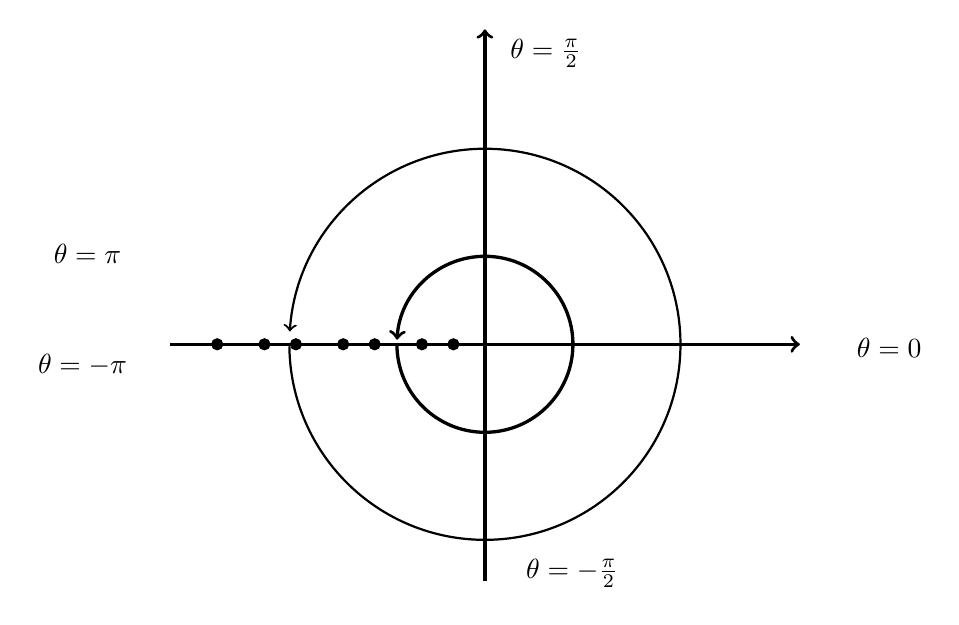
\begin{tikzpicture}[scale=2]
		\draw [->,line width=1.2pt] (0,-1.5) -- (0,2);
		\draw [->,line width=1.2pt] (-2,0) -- (2,0);
		
		\draw [shift={(0,0)},->,line width=1.2pt] (-180:0.558829190753239) arc (-180:177.02028294976014:0.558829190753239);
		\draw [shift={(0,0)},->,line width=0.8pt] (-179.42598203648794:1.241842646118309) arc (-179.42598203648794:176.2439591765568:1.241842646118309);
		\draw (2.3,0.1) node[anchor=north west] {$\theta=0$};
		\draw (0.1,2) node[anchor=north west] {$\theta=\frac{\pi}{2}$};
		\draw (0.2,-1.3) node[anchor=north west] {$\theta=-\frac{\pi}{2}$};
		\draw (-2.9,0) node[anchor=north west] {$\theta=-\pi$};
		\draw (-2.8,0.7) node[anchor=north west] {$\theta=\pi$};
		\begin{scriptsize}
			\draw [fill=black] (-0.2,0) circle (1pt);
			\draw [fill=black] (-0.4,0) circle (1pt);
			\draw [fill=black] (-0.7,0) circle (1pt);
			\draw [fill=black] (-0.9,0) circle (1pt);
			\draw [fill=black] (-1.2,0) circle (1pt);
			\draw [fill=black] (-1.4,0) circle (1pt);
			\draw [fill=black] (-1.7,0) circle (1pt);
		\end{scriptsize}
		\end{tikzpicture}
\end{center}

Another way: we can define $\Arg(z)$ to have range $[0, 2\pi)$. In general, $\Arg_{\theta_0}z$ has range $[\theta_0, \theta_0 + 2\pi)$, and usually we use $\Arg z = \Arg_{-\pi} z$
\begin{center}
	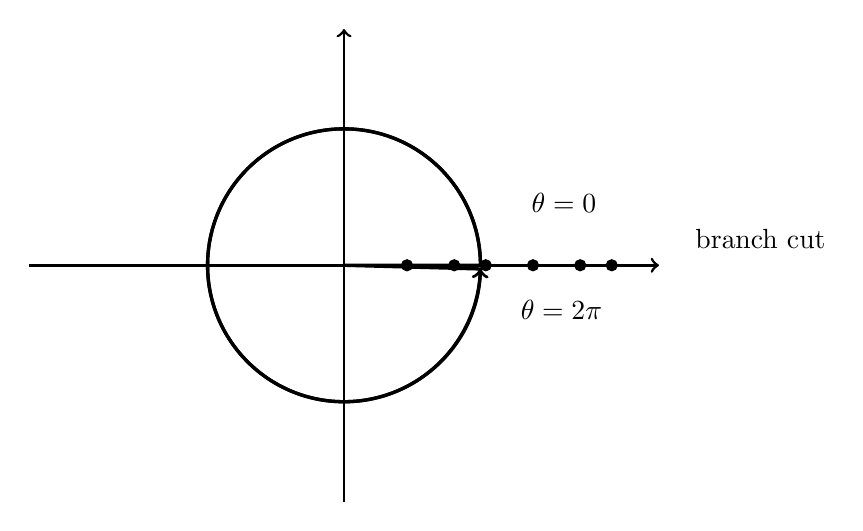
\begin{tikzpicture}[scale=2]
		\draw [shift={(0,0)},line width=1.2pt] (0,0) -- (0:0.8664438145013174) arc (0:358.45044092547164:0.8664438145013174) -- cycle;
		\draw [shift={(0,0)},->,line width=1.2pt] (0:0.8664438145013174) arc (0:358.45044092547164:0.8664438145013174);
		\draw (1.1296312880955108,0.5174728527862119) node[anchor=north west] {$\theta=0$};
		\draw [->,line width=1pt] (0,-1.5) -- (0,1.5);
		\draw [->,line width=1pt] (-2,0) -- (2,0);
		\draw (1.0603157829354055,-0.15835332252481515) node[anchor=north west] {$\theta=2\pi$};
		\draw (2.1693638654970915,0.2921974610158696) node[anchor=north west] {branch cut};
		\begin{scriptsize}
			\draw [fill=black] (0.4,0) circle (1pt);
			\draw [fill=black] (0.7,0) circle (1pt);
			\draw [fill=black] (0.9,0) circle (1pt);
			\draw [fill=black] (1.2,0) circle (1pt);
			\draw [fill=black] (1.5,0) circle (1pt);
			\draw [fill=black] (1.7,0) circle (1pt);
		\end{scriptsize}
	\end{tikzpicture}
\end{center}

\subsection{Complex Exponential, Powers and Roots}
Reading textbook Section 1.4, 1.5
\begin{definition}
	If $z = x+ iy$, then $e^z$ is defined to be the complex number $$e^z := e^x (\cos y + i\sin y)$$
\end{definition}
\begin{proposition}
	Euler's equation is formally consistent with the usual Taylor series expansions: \begin{align*}
		e^x &= 1 + x + \dfrac{x^2}{2!} + \dfrac{x^3}{3!} + \cdots\\
		\cos x &= 1 - \dfrac{x^2}{2!} + \dfrac{x^4}{4!} - \cdots\\
		\sin x &= x - \dfrac{x^3}{3!} + \dfrac{x^5}{5!} - \cdots
	\end{align*}
\end{proposition}
\begin{proof}
	Let's substitute $x = iy$ into the exponential series: \begin{align*}
		e^{iy} &= 1 + iy + \dfrac{(iy)^2}{2!} + \dfrac{(iy)^3}{3!} + \cdots\\
		&=(1-\dfrac{y^2}{2!} + \dfrac{y^4}{4!} - \cdots) + i(y-\dfrac{y^3}{3!} + \dfrac{y^5}{5!} - \cdots)\\
		&=\cos y + i\sin y
	\end{align*}
\end{proof}
As a result, we may introduce the standard polar representation $$z = r \cis \theta = r(\cos \theta + i \sin \theta) = re^{i\theta} = |z|e^{i \arg z}$$

Notice that $$e^{i0} = e^{2\pi i} = e^{-2\pi i} = e^{4\pi i} = e^{-4\pi i} = \cdots = 1$$
$$e^{(\pi / 2)i} = i \;\;\;\; e^{(-\pi/2) i}= -i \;\;\;\; e^{\pi i} = -1$$

Also notice that \begin{align*}
	\cos \theta &= Re(e^{i\theta}) = \dfrac{e^{i\theta} + e^{-i\theta}}{2} \\
	\sin \theta &= Im(e^{i\theta}) = \dfrac{e^{i\theta} - e^{-i\theta}}{2i} 
\end{align*}

Hence, $$z_1z_2 = (r_1e^{i\theta_1})(r_2e^{i\theta_2}) = (r_1r_2)e^{i(\theta_1+\theta_2)}$$
$$\dfrac{z_1}{z_2} = \dfrac{r_1e^{i\theta_1}}{r_2e^{i\theta_2}} = \dfrac{r_1}{r_2}e^{i(\theta_1-\theta_2)}$$
$$\overline{z} = re^{-i\theta}, \text{ given that }z = re^{i\theta}$$
\begin{example}
	Compute the following:
	\begin{enumerate}
		\item $(1+i)/(\sqrt{3}-i)$. 
		
		Notice that $1+i = \sqrt{2}\cis(\pi/4) = \sqrt{2}e^{i\pi/4}$, and $\sqrt{3}-i = 2\cis(-\pi /6) = 2e^{-i\pi/6}$. So, $$\dfrac{1+i}{\sqrt{3}-i} = \dfrac{\sqrt{2}e^{i\pi/4}}{2e^{-i\pi/6}} = \dfrac{\sqrt{2}}{2}e^{i5\pi/12}$$
		\item $(1+i)^{24}$
		
		We have $$(1+i)^{24} = (\sqrt{2}e^{i\pi/4})^{24} = (\sqrt{2})^{24}e^{i24\pi/4} = 2^{12}e^{i6\pi} = 2^{12}$$
	\end{enumerate}
\end{example}
\begin{theorem}
	$$(\cos \theta + i\sin \theta)^n = \cos n\theta + i \sin n\theta \;\;\;\; n = 1, 2, 3, ...$$
\end{theorem}
\begin{definition}
	There are exactly $m$ distinct $m$-th \underline{\textbf{roots of unity}}, denoted by $1^{1/m}$, and they are given by
	$$1^{1/m} = e^{i2k\pi/m} = \cos \dfrac{2k\pi}{m} + i\sin \dfrac{2k\pi}{m} \;\;\;\;(k = 0,1, 2, ..., m-1)$$

	Take $k = 1$ into the above equation, we can get $$\omega_m := e^{i2\pi/m} = \cos \dfrac{2\pi}{m} + i\sin \dfrac{2\pi}{m}$$
	So the complete set of roots can be displayed as$$\{1, \omega_m, \omega_m^2, \cdots, \omega_m^{m-1}\}$$
	Note that a number $w$ is said to be a \underline{\textbf{primitive}} $m$-th root of unity if $w^m = 1$ but $w^k \neq 1$ for $k = 1, 2, ..., m-1$. Clearly, $\omega_m$ is a primitive root. 
\end{definition}
\begin{theorem}
	$$1+\omega_m + \omega_m^2 + \cdots + \omega_m^{m-1} = 0$$
\end{theorem}
\begin{proof}
	Note that $$(\omega_m - 1) (1+\omega_m + \omega_m^2 + \cdots + \omega_m^{m-1}) = (\omega_m - 1) = 0$$
	Since $\omega_m \neq 1$, the result follows. 
\end{proof}
To obtain the $m$-th root of an arbitrary (non-zero) complex number $z = re^{i\theta}$, we can obtain the following generalized result. 
\begin{definition}
	The $m$-th distinct roots of $z$ are given by $$z^{1/m} = \sqrt[m]{|z|} e^{i (\theta + 2k\pi)/m}$$
\end{definition}
\begin{example}
	Find all the cube roots of $\sqrt{2} + i\sqrt{2}$

	The polar form for $\sqrt{2} + i\sqrt{2}$ is $$\sqrt{2} + i\sqrt{2} = 2e^{i\pi/4}$$
	Putting $|z|=2, \theta = \pi/4, m = 3$ into the above definition, we obtain $$(\sqrt{2} + i\sqrt{2})^{1/3} = \sqrt[3]{2}e^{i(\pi/12+2k\pi/3)}, \;\;\;\;(k = 0, 1, 2)$$
	Hence, the three cube roots of $\sqrt{2} + i\sqrt{2}$ are: \begin{itemize}
		\item $\sqrt[3]{2} (\cos \pi/12 + i\sin \pi/12)$
		\item $\sqrt[3]{2} (\cos 3\pi/4 + i\sin 3\pi/4)$
		\item $\sqrt[3]{2} (\cos 17\pi/12 + i\sin 17\pi/12)$
	\end{itemize}
\end{example}
\subsection{Application to Electrical Circuits}
A typical electrical circuits is like the following: 

\begin{figure}[h!]
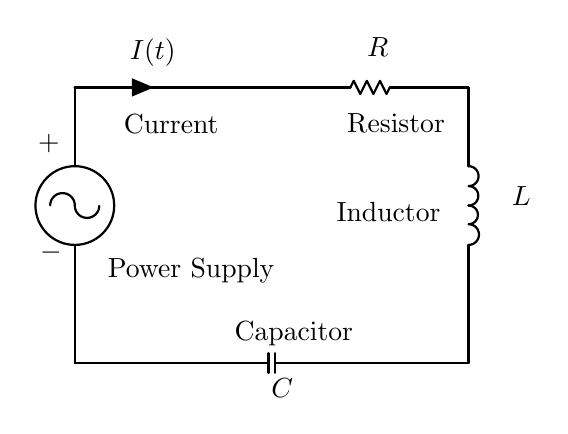
\begin{tikzpicture}[line cap=round,line join=round,>=triangle 45,x=1cm,y=1cm]
	\draw [line width=0.8pt] (0.5,-1.5)-- (-1.9583333333333333,-1.5);
	\draw [line width=0.8pt] (-4.5,-1.5)-- (-2.0416666666666665,-1.5);
	\draw [line width=0.8pt] (-1.9583333333333333,-1.625)-- (-1.9583333333333333,-1.375);
	\draw [line width=0.8pt] (-2.0416666666666665,-1.625)-- (-2.0416666666666665,-1.375);
	\draw [line width=0.8pt] (-0.5,2)-- (-0.5416666666666666,1.9166666666666667);
	\draw [line width=0.8pt] (-0.5416666666666666,1.9166666666666667)-- (-0.625,2.0833333333333335);
	\draw [line width=0.8pt] (-0.625,2.0833333333333335)-- (-0.7083333333333334,1.9166666666666667);
	\draw [line width=0.8pt] (-0.7083333333333334,1.9166666666666667)-- (-0.7916666666666666,2.0833333333333335);
	\draw [line width=0.8pt] (-0.7916666666666666,2.0833333333333335)-- (-0.875,1.9166666666666667);
	\draw [line width=0.8pt] (-0.875,1.9166666666666667)-- (-0.9583333333333334,2.0833333333333335);
	\draw [line width=0.8pt] (-0.9583333333333334,2.0833333333333335)-- (-1,2);
	\draw [line width=0.8pt] (0.5,2)-- (-0.5,2);
	\draw [line width=0.8pt] (-1,2)-- (-2,2);
	\draw [line width=0.8pt] (-4.5,2)-- (-2,2);
	\draw [line width=0.8pt] (-4.5,0.5) circle (0.5cm);
	\draw [line width=0.8pt] (-4.5,2)-- (-4.5,1);
	\draw [line width=0.8pt] (-4.5,0)-- (-4.5,-1.5);
	\draw [->,line width=0.8pt] (-4.5,2) -- (-3.5,2);
	\draw [shift={(-4.656590387120971,0.5012436450386237)},line width=0.8pt]  plot[domain=-0.007941859743208823:3.1336507938465843,variable=\t]({1*0.15659532557416184*cos(\t r)+0*0.15659532557416184*sin(\t r)},{0*0.15659532557416184*cos(\t r)+1*0.15659532557416184*sin(\t r)});
	\draw [shift={(-4.345017798262598,0.4979980972380158)},line width=0.8pt]  plot[domain=3.128676386995753:6.270269040585546,variable=\t]({1*0.15499513047202904*cos(\t r)+0*0.15499513047202904*sin(\t r)},{0*0.15499513047202904*cos(\t r)+1*0.15499513047202904*sin(\t r)});
	\draw (-1.1647903752888404,1.7891102514197603) node[anchor=north west] {Resistor};
	\draw (-1.3,0.6616607866585563) node[anchor=north west] {Inductor};
	\draw (-4.205103538689865,-0.04774561813501023) node[anchor=north west] {Power Supply};
	\draw (-2.5962711563901566,-0.8458278235277725) node[anchor=north west] {Capacitor};
	\draw (-4.002415994463131,1.7764422799055894) node[anchor=north west] {Current};
	\draw (-2.1275562103658316,-1.56790219983551) node[anchor=north west] {$C$};
	\draw (-3.926408165378105,2.7392081149825724) node[anchor=north west] {$I(t)$};
	\draw (-0.9114309450054217,2.7518760864967433) node[anchor=north west] {$R$};
	\draw (0.9254249245493644,0.8643483308852896) node[anchor=north west] {$L$};
	\draw (-5.091861544681832,1.5230828496221729) node[anchor=north west] {$+$};
	\draw (-5.066525601653489,0.14227395457755224) node[anchor=north west] {$-$};
	\draw [line width=0.8pt] (0.5,2)-- (0.5,1);
	\draw [line width=0.8pt] (0.5,0)-- (0.5,-1.5);
	\draw [shift={(0.5008148358603337,0.8734595181951952)},line width=0.8pt]  plot[domain=-1.564357086271925:1.577235567317868,variable=\t]({1*0.12654310527591534*cos(\t r)+0*0.12654310527591534*sin(\t r)},{0*0.12654310527591534*cos(\t r)+1*0.12654310527591534*sin(\t r)});
	\draw [shift={(0.5008148358603337,0.6234595181951952)},line width=0.8pt]  plot[domain=-1.5773962555897727:1.5641963980000206,variable=\t]({1*0.12346220713428468*cos(\t r)+0*0.12346220713428468*sin(\t r)},{0*0.12346220713428468*cos(\t r)+1*0.12346220713428468*sin(\t r)});
	\draw [shift={(0.5008148358603337,0.3817510753569967)},line width=0.8pt]  plot[domain=-1.5639055836783609:1.5776870699114327,variable=\t]({1*0.1182517320664097*cos(\t r)+0*0.1182517320664097*sin(\t r)},{0*0.1182517320664097*cos(\t r)+1*0.1182517320664097*sin(\t r)});
	\draw [shift={(0.5008148358603337,0.13175107535699673)},line width=0.8pt]  plot[domain=-1.5769809098747336:1.5646117437150597,variable=\t]({1*0.13175359507506548*cos(\t r)+0*0.13175359507506548*sin(\t r)},{0*0.13175359507506548*cos(\t r)+1*0.13175359507506548*sin(\t r)});
\end{tikzpicture}
\end{figure}
Laws: \begin{enumerate}
	\item Resistor: $V = IR$
	\item Inductor: $V = L \dfrac{dI}{dt}$
	\item Capacitor: $C\dfrac{dV}{dt} = I$
\end{enumerate}
Suppose the current is $$I(t) = \underbrace{I_0}_{\text{amplitude}}\cos \underbrace{\omega}_{\text{frequency}} t = Re(\underbrace{I_0e^{i\omega t}}_{\text{call it } \widetilde{I}(t)})$$
Then \begin{enumerate}
	\item Law 1 tells us $V = (I_0\cos \omega t)(R) = Re(\widetilde{I}(t)\cdot R)$. So ``complex voltage'' is \begin{tcolorbox}[hbox, before=\par\smallskip\centering]
		$\tilde{V} = R\widetilde{I}$
	\end{tcolorbox}
	\item Law 2 tells us \begin{align*}
		V&= L\cdot (-\omega I_0\sin\omega t)\\
		&=-\omega LI_0\cdot \underbrace{Re(e^{i(\omega t - \dfrac{\pi}{2})})}_{= \cos(\omega t - \dfrac{\pi}{2}) = \sin \omega t}\\
		&=Re(-\omega L I_0 e^{i\omega t} e^{-i \dfrac{\pi}{2}})\\
		&=Re(i\omega LI_0e^{i\omega t})
	\end{align*}
	So \begin{tcolorbox}[hbox, before=\par\smallskip\centering]
		$\widetilde{V} = i\omega L\widetilde{I}$
	\end{tcolorbox}
	\item Law 3 tells us \begin{align*}
		V &= \dfrac{1}{C}\int I(t)\\
		&= \dfrac{I_0}{C\omega} \sin \omega t\\
		&=Re(\dfrac{I_0}{C\omega}e^{i(\omega t - \dfrac{\pi}{2})})\\
		&=Re(\dfrac{I_0}{iC\omega}e^{i\omega t})
	\end{align*}
	So \begin{tcolorbox}[hbox, before=\par\smallskip\centering]
		$\widetilde{V} = \dfrac{1}{iC\omega}\widetilde{I}$
	\end{tcolorbox}
\end{enumerate}
So, with the complex representation, all three circuit elements behave like resistors with a complex ``Ohm's Law'
\begin{tcolorbox}[hbox, before=\par\smallskip\centering]
	$\widetilde{V} = Z\widetilde{I} \;\;\;\;\text{ where } Z = \begin{dcases}
		R & \text{for resistors}\\
		i\omega L & \text{for inductors}\\
		\dfrac{1}{i\omega C} & \text{for inductors}
	\end{dcases}$
\end{tcolorbox}
Moreover, $Z$ is called ``impedance''

Combining the components: \begin{itemize}
	\item In series: 
	\begin{figure}[h!]
		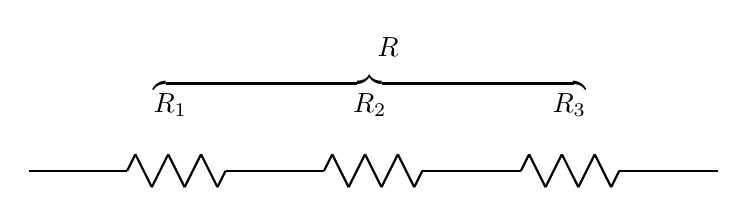
\begin{tikzpicture}[scale=2.5][line cap=round,line join=round,>=triangle 45,x=1cm,y=1cm]
			\draw (-0.4152701058878135,2.5331448905031593) node[anchor=north west] {$\overbrace{R_1\qquad\qquad\qquad R_2\qquad \qquad\qquad R_3}$};
			\draw (0.7212771477096162,2.723894079918112) node[anchor=north west] {$R$};
			\draw [line width=0.8pt] (0,2)-- (-0.04166666666666666,1.9166666666666667);
			\draw [line width=0.8pt] (-0.04166666666666666,1.9166666666666667)-- (-0.125,2.0833333333333335);
			\draw [line width=0.8pt] (-0.125,2.0833333333333335)-- (-0.20833333333333334,1.9166666666666667);
			\draw [line width=0.8pt] (-0.20833333333333334,1.9166666666666667)-- (-0.2916666666666667,2.0833333333333335);
			\draw [line width=0.8pt] (-0.2916666666666667,2.0833333333333335)-- (-0.375,1.9166666666666667);
			\draw [line width=0.8pt] (-0.375,1.9166666666666667)-- (-0.45833333333333337,2.0833333333333335);
			\draw [line width=0.8pt] (-0.45833333333333337,2.0833333333333335)-- (-0.5,2);
			\draw [line width=0.8pt] (0,2)-- (0,2);
			\draw [line width=0.8pt] (-0.5,2)-- (-0.5,2);
			\draw [line width=0.8pt] (0.5,2)-- (0.5416666666666666,2.0833333333333335);
			\draw [line width=0.8pt] (0.5416666666666666,2.0833333333333335)-- (0.625,1.9166666666666667);
			\draw [line width=0.8pt] (0.625,1.9166666666666667)-- (0.7083333333333334,2.0833333333333335);
			\draw [line width=0.8pt] (0.7083333333333334,2.0833333333333335)-- (0.7916666666666666,1.9166666666666667);
			\draw [line width=0.8pt] (0.7916666666666666,1.9166666666666667)-- (0.875,2.0833333333333335);
			\draw [line width=0.8pt] (0.875,2.0833333333333335)-- (0.9583333333333334,1.9166666666666667);
			\draw [line width=0.8pt] (0.9583333333333334,1.9166666666666667)-- (1,2);
			\draw [line width=0.8pt] (0.5,2)-- (0.5,2);
			\draw [line width=0.8pt] (1,2)-- (1,2);
			\draw [line width=0.8pt] (1.5,2)-- (1.5416666666666667,2.0833333333333335);
			\draw [line width=0.8pt] (1.5416666666666667,2.0833333333333335)-- (1.625,1.9166666666666667);
			\draw [line width=0.8pt] (1.625,1.9166666666666667)-- (1.7083333333333333,2.0833333333333335);
			\draw [line width=0.8pt] (1.7083333333333333,2.0833333333333335)-- (1.7916666666666667,1.9166666666666667);
			\draw [line width=0.8pt] (1.7916666666666667,1.9166666666666667)-- (1.875,2.0833333333333335);		\draw [line width=0.8pt] (1.875,2.0833333333333335)-- (1.9583333333333333,1.9166666666666667);
			\draw [line width=0.8pt] (1.9583333333333333,1.9166666666666667)-- (2,2);
			\draw [line width=0.8pt] (1.5,2)-- (1.5,2);
			\draw [line width=0.8pt] (2,2)-- (2,2);	
			\draw [line width=0.8pt] (0,2)-- (0.5,2);
			\draw [line width=0.8pt] (1,2)-- (1.5,2);
			\draw [line width=0.8pt] (2,2)-- (2.5,2);
			\draw [line width=0.8pt] (-0.5,2)-- (-1,2);
		\end{tikzpicture}
	\end{figure}
	\begin{align*}
		R &= R_1 + R_2 + R_3 + \cdots\\
		L &= L_1 + L_2 + L_3 + \cdots\\
		\dfrac{1}{C} &= \dfrac{1}{C_1} + \dfrac{1}{C_2} + \dfrac{1}{C_3}+ \cdots\\
		Z &= Z_1 + Z_2+ Z_3 + \cdots
	\end{align*}
	\item In parallel: 
	\begin{figure}[h!]
		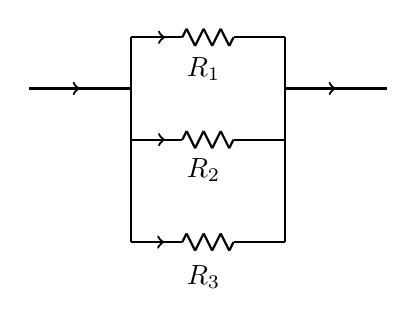
\begin{tikzpicture}[scale=1.3][line cap=round,line join=round,>=triangle 45,x=1cm,y=1cm]
			\draw (-2.55,0.9) node[anchor=north west] {$R_1$};
			\draw [line width=0.8pt] (-3,0.5)-- (-4,0.5);
			\draw [line width=0.8pt] (-1.5,0.5)-- (-0.5,0.5);
			\draw [line width=0.8pt] (-3,1)-- (-3,-1);
			\draw [line width=0.8pt] (-1.5,-1)-- (-1.5,1);
			\draw [line width=0.8pt] (-2.5,1)-- (-2.4583333333333335,1.0833333333333333);
			\draw [line width=0.8pt] (-2.4583333333333335,1.0833333333333333)-- (-2.375,0.9166666666666666);
			\draw [line width=0.8pt] (-2.375,0.9166666666666666)-- (-2.2916666666666665,1.0833333333333333);
			\draw [line width=0.8pt] (-2.2916666666666665,1.0833333333333333)-- (-2.2083333333333335,0.9166666666666666);
			\draw [line width=0.8pt] (-2.2083333333333335,0.9166666666666666)-- (-2.125,1.0833333333333333);
			\draw [line width=0.8pt] (-2.125,1.0833333333333333)-- (-2.0416666666666665,0.9166666666666666);
			\draw [line width=0.8pt] (-2.0416666666666665,0.9166666666666666)-- (-2,1);
			\draw [line width=0.8pt] (-3,1)-- (-2.5,1);
			\draw [line width=0.8pt] (-2,1)-- (-1.5,1);
			\draw [line width=0.8pt] (-2.5,0)-- (-2.4583333333333335,0.08333333333333333);
			\draw [line width=0.8pt] (-2.4583333333333335,0.08333333333333333)-- (-2.375,-0.08333333333333333);
			\draw [line width=0.8pt] (-2.375,-0.08333333333333333)-- (-2.2916666666666665,0.08333333333333333);
			\draw [line width=0.8pt] (-2.2916666666666665,0.08333333333333333)-- (-2.2083333333333335,-0.08333333333333333);
			\draw [line width=0.8pt] (-2.2083333333333335,-0.08333333333333333)-- (-2.125,0.08333333333333333);
			\draw [line width=0.8pt] (-2.125,0.08333333333333333)-- (-2.0416666666666665,-0.08333333333333333);
			\draw [line width=0.8pt] (-2.0416666666666665,-0.08333333333333333)-- (-2,0);
			\draw [line width=0.8pt] (-3,0)-- (-2.5,0);
			\draw [line width=0.8pt] (-2,0)-- (-1.5,0);
			\draw [line width=0.8pt] (-2.5,-1)-- (-2.4583333333333335,-0.9166666666666666);
			\draw [line width=0.8pt] (-2.4583333333333335,-0.9166666666666666)-- (-2.375,-1.0833333333333333);
			\draw [line width=0.8pt] (-2.375,-1.0833333333333333)-- (-2.2916666666666665,-0.9166666666666666);
			\draw [line width=0.8pt] (-2.2916666666666665,-0.9166666666666666)-- (-2.2083333333333335,-1.0833333333333333);
			\draw [line width=0.8pt] (-2.2083333333333335,-1.0833333333333333)-- (-2.125,-0.9166666666666666);
			\draw [line width=0.8pt] (-2.125,-0.9166666666666666)-- (-2.0416666666666665,-1.0833333333333333);
			\draw [line width=0.8pt] (-2.0416666666666665,-1.0833333333333333)-- (-2,-1);
			\draw [line width=0.8pt] (-3,-1)-- (-2.5,-1);
			\draw [line width=0.8pt] (-2,-1)-- (-1.5,-1);
			\draw [->,line width=0.8pt] (-4,0.5) -- (-3.5,0.5);
			\draw [->,line width=0.8pt] (-1.5,0.5) -- (-1,0.5);
			\draw (-2.55,-0.09) node[anchor=north west] {$R_2$};
			\draw (-2.55,-1.13) node[anchor=north west] {$R_3$};
			\draw [->,line width=0.8pt] (-3,1) -- (-2.666666666666666,1);
			\draw [->,line width=0.8pt] (-3,0) -- (-2.666666666666666,0);
			\draw [->,line width=0.8pt] (-3,-1) -- (-2.675555555555555,-1);
		\end{tikzpicture}
	\end{figure}
	\begin{align*}
		\dfrac{1}{R} &= \dfrac{1}{R_1} + \dfrac{1}{R_2} +\dfrac{1}{R_3} + \cdots\\
		\dfrac{1}{L} &= \dfrac{1}{L_1} + \dfrac{1}{L_2} +\dfrac{1}{L_3} + \cdots\\
		C &= C_1 + C_2 + C_3 + \cdots\\
		\dfrac{1}{Z} &= \dfrac{1}{Z_1} + \dfrac{1}{Z_2} +\dfrac{1}{Z_3} + \cdots
	\end{align*}
\end{itemize}
\begin{example}
	Suppose a current $I(t) = I_0 \cos t$, passes through this: 

	\begin{figure}[H]
		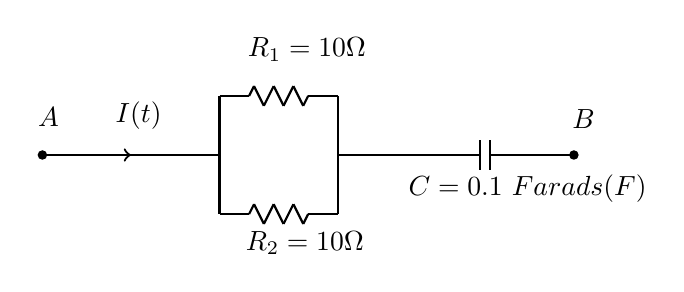
\begin{tikzpicture}[scale=1.5][line cap=round,line join=round,>=triangle 45,x=1cm,y=1cm]
			\draw (-1.36,-0.062222222222223025) node[anchor=north west] {$R_2=10\Omega$};
			\draw (-1.3422222222222224,1.573333333333327) node[anchor=north west] {$R_1=10\Omega$};
			\draw [line width=0.8pt] (-1.25,0)-- (-1.2083333333333333,0.08333333333333333);
			\draw [line width=0.8pt] (-1.2083333333333333,0.08333333333333333)-- (-1.125,-0.08333333333333333);
			\draw [line width=0.8pt] (-1.125,-0.08333333333333333)-- (-1.0416666666666667,0.08333333333333333);
			\draw [line width=0.8pt] (-1.0416666666666667,0.08333333333333333)-- (-0.9583333333333334,-0.08333333333333333);
			\draw [line width=0.8pt] (-0.9583333333333334,-0.08333333333333333)-- (-0.875,0.08333333333333333);
			\draw [line width=0.8pt] (-0.875,0.08333333333333333)-- (-0.7916666666666666,-0.08333333333333333);
			\draw [line width=0.8pt] (-0.7916666666666666,-0.08333333333333333)-- (-0.75,0);
			\draw [line width=0.8pt] (-1.5,0)-- (-1.25,0);
			\draw [line width=0.8pt] (-0.75,0)-- (-0.5,0);
			\draw [line width=0.8pt] (-1.25,1)-- (-1.2083333333333333,1.0833333333333333);
			\draw [line width=0.8pt] (-1.2083333333333333,1.0833333333333333)-- (-1.125,0.9166666666666666);
			\draw [line width=0.8pt] (-1.125,0.9166666666666666)-- (-1.0416666666666667,1.0833333333333333);
			\draw [line width=0.8pt] (-1.0416666666666667,1.0833333333333333)-- (-0.9583333333333334,0.9166666666666666);
			\draw [line width=0.8pt] (-0.9583333333333334,0.9166666666666666)-- (-0.875,1.0833333333333333);
			\draw [line width=0.8pt] (-0.875,1.0833333333333333)-- (-0.7916666666666666,0.9166666666666666);
			\draw [line width=0.8pt] (-0.7916666666666666,0.9166666666666666)-- (-0.75,1);
			\draw [line width=0.8pt] (-1.5,1)-- (-1.25,1);
			\draw [line width=0.8pt] (-0.75,1)-- (-0.5,1);
			\draw [line width=0.8pt] (-1.5,1)-- (-1.5,0);
			\draw [line width=0.8pt] (-0.5,1)-- (-0.5,0);
			\draw [line width=0.8pt] (-0.5,0.5)-- (0.5,0.5);
			\draw [line width=0.8pt] (-1.5,0.5)-- (-3,0.5);
			\draw [->,line width=0.8pt] (-3,0.5) -- (-2.25,0.5);
			\draw [line width=0.8pt] (0.5,0.5)-- (0.7083333333333334,0.5);
			\draw [line width=0.8pt] (1,0.5)-- (0.7916666666666666,0.5);
			\draw [line width=0.8pt] (0.7083333333333334,0.625)-- (0.7083333333333334,0.375);
			\draw [line width=0.8pt] (0.7916666666666666,0.625)-- (0.7916666666666666,0.375);
			\draw [line width=0.8pt] (1,0.5)-- (1.5,0.5);
			\draw (-2.4622222222222225,1.0311111111111066) node[anchor=north west] {$I(t)$};
			\draw (-3.12,0.9866666666666624) node[anchor=north west] {$A$};
			\draw (1.4044444444444446,0.9688888888888847) node[anchor=north west] {$B$};
			\draw (0.01777777777777778,0.41777777777777536) node[anchor=north west] {$C=0.1 \ Farads(F)$};
			\begin{scriptsize}
				\draw [fill=black] (-3,0.5) circle (1pt);
				\draw [fill=black] (1.5,0.5) circle (1pt);
			\end{scriptsize}
		\end{tikzpicture}
	\end{figure}
	
	Find $V(t)$, the difference in electrical potential energy between $A$ and $B$
	
	\underline{\textbf{Solution}}: 
	
	\begin{figure}[H]
		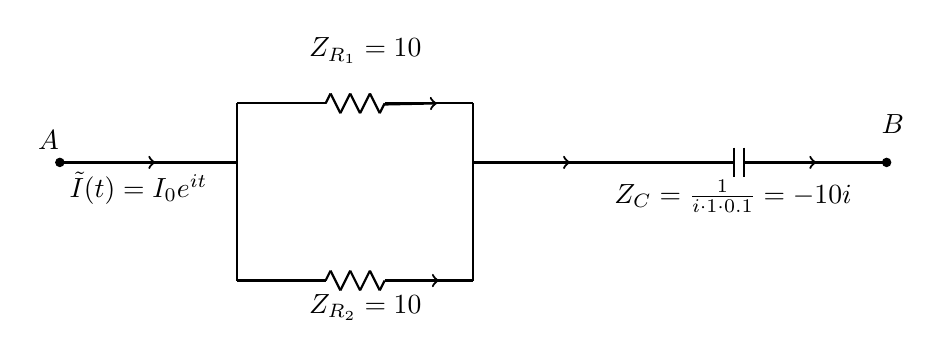
\begin{tikzpicture}[scale=1.5][line cap=round,line join=round,>=triangle 45,x=1cm,y=1cm]
			\draw (-2.4727988094140407,1.6361413165955456) node[anchor=north west] {$Z_{R_1}=10$};
			\draw [line width=0.8pt] (-2.25,-0.5)-- (-2.2083333333333335,-0.4166666666666667);
			\draw [line width=0.8pt] (-2.2083333333333335,-0.4166666666666667)-- (-2.125,-0.5833333333333334);
			\draw [line width=0.8pt] (-2.125,-0.5833333333333334)-- (-2.0416666666666665,-0.4166666666666667);
			\draw [line width=0.8pt] (-2.0416666666666665,-0.4166666666666667)-- (-1.9583333333333333,-0.5833333333333334);
			\draw [line width=0.8pt] (-1.9583333333333333,-0.5833333333333334)-- (-1.875,-0.4166666666666667);
			\draw [line width=0.8pt] (-1.875,-0.4166666666666667)-- (-1.7916666666666667,-0.5833333333333334);
			\draw [line width=0.8pt] (-1.7916666666666667,-0.5833333333333334)-- (-1.75,-0.5);
			\draw [line width=0.8pt] (-3,-0.5)-- (-2.25,-0.5);
			\draw [line width=0.8pt] (-1.75,-0.5)-- (-1,-0.5);
			\draw [line width=0.8pt] (-2.25,1)-- (-2.2083333333333335,1.0833333333333333);
			\draw [line width=0.8pt] (-2.2083333333333335,1.0833333333333333)-- (-2.125,0.9166666666666666);
			\draw [line width=0.8pt] (-2.125,0.9166666666666666)-- (-2.0416666666666665,1.0833333333333333);
			\draw [line width=0.8pt] (-2.0416666666666665,1.0833333333333333)-- (-1.9583333333333333,0.9166666666666666);
			\draw [line width=0.8pt] (-1.9583333333333333,0.9166666666666666)-- (-1.875,1.0833333333333333);
			\draw [line width=0.8pt] (-1.875,1.0833333333333333)-- (-1.7916666666666667,0.9166666666666666);
			\draw [line width=0.8pt] (-1.7916666666666667,0.9166666666666666)-- (-1.75,1);
			\draw [line width=0.8pt] (-3,1)-- (-2.25,1);
			\draw [line width=0.8pt] (-1.75,1)-- (-1,1);
			\draw [line width=0.8pt] (1,0.5)-- (1.2083333333333333,0.5);
			\draw [line width=0.8pt] (1.5,0.5)-- (1.2916666666666667,0.5);
			\draw [line width=0.8pt] (1.2083333333333333,0.625)-- (1.2083333333333333,0.375);
			\draw [line width=0.8pt] (1.2916666666666667,0.625)-- (1.2916666666666667,0.375);
			\draw [line width=0.8pt] (1.5,0.5)-- (2.5,0.5);
			\draw (-4.5,0.5) node[anchor=north west] {$\tilde{I}(t)=I_0e^{it}$};
			\draw (-4.7678511966796515,0.8504477065406559) node[anchor=north west] {$A$};
			\draw (2.375757810529975,0.9848426661553081) node[anchor=north west] {$B$};
			\draw (0.11171964471389924,0.43692475388018776) node[anchor=north west] {$Z_C=\frac{1}{i\cdot1\cdot0.1}=-10i$};
			\draw [line width=0.8pt] (-1,1)-- (-1,0.5);
			\draw [line width=0.8pt] (-1,0.5)-- (-1,-0.5);
			\draw [line width=0.8pt] (-3,1)-- (-3,0.5);
			\draw [line width=0.8pt] (-3,0.5)-- (-3,-0.5);
			\draw [line width=0.8pt] (-4.5,0.5)-- (-3,0.5);
			\draw [line width=0.8pt] (-1,0.5)-- (1,0.5);
			\draw [->,line width=0.8pt] (-4.5,0.5) -- (-3.6898720450852003,0.5);
			\draw [->,line width=0.8pt] (-1.7547447843933128,0.9905104312133761) -- (-1.306134363426703,1);
			\draw [->,line width=0.8pt] (-1.7418713589986865,-0.5) -- (-1.2890466381101549,-0.5);
			\draw [->,line width=0.8pt] (-1,0.5) -- (-0.178344492534511,0.5);
			\draw [->,line width=0.8pt] (1.5,0.5) -- (1.9063579960843895,0.5);
			\draw (-2.4727988094140407,-0.5348541848719125) node[anchor=north west] {$Z_{R_2}=10$};
			\begin{scriptsize}
				\draw [fill=black] (-4.5,0.5) circle (1pt);
				\draw [fill=black] (2.5,0.5) circle (1pt);
			\end{scriptsize}
		\end{tikzpicture}
	\end{figure}

	Let's use the complex version of ``Ohm's Law''. We have $\dfrac{1}{Z_R} = \dfrac{1}{Z_{R_1}} + \dfrac{1}{Z_{R_2}} = \dfrac{1}{10} + \dfrac{1}{10} = \dfrac{1}{5}$, so $Z_R = 5$. 

	Combine the resistor and capacitor in series: $Z = Z_R + Z_C = 5-10i$. 

	So, the complex voltage is \begin{align*}
		\widetilde{V} &= Z \widetilde{I}\\
		&= (5-10i)I_0e^{it}\\
		&=5I_0(1-2i)e^{it}\\
		&=5I_0\sqrt{5}e^{i\arctan -2} e^{it}
	\end{align*}
	So, $V(t) = Re(\widetilde{V}(t)) \approx 5\sqrt{5} I_0 \cos(t-1.107)$
	\begin{figure}[H]
		\begin{tikzpicture}[scale=1.5][line cap=round,line join=round,>=triangle 45,x=1cm,y=1cm]
			\begin{axis}[
				x=1cm,y=1cm,
				axis lines=middle,
				xmin=-1.9140740740740745,
				xmax=3.3718518518518503,
				ymin=-2.1896296296296267,
				ymax=0.583703703703702,
				xtick={0,1},
				ytick={-2,-1,...,0},]
				\draw [->,line width=0.8pt] (0,0) -- (1,-2);	
				\draw (0.38,-0.4) node[anchor=north west] {$\arctan2$};
				\end{axis}
			\draw [shift={(1.5,1.75)},<-,line width=1pt] (-2:0.65) arc (-63.43494882292201:0:0.5333333333333332);
		\end{tikzpicture}
	\end{figure}
\end{example}

\subsection{Sets in the Complex Plane}
\begin{definition}
	\textbf{\underline{Neighborhood of $z_0$}} is $$N_\epsilon(z_0) = \{z \in \mathbb{C} : |z-z_0| < \epsilon\}$$ where $\epsilon > 0$ is real
\end{definition}
\begin{definition}
	\textbf{\underline{Deleted Neighborhood of $z_0$}} is $$DN_\epsilon(z_0) = \{z \in \mathbb{C} : 0 < |z-z_0| < \epsilon\}$$ where $\epsilon > 0$ is real
\end{definition}
\begin{example}
	For $z_0 = 1+i$, consider $|z-(1+i)| < 1$. The neighborhood of $z_0$ and deleted neighborhood of $z_0$ is as follows: 

	\begin{figure}[H]
		\definecolor{uu}{rgb}{0.3,0.3,0.3}
		\begin{tikzpicture}[line cap=round,line join=round,>=triangle 45,x=1cm,y=1cm]
			\draw[->] (-1,0)--(5,0);
			\draw[->] (0,-1)--(0,5);
			\draw [dashed,line width=1.2pt,fill=black,fill opacity=0.27] (2,2) circle (2cm);
			\draw (2.05,3.2) node[anchor=north west] {$N_1(1+i)$};
			\draw [fill=black] (2,2) circle (1.5pt);
			\draw [fill=uu] (0,2) circle (1pt);
			\draw[color=uu] (-0.25,2.) node {i};
			\draw [fill=black] (0,4) circle (1pt);
			\draw[color=black] (-0.25,4) node {2i};
			\draw [fill=uu] (2,0) circle (2pt);
			\draw[color=uu] (2,-0.35) node {1};
			\draw [fill=black] (4,0) circle (1pt);
			\draw[color=black] (4,-0.35) node {2};
		\end{tikzpicture}
		\begin{tikzpicture}[line cap=round,line join=round,>=triangle 45,x=1cm,y=1cm]
			\draw[->] (-1,0)--(5,0);
			\draw[->] (0,-1)--(0,5);
			\draw [dashed,line width=1.2pt,fill=black,fill opacity=0.27] (2,2) circle (2cm);
			\draw (1.7,3.1) node[anchor=north west] {$DN_1(1+i)$};
			\draw [color=black] (2,2) circle (1.5pt);
			\draw [fill=uu] (0,2) circle (1pt);
			\draw[color=uu] (-0.25,2.) node {i};
			\draw [fill=black] (0,4) circle (1pt);
			\draw[color=black] (-0.25,4) node {2i};
			\draw [fill=uu] (2,0) circle (2pt);
			\draw[color=uu] (2,-0.35) node {1};
			\draw [fill=black] (4,0) circle (1pt);
			\draw[color=black] (4,-0.35) node {2};
		\end{tikzpicture}
	\end{figure}
\end{example}
\begin{definition}
	Let $S \subseteq \mathbb{C}$: \begin{itemize}
		\item $z_0$ is an \underline{\textbf{interior point}} of $S$ if there exists a neighborhood of $z_0$ which contains only points in $S$
		\item $z_0$ is an \underline{\textbf{exterior point}} of $S$ if there exists a neighborhood of $z_0$ which contains no points in $S$
		\item $z_0$ is a \underline{\textbf{boundary point}} of $S$ if every neighborhood of $z_0$ contains some points in $S$ and some points not. 
		\item \underline{\textbf{Boundary of $S$}} is the set of all boundary points of $S$
		\item $S$ is \underline{\textbf{open}} if it contains none of its boundary points
		\item $S$ is \underline{\textbf{closed}} if it contains all of its boundary points, equivalently if its complement is open. 
		\item Note that $S$ could be both open and closed, when it does not have any boundary points
	\end{itemize}
	\begin{figure}[H]
		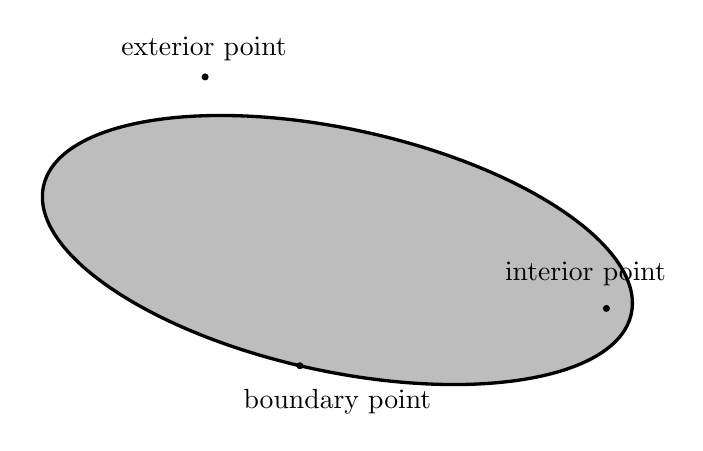
\begin{tikzpicture}[scale=0.7][line cap=round,line join=round,>=triangle 45,x=1cm,y=1cm]
			\draw [rotate around={-12.2550245737389:(0.82,-1.26)},line width=1.2pt,fill=black,fill opacity=0.26] (0.82,-1.26) ellipse (5.456218028894557cm and 2.1982527559027356cm);
			\draw [fill=black] (5.7,-2.32) circle (1.5pt);
			\draw[color=black] (5.32,-1.69) node {interior point};
			\draw [fill=black] (0.14,-3.36) circle (1.5pt);
			\draw[color=black] (0.82,-4.01) node {boundary point};
			\draw [fill=black] (-1.58,1.88) circle (1.5pt);
			\draw[color=black] (-1.6,2.39) node {exterior point};
		\end{tikzpicture}
		\end{figure}
\end{definition}
\begin{example}
	Note that \begin{itemize}
		\item $N_1(1+i)$ is open
		\item $\mathbb{C}$ is both open and closed
		\item $|z-z_0| \leq 1$ is closed
		\item The figure below: it is neither open nor closed. 
		\begin{figure}[H]
			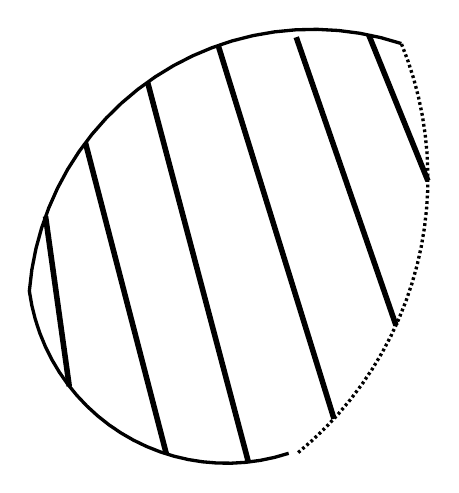
\begin{tikzpicture}[scale=1.3][line cap=round,line join=round,>=triangle 45,x=1cm,y=1cm]
				\draw [shift={(-2.2,-0.04)},line width=1.2pt,dash pattern=on 1pt off 1pt]  plot[domain=-0.8834434406912877:0.38931672183314087,variable=\t]({1*3.467333269243094*cos(\t r)+0*3.467333269243094*sin(\t r)},{0*3.467333269243094*cos(\t r)+1*3.467333269243094*sin(\t r)});
				\draw [shift={(0.14,-1.36)},line width=1.2pt]  plot[domain=1.2527427180455013:3.0628086926006493,variable=\t]({1*2.7752379743583204*cos(\t r)+0*2.7752379743583204*sin(\t r)},{0*2.7752379743583204*cos(\t r)+1*2.7752379743583204*sin(\t r)});
				\draw [shift={(-0.7,-0.88)},line width=1.2pt]  plot[domain=3.2765392412560086:5.030186986194582,variable=\t]({1*1.944306222620606*cos(\t r)+0*1.944306222620606*sin(\t r)},{0*1.944306222620606*cos(\t r)+1*1.944306222620606*sin(\t r)});
				\draw [line width=2pt] (-2.4682557768735838,-0.41187151887202067)-- (-2.2364548804155135,-2.071483565882702);
				\draw [line width=2pt] (-2.078453794925833,0.3074557187822542)-- (-1.2880175887067855,-2.733257133452524);
				\draw [line width=2pt] (-1.471600098553103,0.8993563102494704)-- (-0.4865924018176054,-2.8125588954438703);
				\draw [line width=2pt] (-0.7815545996879623,1.2577629636990497)-- (0.34969242697916547,-2.3897805275823303);
				\draw [line width=2pt] (-0.01921974959665283,1.3379878398032463)-- (0.9554416977355595,-1.4772152560391683);
				\draw [line width=2pt] (0.6895144756631459,1.3602903623247886)-- (1.2672454540513378,-0.06467714246696885);
			\end{tikzpicture}
		\end{figure}
	\end{itemize}
\end{example}
\begin{definition}
	For $S \subseteq \mathbb{C}$: \begin{itemize}
		\item \underline{\textbf{Closure}} of $S$ is $S$ plus its boundary.
		\item An open set $S$ is \underline{\textbf{connected}} if any two points in $S$ can be connected by a polygonal path lying entirely in $S$
		\item A \underline{\textbf{domain}} is an open connected set. We should not confuse this with ``domain of a function''
		\item A \underline{\textbf{region}} is a domain plus some, none, or all of its boundary points. 
		\item $S$ is \underline{\textbf{bounded}} if there exists $R \in \mathbb{R}$ such that $|z| < R$ for all $z \in S$
	\end{itemize}
	\begin{figure}[H]
		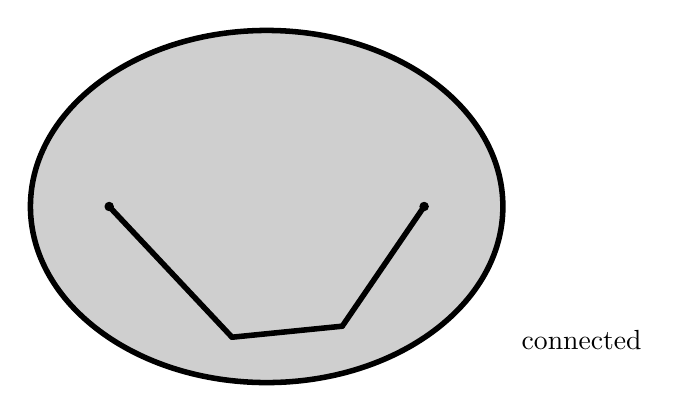
\begin{tikzpicture}[line cap=round,line join=round,>=triangle 45,x=1cm,y=1cm]
			\draw [rotate around={0:(0,0)},line width=2pt,fill=black,fill opacity=0.19] (0,0) ellipse (3cm and 2.23606797749979cm);
			\draw [line width=2pt] (-2,0)-- (-0.44,-1.66);
			\draw [line width=2pt] (-0.44,-1.66)-- (0.96,-1.52);
			\draw [line width=2pt] (0.96,-1.52)-- (2,0);
			\begin{scriptsize}
				\draw [fill=black] (-2,0) circle (1.5pt);
				\draw [fill=black] (2,0) circle (1.5pt);
			\end{scriptsize}
			\draw[color=black] (4,-1.69) node {connected};
		\end{tikzpicture}
		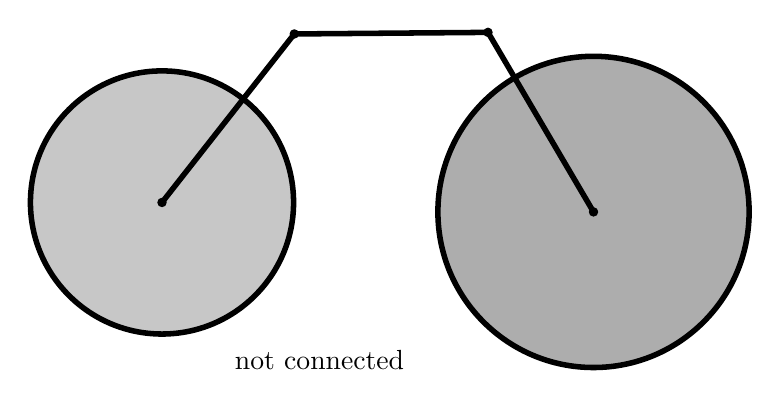
\begin{tikzpicture}[line cap=round,line join=round,>=triangle 45,x=1cm,y=1cm]
			\draw [line width=2pt,fill=black,fill opacity=0.22] (-2,0) circle (1.6709278859364338cm);
			\draw [line width=2pt,fill=black,fill opacity=0.32] (3.48,-0.12) circle (1.9762590923257002cm);
			\draw [line width=2pt] (-2,0)-- (-0.32,2.14);
			\draw [line width=2pt] (-0.32,2.14)-- (2.14,2.16);
			\draw [line width=2pt] (2.14,2.16)-- (3.48,-0.12);
			\begin{scriptsize}
				\draw [fill=black] (-2,0) circle (1.5pt);
				\draw [fill=black] (-0.32,2.14) circle (1.5pt);
				\draw [fill=black] (2.14,2.16) circle (1.5pt);
				\draw [fill=black] (3.48,-0.12) circle (1.5pt);		
			\end{scriptsize}
			\draw[color=black] (0,-2) node {not connected};
		\end{tikzpicture}
	\end{figure}
\end{definition}
\begin{theorem}
	If $u(x, y)$, defined on a domain $D$, satisfies $$\dfrac{\partial u}{\partial x} = \dfrac{\partial u}{\partial y} = 0$$ for all points in $D$, then $u(x, y) = $ constant in $D$. 
\end{theorem}
\begin{example}
	Suppose we have $S_1$ and $S_2$ like this: 
	\begin{figure}[H]
		\begin{tikzpicture}[line cap=round,line join=round,>=triangle 45,x=1cm,y=1cm]
			\draw[->] (-5,0)--(5,0);
			\draw[->] (0,-1)--(0,5);
			\draw [rotate around={-0.83:(-2.77,1.55)},line width=0.5pt,
			dash pattern=on 1pt off 1pt] (-2.77,1.55) ellipse (1.19cm and 0.97cm);
			\draw [rotate around={-4.1:(2.52,1.56)},line width=0.5,
			dash pattern=on 1pt off 1pt] (2.52,1.56) ellipse (1.35cm and 1.22cm);
			\draw[color=black] (-2.9,1.77) node {$S_1$};
			\draw[color=black] (2.56,1.89) node {$S_2$};
		\end{tikzpicture}
	\end{figure}
	
	in which we have $u(x,y) = 0$ on $S_1$ and $u(x,y) = 1$ on $S_2$. 

	Then, $\dfrac{\partial u}{\partial x} = \dfrac{\partial u}{\partial y} = 0$ on $S_1 \cup S_2$, but $u(x,y)$ is not constant on $S_1 \cup S_2$.

	Why does not the theorem hold? Well this is because $S_1 \cup S_2$ is not connected, so it's not a domain. 
\end{example}
The Extended Complex Plane: 

The ``neighborhood of $\infty$'' is defined as: $$N_\epsilon(\infty) = \{z \in \mathbb{C} : |z| > \dfrac{1}{\epsilon}\}$$ for some real $\epsilon > 0$
\newpage
The Riemann sphere: 

\begin{figure}[h!]
	\definecolor{zzttqq}{rgb}{0.6,0.2,0}
	\begin{tikzpicture}[scale=0.8][line cap=round,line join=round,>=triangle 45,x=1cm,y=1cm]
		\fill[line width=2pt,color=zzttqq,fill=zzttqq,fill opacity=0.10000000149011612] (-4,2) -- (-8,-2) -- (5,-2) -- (9,2) -- cycle;
		\draw [->,line width=2pt] (0,-4.801835999999982) -- (0,5.06);
		\draw [->,line width=2pt] (-5,0) -- (6,0);
		\draw [->,line width=2pt] (3.5,3.5) -- (-4,-4);
		\draw [shift={(0,0)},line width=1pt]  plot[domain=0:3.141592653589793,variable=\t]({1*4*cos(\t r)+0*4*sin(\t r)},{0*4*cos(\t r)+1*4*sin(\t r)});
		\draw [shift={(0,0)},line width=1pt,dash pattern=on 1pt off 1pt]  plot[domain=3.141592653589793:6.283185307179586,variable=\t]({1*4*cos(\t r)+0*4*sin(\t r)},{0*4*cos(\t r)+1*4*sin(\t r)});
		\draw [rotate around={0:(-0.01,0)},line width=1.2pt,dash pattern=on 1pt off 1pt] (-0.01,0) ellipse (3.998253390825929cm and 1.4398368578596104cm);
		\draw [line width=1pt,dash pattern=on 1pt off 1pt] (0,4)-- (5,-1);
		\draw (-10,4.68) node[anchor=north west] {Riemann Sphere $x_1^2+x_2^2+x_3^2=1$};
		\draw [->,line width=1pt] (-4.44,3.8) -- (-2.8879528204616975,2.7676214529424588);
		\draw (3.5,3) node[anchor=north west] {``Stereographic Projection''};
		\draw[color=black] (0.18,-3.65) node {$d$};
		\draw [fill=black] (0,4) circle (1pt);
		\draw[color=black] (-0.6,4.49) node {(0,0,1)};
		\draw[color=black] (-1.94,1.07) node {$e$};
		\draw [fill=black] (5,-1) circle (1pt);
		\draw[color=black] (5.14,-1.31) node {$(x_1, x_2)$};
		\draw [fill=black] (2.78,1.22) circle (1pt);
	\end{tikzpicture}
\end{figure}

We can define a one-to-one mapping between $x_1x_2$-plane and the sphere: 

\begin{figure}[h!]
	\definecolor{uuuuuu}{rgb}{0.27,0.27,0.27}
	\begin{tikzpicture}[scale=0.8][line cap=round,line join=round,>=triangle 45,x=1cm,y=1cm]
		\draw [line width=2pt] (0,0) circle (3cm);
		\draw [line width=2pt,domain=-7.26:10.58] plot(\x,{(-0-0*\x)/3});
		\draw (-4.26,3.08) node[anchor=north west] {2D View};
		\draw [line width=1pt,dash pattern=on 1pt off 2pt] (0,3) -- (0,-5);
		\draw [line width=1pt,dash pattern=on 1pt off 2pt,domain=0:8] plot(\x,{(--9-3*\x)/3});
		\draw [line width=1.2pt,dash pattern=on 1pt off 2pt,domain=0:8] plot(\x,{(--4.3-0.36*\x)/1.4});
		\draw [line width=1.2pt,dash pattern=on 1pt off 2pt,domain=0:8] plot(\x,{(--12-0*\x)/4});
		\draw (0.12,-3.14) node[anchor=north west] {Origin maps to South Pole};
		\draw (4.08,-0.06) node[anchor=north west] {points on circle $x_1^2+x_2^2=1$};
		\draw (0.2,4) node[anchor=north west] {``point at infinity'', corresponds to North Pole};
		\draw [fill=black] (3,0) circle (2pt);
		\draw [fill=uuuuuu] (0,3) circle (2pt);
		\draw [fill=uuuuuu] (0,-3) circle (2pt);
		\draw [fill=black] (1.4211057346355416,2.642055731998471) circle (2.5pt);
	\end{tikzpicture}
\end{figure}

See the course text for more detail, in particular: \begin{itemize}
	\item Circles and lines all map circles on the sphere
	\item Lines are just circles which pass through the ``point at infinity''
\end{itemize}
\section{Analytic Functions}
\subsection{Functions}
For a function on complex numbers: \begin{align*}
	\omega &= f(z)\\
	&=f(x+iy) \\
	&=u(x,y) + iv(x,y)
\end{align*}
We can think of it as a mapping. 
\begin{example}
	\begin{enumerate}
		\item $f(z) = z^2$. Find the images of \begin{enumerate}
			\item the first quadrant. 
			
			$f(z) = (x+iy)^2 = \underbrace{(x^2-y^2)}_{u} + i\underbrace{2xy}_{v}$ 

			\begin{figure}[H]
				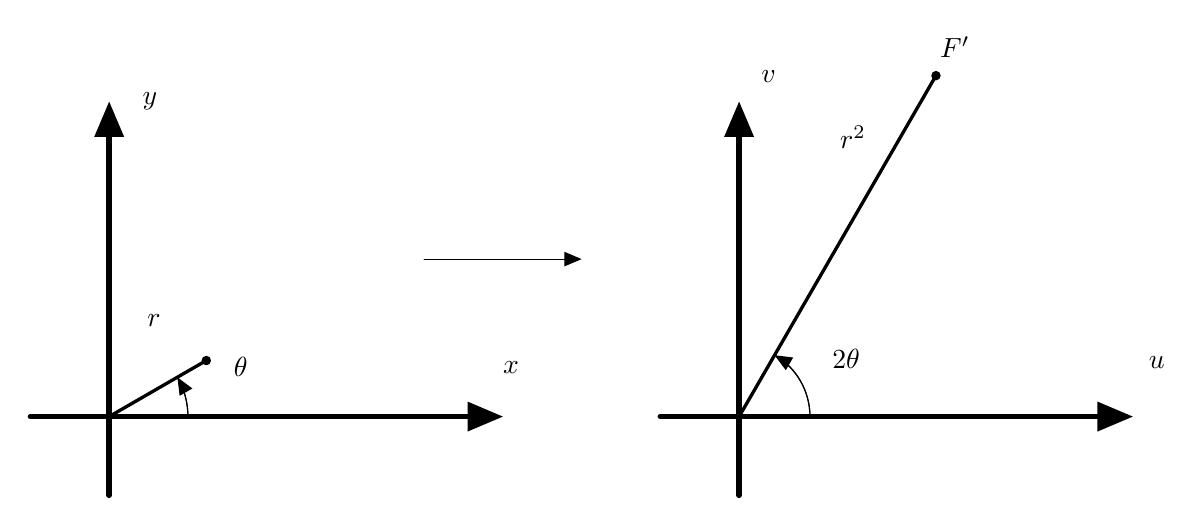
\begin{tikzpicture}[line cap=round,line join=round,>=triangle 45,x=1cm,y=1cm]
					\draw [shift={(-5,1)},line width=0.4pt] (0,0) -- (0:1) arc (0:30:1) -- cycle;
					\draw [shift={(3,1)},line width=0.4pt] (0,0) -- (0:0.9) arc (0:60:0.9) -- cycle;
					\draw [->,line width=2pt] (-6,1) -- (0,1);
					\draw [->,line width=2pt] (-5,0) -- (-5,5);
					\draw [->,line width=2pt] (2,1) -- (8,1);
					\draw [->,line width=2pt] (3,0) -- (3,5);
					\draw [shift={(-5,1)},->,line width=0.4pt] (0:1) arc (0:30:1);
					\draw [shift={(3,1)},->,line width=0.4pt] (0:0.9) arc (0:60:0.9);
					\draw [->,line width=0.4pt] (-1,3) -- (1,3);
					\draw [line width=1.2pt] (3,1)-- (5.5,5.330127018922193);
					\draw [line width=1.2pt] (-5,1)-- (-3.766891108675446,1.711935750346352);
					\draw (-4.64,2.42) node[anchor=north west] {$r$};
					\draw (4.16,4.82) node[anchor=north west] {$r^2$};
					\draw (-3.54,1.88) node[anchor=north west] {$\theta$};
					\draw (4.06,1.98) node[anchor=north west] {$2\theta$};
					\draw (-0.12,1.82) node[anchor=north west] {$x$};
					\draw (-4.7,5.24) node[anchor=north west] {$y$};
					\draw (8.08,1.88) node[anchor=north west] {$u$};
					\draw (3.16,5.52) node[anchor=north west] {$v$};
					\draw [fill=black] (5.5,5.330127018922193) circle (1.5pt);
					\draw[color=black] (5.74,5.69) node {$F'$};
					\draw [fill=black] (-3.766891108675446,1.711935750346352) circle (1.5pt);
				\end{tikzpicture}
			\end{figure}
			
			Note that $f(z) = (re^{i\theta})^2 = r^2e^{i2\theta}$ (angle is doubled)
			\item the strip $1 \leq Re(z) \leq 2$
			
			With $1 \leq x \leq 2$, the boundaries become: \begin{itemize}
				\item $x = 1 \Rightarrow \begin{dcases}
					u = 1-y^2\\
					v=2y
				\end{dcases} \Rightarrow u = 1 - \big(\dfrac{v}{2}\big)^2$, which is a parabola
				\item $x = 2 \Rightarrow \begin{dcases}
					u = 4-y^2\\
					v=4y
				\end{dcases} \Rightarrow u = 4 - \big(\dfrac{v}{4}\big)^2$, which is a parabola
			\end{itemize}
			\begin{figure}[H]
				\definecolor{qqqqff}{rgb}{0,0,1}
				\begin{tikzpicture}[line cap=round,line join=round,>=triangle 45,x=1cm,y=1cm]
					\begin{axis}[
						x=1cm,y=1cm,
						axis lines=middle,
						xmin=-1,
						xmax=4,
						ymin=-1,
						ymax=2,
						xlabel={x} ,
						ylabel={y},
						xtick=\empty,
						ytick=\empty]
					\end{axis}
					\draw[line width=0pt,fill=qqqqff,fill opacity=0.25]
					(2,3)--(2,1)--(3,1)--(3,3);
					\draw[line width=0pt,fill=qqqqff,fill opacity=0.25]
					(2,-1)--(2,1)--(3,1)--(3,-1);
					\draw (3,2) node[anchor=north west] {$x=2$};
					\draw (1,2) node[anchor=north west] {$x=1$};
					\draw [fill=black] (2,1) circle (2pt);
					\draw[color=black] (1.8,0.5) node {1};
					\draw [fill=black] (3,1) circle (2pt);
					\draw[color=black] (3.3,0.5) node {2};
					\draw [fill=black] (2.5,1) circle (2pt);
				\end{tikzpicture}
				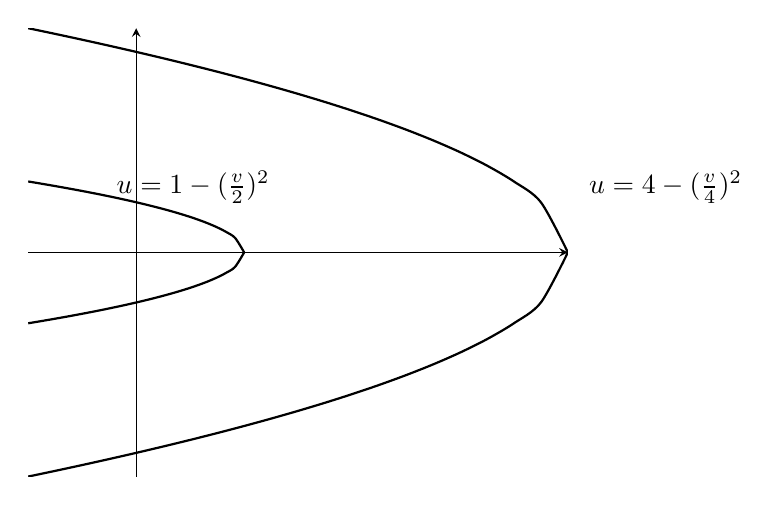
\begin{tikzpicture} 
					\begin{axis}[
						axis x line=middle,
						axis y line=middle,
						xtick=\empty,
						ytick=\empty
						]
						\addplot[smooth,thick,domain=-1:1]{2*sqrt(1-x)}; 
						\addplot[smooth,thick,domain=-1:1]{-2*sqrt(1-x)};
						\addplot[smooth,thick,domain=-1:5]{4*sqrt(4-x)}; 
						\addplot[smooth,thick,domain=-1:5]{-4*sqrt(4-x)};
					\end{axis}
				\draw (1,4) node[anchor=north west] {$u=1-(\frac{v}{2})^2$};
				\draw (7,4) node[anchor=north west] {$u=4-(\frac{v}{4})^2$};
				\end{tikzpicture}
			\end{figure}
		\end{enumerate}
		\item $f(z) = |z|$. This one maps complex plane to non-negative real axis. 
		\begin{figure}[H]
			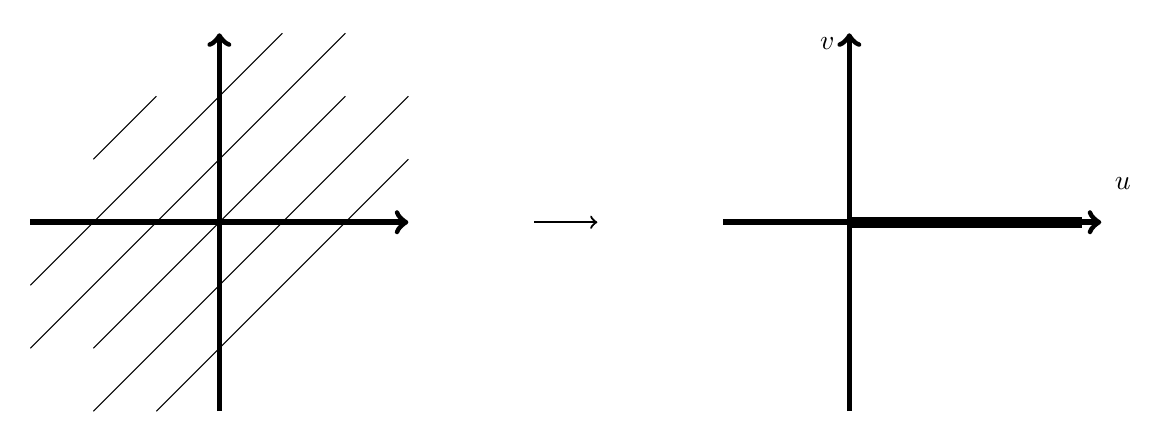
\begin{tikzpicture}[scale=0.8][line cap=round,line join=round,>=triangle 45,x=1cm,y=1cm]
				\draw [->,line width=2pt] (-3,-2) -- (-3,4);
				\draw [->,line width=2pt] (-6,1) -- (0,1);
				\draw [line width=0.4pt] (-4,3)-- (-5,2);
				\draw [line width=0.4pt] (-2,4)-- (-6,0);
				\draw [line width=0.4pt] (-1,4)-- (-6,-1);
				\draw [line width=0.4pt] (0,3)-- (-5,-2);
				\draw [line width=0.4pt] (-4,-2)-- (0,2);
				\draw [->,line width=0.8pt] (2,1) -- (3,1);
				\draw [line width=0.4pt] (-5,-1)-- (-1,3);
				\draw [->,line width=2pt] (5,1) -- (11,1);
				\draw [->,line width=2pt] (7,-2) -- (7,4);
				\draw [line width=4pt] (7,1)-- (10.7,1);
				\draw (11.06,1.86) node[anchor=north west] {$u$};
				\draw (6.38,4.08) node[anchor=north west] {$v$};
			\end{tikzpicture}
		\end{figure}
		\item $f(z) = z-z_0 = (x+iy) - (x_0+iy_0) = (x-x_0) + i(y-y_0)$. This is a translation. 
		\item $f(z) = z_0z$, so $$f(z) = r_0e^{i\theta_0}re^{i\theta} = \underbrace{r_0}_{\text{magnification}}re^{i\underbrace{\theta_0}_{\text{rotation}}+\theta} = r_0re^{i\theta_0+\theta}$$
		\item $f(z) = \overline{z} = x-iy \rightarrow \begin{dcases}
			u = x\\
			v = -y
		\end{dcases}$. This is a reflection on $y$-axis. 
		\item Find image of half-plane $Re(z) \geq 1$ under the map $\omega = f(z) = iz-3i$. 
		
		We can do this step by step. First it's a rotation of $\dfrac{\pi}{2}$ (comes from the first $i$), then its a shift down 3 units. 

		\begin{figure}[H]
			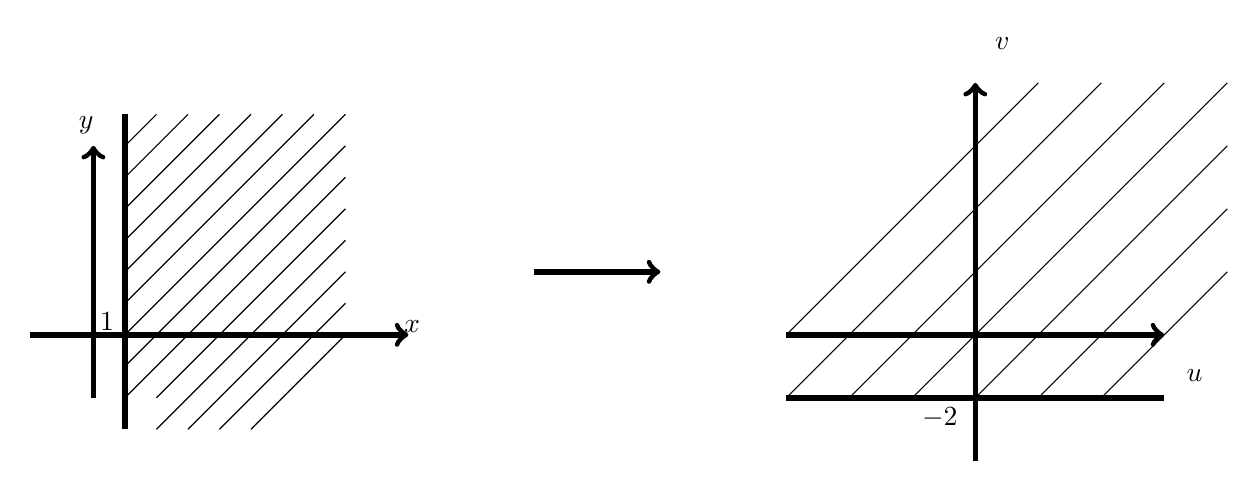
\begin{tikzpicture}[scale=0.4][line cap=round,line join=round,>=triangle 45,x=1cm,y=1cm]
				\draw [line width=2pt] (1,7)-- (1,-2);
				\draw [line width=0.4pt] (1,6)-- (2,7);
				\draw [line width=0.4pt] (1,5)-- (3,7);
				\draw [line width=0.4pt] (1,4)-- (4,7);
				\draw [line width=0.4pt] (1,3)-- (5,7);
				\draw [line width=0.4pt] (1,2)-- (6,7);
				\draw [line width=0.4pt] (1,1)-- (7,7);
				\draw [line width=0.4pt] (1,0)-- (8,7);
				\draw [line width=0.4pt] (1,-1)-- (8,6);
				\draw [line width=0.4pt] (1,-2)-- (8,5);
				\draw [line width=2pt] (1,-2)-- (1,-3);
				\draw [line width=0.4pt] (2,-2)-- (8,4);
				\draw [line width=0.4pt] (2,-3)-- (8,3);
				\draw [line width=0.4pt] (3,-3)-- (8,2);
				\draw [line width=0.4pt] (4,-3)-- (8,1);
				\draw [line width=0.4pt] (5,-3)-- (8,0);
				\draw [->,line width=2pt] (0,-2) -- (0,6);
				\draw [->,line width=2pt] (-2,0) -- (10,0);
				\draw (-0.0975,1) node[anchor=north west] {$1$};
				\draw (-0.7725,7.2375) node[anchor=north west] {$y$};
				\draw (9.555,0.7575) node[anchor=north west] {$x$};
				\draw [->,line width=2pt] (14,2) -- (18,2);
				\draw [->,line width=2pt] (22,0) -- (34,0);
				\draw [line width=2pt] (22,-2)-- (34,-2);
				\draw [->,line width=2pt] (28,-4) -- (28,8);
				\draw [line width=0.4pt] (22,0)-- (30,8);
				\draw [line width=0.4pt] (24,-2)-- (34,8);
				\draw [line width=0.4pt] (26,-2)-- (36,8);
				\draw [line width=0.4pt] (28,-2)-- (36,6);
				\draw [line width=0.4pt] (30,-2)-- (36,4);
				\draw [line width=0.4pt] (32,-2)-- (36,2);
				\draw [line width=0.4pt] (22,-2)-- (32,8);
				\draw (34.395,-0.795) node[anchor=north west] {$u$};
				\draw (28.32,9.735) node[anchor=north west] {$v$};
				\draw (26,-2) node[anchor=north west] {$-2$};
				\begin{scriptsize}
					\draw [fill=black] (28,-2) circle (1.5pt);
				\end{scriptsize}
			\end{tikzpicture}
		\end{figure}

		The image is the half-plane $v\geq -2$. 
		\item Inversion mapping. $f(z) = \dfrac{1}{z} = \dfrac{1}{re^{i\theta}} = \dfrac{1}{r}e^{-i\theta}$. So, it's a scaling by $r$, and then reflection through the $x$-axis. 
		
		For this mapping, unit circle maps to the unit circle. Outside points go to inside, and inside points go to outside. 

		\begin{figure}[H]
			\definecolor{uuu}{rgb}{0.3,0.3,0.3}
			\begin{tikzpicture}[scale=1.5][line cap=round,line join=round,>=triangle 45,x=1cm,y=1cm]
				\draw [shift={(0,0)},line width=2pt] (0,0) -- (0:0.4193384935264618) arc (0:45:0.4193384935264618) -- cycle;
				\draw [->,line width=1.2pt] (-3,0) -- (3,0);
				\draw [->,line width=1.2pt] (0,-3) -- (0,3);
				\draw [line width=2pt] (0,0) circle (2cm);
				\draw [line width=0.4pt,dash pattern=on 1pt off 1pt] (-2,2)-- (2,-2);
				\draw [line width=0.4pt,dash pattern=on 1pt off 1pt] (-2,-2)-- (2,2);
				\draw [->,line width=1.2pt] (-2,2) -- (-1,-1);
				\draw [->,line width=1.2pt] (1,1) -- (2,-2);
				\draw [->,line width=1.2pt] (1.414213562373095,1.414213562373095) -- (1.414213562373095,-1.414213562373095);
				\begin{scriptsize}
					\draw [fill=uuu] (1.414213562373095,1.414213562373095) circle (1.5pt);
					\draw [fill=uuu] (1.414213562373095,-1.414213562373095) circle (1.5pt);
					\draw [fill=black] (2,-2) circle (1.5pt);
					\draw [fill=black] (1,1) circle (1.5pt);
					\draw [fill=black] (-1,-1) circle (1.5pt);
					\draw [fill=black] (-2,2) circle (1.5pt);
				\end{scriptsize}
			\end{tikzpicture}
		\end{figure}

		\item Image of circle $(x-1)^2+y^2 = 1$ under $f(z) = \dfrac{1}{z}$. 
		
		The trick is to use polar fomulas. Recall $x^2+y^2 = r^2, x = r\cos \theta, y = r\sin \theta$. 

		So, $x^2 - 2x + 1 + y^2 = 1$ yields that $r^2 = 2r\cos \theta$. Since $r \neq 0$, we then have $r = 2\cos \theta$. 

		To apply the map, replace $r$ with $\dfrac{1}{r}$, and $\theta$ with $-\theta$: $$\dfrac{1}{r} = 2\cos(-\theta) \Rightarrow r = \dfrac{1}{2\cos \theta}  \Rightarrow r\cos \theta = \dfrac{1}{2}$$
		So $u = \dfrac{1}{2}$ since $\begin{dcases}
			u = r\cos \theta\\
			v = r\sin \theta
		\end{dcases}$ in the uv plane. 

		\begin{figure}[H]
			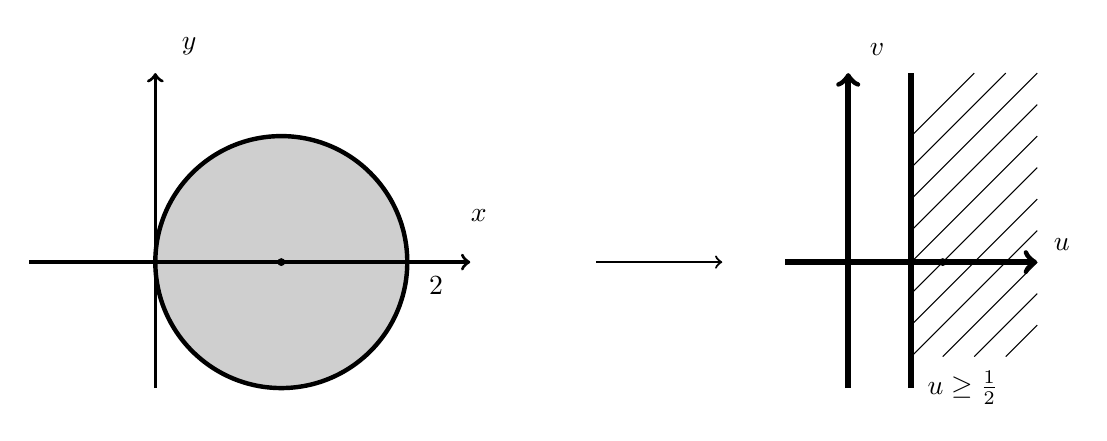
\begin{tikzpicture}[scale=0.8][line cap=round,line join=round,>=triangle 45,x=1cm,y=1cm]
				\draw [line width=1.6pt,fill=black,fill opacity=0.19] (-2,1) circle (2cm);
				\draw [->,line width=1.2pt] (-4,-1) -- (-4,4);
				\draw [->,line width=1.2pt] (-6,1) -- (1,1);
				\draw (0.19197991994709068,0.9164445322718981) node[anchor=north west] {$2$};
				\draw (8.103948156677006,-0.5763796633375331) node[anchor=north west] {$u\ge\frac{1}{2}$};
				\draw [->,line width=0.8pt] (3,1) -- (5,1);
				\draw [->,line width=2pt] (6,1) -- (10,1);
				\draw [->,line width=2pt] (7,-1) -- (7,4);
				\draw [line width=2pt] (8,-1)-- (8,4);
				\draw (-3.7320151085119515,4.712483201107309) node[anchor=north west] {$y$};
				\draw (0.8530877780026902,1.9827475291357777) node[anchor=north west] {$x$};
				\draw (10.108597790781083,1.5349002704529484) node[anchor=north west] {$u$};
				\draw (7.186927579374079,4.627178961358199) node[anchor=north west] {$v$};
				\draw [line width=0.4pt] (8,3)-- (9,4);
				\draw [line width=0.4pt] (8,2)-- (10,4);
				\draw [line width=0.4pt] (8,1)-- (10,3);
				\draw [line width=0.4pt] (8,0)-- (10,2);
				\draw [line width=0.4pt] (8,-0.5)-- (10,1.5);
				\draw [line width=0.4pt] (8.5,-0.5)-- (10,1);
				\draw [line width=0.4pt] (9,-0.5)-- (10,0.5);
				\draw [line width=0.4pt] (9.5,-0.5)-- (10,0);
				\draw [line width=0.4pt] (8,0.5)-- (10,2.5);
				\draw [line width=0.4pt] (8,1.5)-- (10,3.5);
				\draw [line width=0.4pt] (8,2.5)-- (9.5,4);
				\begin{scriptsize}
					\draw [fill=black] (-2,1) circle (1.5pt);
					\draw [fill=black] (8.5,1) circle (1.5pt);
				\end{scriptsize}
			\end{tikzpicture}
		\end{figure}

		\item $w = f(z) = \dfrac{z}{z+1}$, find the image of upper-half of unit circle. 
		
		First, $f(z) = \dfrac{z+1-1}{z+1} = 1 - \dfrac{1}{z+1}$. This is a sequence of transformations:$$z \rightarrow \underbrace{z+1}_{\text{shift right}} \rightarrow \underbrace{\dfrac{1}{z+1}}_{\text{invert}} \rightarrow \underbrace{\dfrac{-1}{z+1}}_{\text{reflect and rotate }\pi} \rightarrow \underbrace{1-\dfrac{1}{z+1}}_{\text{shift right}}$$
		\begin{figure}[H]
			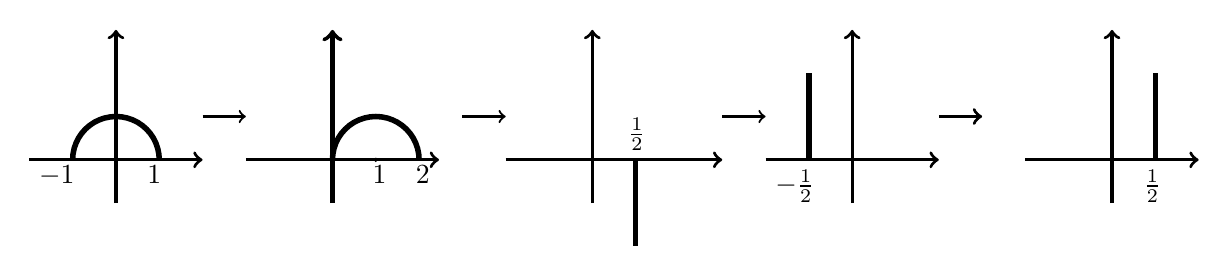
\begin{tikzpicture}[scale=0.55][line cap=round,line join=round,>=triangle 45,x=1cm,y=1cm]
				\draw [->,line width=1.2pt] (-7,0) -- (-3,0);
				\draw [->,line width=1.2pt] (-5,-1) -- (-5,3);
				\draw [->,line width=1.2pt] (-2,0) -- (2.46,0);
				\draw [->,line width=1.6pt] (0,-1) -- (0,3);
				\draw [->,line width=1.2pt] (4,0) -- (9,0);
				\draw [->,line width=1.2pt] (6,-1) -- (6,3);
				\draw [shift={(-5,0)},line width=2pt]  plot[domain=0:3.141592653589793,variable=\t]({1*1*cos(\t r)+0*1*sin(\t r)},{0*1*cos(\t r)+1*1*sin(\t r)});
				\draw [shift={(1,0)},line width=2pt]  plot[domain=0:3.141592653589793,variable=\t]({1*1*cos(\t r)+0*1*sin(\t r)},{0*1*cos(\t r)+1*1*sin(\t r)});
				\draw [->,line width=1.2pt] (10,0) -- (14,0);
				\draw [->,line width=1.2pt] (16,0) -- (20,0);
				\draw [->,line width=1.2pt] (12,-1) -- (12,3);
				\draw [->,line width=1.2pt] (18,-1) -- (18,3);
				\draw [line width=2pt] (7,0)-- (7,-2);
				\draw [line width=2pt] (11,0)-- (11,2);
				\draw [line width=2pt] (19,0)-- (19,2);
				\draw (-7,0.1) node[anchor=north west] {$-1$};
				\draw (-4.5,0.1) node[anchor=north west] {$1$};
				\draw (0.7,0.1) node[anchor=north west] {$1$};
				\draw (1.7,0.1) node[anchor=north west] {$2$};
				\draw (6.6,1.2) node[anchor=north west] {$\frac{1}{2}$};
				\draw (10,0) node[anchor=north west] {$-\frac{1}{2}$};
				\draw (18.5,0) node[anchor=north west] {$\frac{1}{2}$};
				\draw [->,line width=0.8pt] (-3,1) -- (-2,1);
				\draw [->,line width=0.8pt] (3,1) -- (4,1);
				\draw [->,line width=0.8pt] (9,1) -- (10,1);
				\draw [->,line width=1.2pt] (14,1) -- (15,1);
				\begin{scriptsize}
					\draw [fill=black] (1,0) circle (1pt);
				\end{scriptsize}
			\end{tikzpicture}
		\end{figure}
	\end{enumerate}
\end{example}
\subsection{Limits and Differentiation}
\begin{definition}
	\underline{\textbf{Limits}}: $$\lim_{z \rightarrow z_0}f(z) = w_0$$ means that for any $\epsilon > 0$, there exists $\delta > 0$ such that $$0 < |z - z_0| < \delta \;\;\; \Rightarrow \;\;\; |f(z)-w_0| < \epsilon$$
\end{definition}
\begin{example}
	Prove that $\lim_{z \rightarrow 1 + i}(2+i)z = 1+3i$.

	\underline{\textbf{Solution}}: We first do some preliminary work: $$|(2+i)z - (1+3i)| = |2+i| \cdot |z-\dfrac{1+3i}{2+i}| = \sqrt{5}\cdot |z - (1+i)|$$
	So, let $\epsilon > 0$, with $|z-z_0| < \dfrac{\epsilon}{\sqrt{5}}(= \delta)$, we have \begin{align*}
		|(2+i)z - (1+3i)| &= \sqrt{5}\cdot|z-(1+i)|\\
		&<\sqrt{5}\cdot\dfrac{\epsilon}{\sqrt{5}}\\
		&=\epsilon
	\end{align*}
	So, $\lim_{z \rightarrow 1 + i}(2+i)z = 1+3i$ \qed
\end{example}
Note that similar definitions apply when dealing with infinity, e.g. $\lim_{z \rightarrow z_0}f(z) = \infty$ means that for any $\epsilon > 0$, there exists $\delta > 0$ such that $0 < |z - z_0| < \delta \;\;\; \Rightarrow \;\;\; |f(z)| > \dfrac{1}{\epsilon}$
\begin{definition}
	\textbf{\underline{Continuity}}: $f$ is \underline{\textbf{continuous}} at $z_0$ means that $$\lim_{z \rightarrow z_0}f(z) = f(z_0)$$
\end{definition}
The usual limit and continuity theorems hold, e.g. $$\lim_{z \rightarrow z_0}f(z)g(z) = \lim_{z \rightarrow z_0}f(z) \cdot \lim_{z \rightarrow z_0}g(z)$$
\begin{theorem}
	Let $f(z) = u + iv, z_0 = x_0 + iy_0, w_0 = u_0 + iv_0$, then $$\lim_{z \rightarrow z_0} f(z) = w_0 \;\;\text{ if and only if }\;\; \begin{dcases}
		\lim_{(x,y) \rightarrow (x_0, y_0)} u(x, y) = u_0\\
		\lim_{(x,y) \rightarrow (x_0, y_0)} v(x, y) = v_0
	\end{dcases}$$
\end{theorem}
\begin{definition}
	\underline{\textbf{Differentiation}}: $$f'(z_0) = \lim_{z \rightarrow z_0} \dfrac{f(z)-f(z_0)}{z - z_0} \bigg(= \lim_{\Delta z \rightarrow 0} \dfrac{f(z_0 + \Delta z) - f(z_0)}{\Delta z}\bigg)$$
	Derivative function is $$f'(z)= \lim_{\Delta z \rightarrow 0} \dfrac{f(z + \Delta z) - f(z)}{\Delta z}$$
\end{definition}
For functions with real analogues (e.g. $f(z) = z^2$ analogous to $f(x) = x^2$), the usual rules (power, quotient, etc.) apply, e.g. $$f(z) = 3z^2+z^4 \;\; \Rightarrow f'(z) = 6z+4z^3$$

What about functions without real analogues? 
\begin{example}
	$f(z) = \overline{z}$. Is it differentiable? 

	\textbf{\underline{Solution}}: 
	\begin{align*}
		f'(z_0) &= \lim_{z \rightarrow z_0}\dfrac{\overline{z} - \overline{z_0}}{z-z_0}\\
		&=\lim_{z \rightarrow z_0} \dfrac{\overline{z-z_0}}{z-z_0}\\
		&=\lim_{z \rightarrow z_0} \dfrac{\overline{re^{i\theta}}}{re^{i\theta}} \;\;\text{ where }\;\; z-z_0 = e^{i\theta}\\
		&=\lim_{z \rightarrow z_0} \dfrac{e^{-i\theta}}{e^{i\theta}}\\
		&=\lim_{z \rightarrow z_0} e^{-i2\theta}
	\end{align*}
	which depends on $\theta$! No unique value, so limit DNE. So, $f$ is not differentiable anywhere. 
\end{example}
\begin{theorem}
	\underline{\textbf{Cauchy-Riemann Equations}}: If $f(z) = u(x,y) + iv(x,y)$ and $f'(z_0)$ exists, then 
	\begin{tcolorbox}[hbox, before=\par\smallskip\centering]
		$u_x = v_y\;\;$ and $\;\;v_x = -u_y$ $\;\;\;\;\;$ at $(x_0, y_0)$
	\end{tcolorbox}
	Note that for notation, \begin{align*}
		u_x &= \dfrac{\partial u}{\partial x}\\
		u_y &= \dfrac{\partial u}{\partial y}\\
		v_x &= \dfrac{\partial v}{\partial x}\\
		v_y &= \dfrac{\partial v}{\partial y}
	\end{align*}
\end{theorem}
\begin{proof}
	\begin{align*}
		f'(z_0) &= \lim_{\Delta z \rightarrow 0} \dfrac{f(z_0 + \Delta z) - f(z_0)}{\Delta z}\\
		&= \lim_{(\Delta x, \Delta y)  \rightarrow (0, 0)} \bigg( \dfrac{u(x_0 + \Delta x, y_0 + \Delta y) - u(x_0, y_0)}{\Delta x + i \Delta y} + i \dfrac{v(x_0 + \Delta x, y_0 + \Delta y) - v(x_0, y_0)}{\Delta x + i \Delta y} \bigg)
	\end{align*}
	Since the limit exists, it must be independent of path, so \begin{itemize}
		\item Along $\Delta y = 0$: $$f'(z_0) = \lim_{\Delta x \rightarrow 0} \dfrac{u(x_0 + \Delta x, y_0) - u(x_0, y_0)}{\Delta x} + i (\cdots) = \dfrac{\partial u}{\partial x} + i \dfrac{\partial v}{\partial x}$$
		\item Along $\Delta x = 0$: $$f'(z_0) = \lim_{\Delta y \rightarrow 0} \dfrac{u(x_0, y_0+\Delta y) - u(x_0, y_0)}{i\Delta y} + i (\cdots) = -i \dfrac{\partial u}{\partial y} + \dfrac{\partial v}{\partial y}$$
	\end{itemize}
	Equating the real and imaginary part yields the result. 
\end{proof}
\subsection{Differentiability Continued}
\begin{example}
	Is $f(z) = |z|^2$ differentiable? Where? 

	\textbf{\underline{Solution}}: $f(z) = \sqrt{x^2+y^2}^2 = \underbrace{x^2+y^2}_{u} + \underbrace{0}_{v}i$. So, by CRE, we know that $\begin{dcases}
		u_x = v_y & \Rightarrow 2x = 0\\
		v_x = -u_y & \Rightarrow 0 = -2y
	\end{dcases}$

	It's clear that this is satisfied only at $x=y=0$. 

	So, if $(x,y) \neq (0,0)$, i.e. $z \neq 0$, then $f$ is not differentiable. 

	When $z = 0$, $f'(z) = \lim_{\Delta z \rightarrow 0}\dfrac{f(0 + \Delta z) - f(0)}{\Delta z} = \lim_{\Delta z \rightarrow 0} \dfrac{|\Delta z|^2 - 0}{\Delta z} = 0$. This is because $\bigg|\dfrac{|\Delta z|^2}{\Delta z} - 0\bigg| \leq |\Delta z| \rightarrow 0$ as $\Delta z \rightarrow 0$ (by applying the squeeze theorem).  
\end{example}
Hence, CRE are necessary but not sufficient conditions. 
\begin{theorem}
	Let $f$ be defined in some neighborhood of $z_0$. If $u_x, u_y, v_x, v_y$ exist in that neighborhood, satisfying CRE at $z_0$, and are \underline{\textbf{continuous}} at $z_0$, then $f$ is differentiable at $z_0$. 
\end{theorem}
\begin{definition}
	$f(z)$ is \underline{\textbf{analytic at $z_0$}} if $f'(z)$ exists at every point in some neighborhood of $z_0$. 
	
	$f(z)$ is \underline{\textbf{analytic on an open set $S$}} if it is analytic at every point of $S$. 
\end{definition}
\begin{example}
	$f(z) = z^3 = \cdots =\underbrace{(x^3-3xy^2)}_{u(x,y)} + i\underbrace{(3x^2y-y^2)}_{v(x,y)}$.

	We have \begin{align*}
		u_x &= 3x^2-3y^2\\
		u_y &= -6xy\\
		v_x &= 6xy\\
		v_y &= 3x^2-3y^2
	\end{align*}
	So, CRE satisfied everywhere. All partial derivatives are continuous. By theorem, $f$ is differentiable everywhere, so is analytic everywhere. We refer to ``analytic everywhere'' as ``entire''
\end{example}
\begin{example}
	Where is $f(z) = x^2+iy^2$ analytic? 

	We have \begin{align*}
		u_x &= 2x\\
		u_y &= 0\\
		v_x &= 0\\
		v_y &= 2y
	\end{align*}
	We need $x=y$ to satisfy CRE. 
	\begin{itemize}
		\item If $x \neq y$, $f$ is not differentiable, so not analytic. 
		\item If $x = y$, $f$ cannot be analytic because we are not on an open set. 
	\end{itemize}
	So, $f$ is not analytic nowhere. 
\end{example}
\begin{theorem}
	Sums, products, and compositions of analytic functions are also analytic, except when $\div 0$
\end{theorem}
\begin{example}
	$f(z) = \dfrac{z^3+2}{z^2+1}$ is analytic everywhere except at $z = \pm i$.

	$g(z) = f(z^2)$ is analytic everywhere except wherre $z^2 = \pm i$, i.e. except \begin{align*}
		z &= e^{i (\dfrac{n\pi + \pi / 2}{2})}\\
		&= e^{i (n\pi / 2 + \pi / 4)}\\
		&= e^{i (n\pi/4)}, e^{i (n3\pi/4)}, e^{i (n5\pi/4)}, e^{i (n7\pi/4)}\\
		&=\dfrac{1}{\sqrt{2}}+ \dfrac{i}{\sqrt{2}}, -\dfrac{1}{\sqrt{2}}+ \dfrac{i}{\sqrt{2}}, -\dfrac{1}{\sqrt{2}} - \dfrac{i}{\sqrt{2}},\dfrac{1}{\sqrt{2}} - \dfrac{i}{\sqrt{2}},
	\end{align*}
\end{example}
\begin{theorem}
	Suppose $f$ is analytic in a domain $D$. If $f'(z) = 0$ for all $z \in D$, then $f$ is constant in $D$
\end{theorem}
\begin{proof}
	$f'(z) = u_x + iv_x = v_y - iu_y$. So, $f'(z) = 0 \Rightarrow u_x = v_y = 0 = v_y = u_y$. So, $u$ and $v$ are constant, since $D$ is connected. 
\end{proof}
\begin{theorem}
	Suppose $f$ is analytic in a domain $D$. If $|f(z)| = M$ for all $z \in D$, where $M$ is constant, then $f(z)$ is constant in $D$. 
\end{theorem}
\begin{proof}
	$|f(z)|^2 = u^2 + v^2 = M^2$. 

	We differentiate: \begin{itemize}
		\item with respect to $x$: $2uu_x + 2vv_x = 0$ $\;\;$-- (1)
		\item with respect to $y$: $2uu_y + 2vv_y = 0$ $\;\;$-- (2)
	\end{itemize}
	Now $u_x = v_y$, and $v_x = -u_y$, so the (2) gives $-uv_x + vu_x = 0$ $\;\;$-- (3). 

	Multiply (1) by $u_x$. \begin{align*}
		&\;\;\; uu_x^2 + vu_xv_x = 0\\
		& \Rightarrow \; uux^2 + (uv_x)v_x = 0 \;\;\text{ by (3)}\\
		& \Rightarrow \; u(u_x^2+v_x^2) = 0
	\end{align*}
	So, unless $u = 0$ for all $z \in D$, we must have $u_x^2 + v_x^2 = 0$. So, $u_x = v_x = 0$, implying that $u, v$ are constant. Hence, $f$ is constant. 

	What if $u = 0$ for all $z \in D$? Then, $u_x = u_y = 0$, so $v_x = v_y = 0$ by CRE. $f$ is constant as well. 
\end{proof}
\subsection{Harmonic Functions}
Recap: $$f'(z) = u_x + iv_x = \dfrac{u_y+iv_y}{i} = v_y - iu_y$$
$$CRE: \;\;\; u_x = v_y \;\;\;\; v_x = -u_y$$
Also, ``analytic'' means differentiable on a open set. 

Suppose $f(z) = u(x,y) + iv(x,y)$ is analytic in a domain $D$. Then $u$ and $v$ satisfy CRE. 

Also, which will be shown later, $u, v \in C^2$ (continuous under second partial derivatives), and this implies that $u_{xy} = u_{yx}$, and $v_{xy} = v_{yx}$. 

From CRE: $$\underbrace{u_x- v_y}_{\Rightarrow \; u_{xx} = v_{yx}} \;\;\;\; \text{ and } \;\;\;\; \underbrace{v_x = -u_y}_{\Rightarrow \; u_{yy} = -v_{xy}}$$

\begin{definition}
	From the above derivation, we see $$u_{xx}+u_{yy} = v_{yx} - v_{xy} = 0$$ and $$v_{xx} + v_{yy} = 0$$

	We refer to these as \underline{\textbf{``Laplace's equation''}}

	Solution to Laplace's equation are called \underline{\textbf{``harmonic functions''}}
\end{definition}
Notes: \begin{itemize}
	\item We've shown that if $f(z) = u+iv$ is analytic, then $u$ and $v$ must be harmonic
	\item Laplace's equation is very useful! We will see that later. 
	\item $u_{xx} + u_{yy} = 0$ is also denoted as $\Delta^2 u = 0$, and we denote $\Delta$ as ``Laplacian operator''.  
\end{itemize}
\begin{example}
	Suppose $u(x,y) = e^{-2x}\cos 2y + 2y$. Find $v(x,y)$ such that $f(z) = u+iv$ is analytic. 
	
	\underline{\textbf{Solution}}: $u$ and $v$ must satisfy CRE. So, $v_y = u_x = -2e^{-2x}\cos 2y$. Hence, \begin{align*}
		v &= \int -2e^{-2x}\cos 2y dy\\
		&=-e^{2x}\sin 2y +C(x) 
	\end{align*}
	Note that $C(x)$ is a function of all other variables. 
	
	Now we try to make it satisfy other CRE: \begin{align*}
		v_x = -u_y \; &\Rightarrow \; 2e^{-2x}\sin 2y + C'(x) = 2e^{-2x}\sin 2y -2 \\
		&\Rightarrow \; C'(x) = -2\\
		&\Rightarrow \; C(x) = -2x+k
	\end{align*}
	Therefore, $v(x,y) = -e^{-2x}\sin 2y -2x + k$
\end{example}

Note that $v(x,y)$ is called the ``harmonic conjugate'' of $u$. 

Exercise: show that if $v$ is the harmonic conjugate of $u$, then $-u$ is the harmonic conjugate of $v$. 

\begin{example}
	Solve Laplace's equation $\Phi_{xx} + \Phi_{yy} = 0$ on region between hyperbolas $x^2 - y^2 = 1$ and $x^2 - y^2 = 4$, $x > 0$, with ``boundary conditions'' $$\begin{dcases}
		\Phi = 0 & \text{on }x^2-y^2 = 1\\
		\Phi = 10 & \text{on }x^2-y^2 = 4
	\end{dcases}$$
	i.e. Find $\Phi(x, y)$

	\begin{center}
		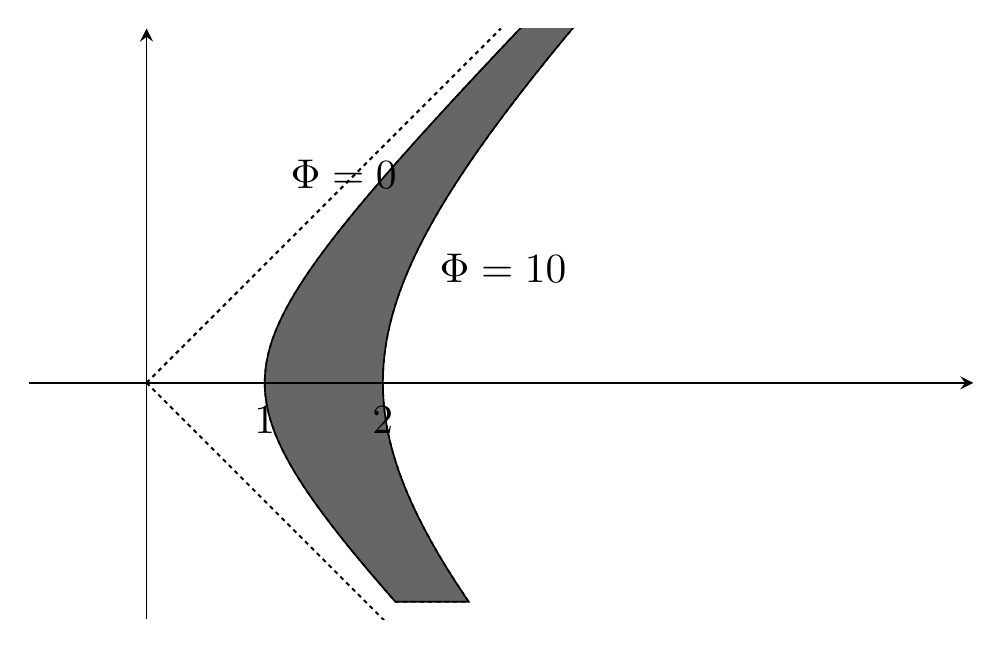
\begin{tikzpicture}[scale=1.5]
			\begin{axis}[
				x=1cm,y=1cm,
				axis lines=middle,
				xmin=-1,
				xmax=7,
				ymin=-2,
				ymax=3,
				xtick={0,1,2},
				ytick=\empty,]
				\draw[line width=0.4pt,dash pattern=on 1pt off 1pt,fill=black,fill opacity=0.37](3.274662080624353,3.11793063089423)--(3.078142092260624,2.9111782391579215)--(2.8331024958925553,2.65074890403309)--(2.62235876612791,2.424204095840096)--(2.439457643220119,2.2250738399129717)--(2.2794823017751518,2.04842367788164)--(2.1386215920525538,1.8904238450658102)--(2.013876570275504,1.7480557314641392)--(1.902855849728697,1.6189071575747387)--(1.8036299216591194,1.5010266134562968)--(1.7146255358809155,1.3928175502537714)--(1.6345478583034294,1.2929604406494146)--(1.5623222466932392,1.2003544486994708)--(1.4970501151013949,1.1140731785323166)--(1.4379750703709617,1.0333306842479673)--(1.3844566424842901,0.9574550615662721)--(1.3359497007199626,0.8858677118248286)--(1.2919881773739395,0.818066898532164)--(1.2521720907696334,0.7536145864448188)--(1.2161571212858309,0.692125814902348)--(1.1836461820996187,0.6332600448465099)--(1.154382562835803,0.5767140551255507)--(1.1281443245617162,0.5222160635606788)--(1.1047396989865015,0.4695208222398513)--(1.0840033005398864,0.41840549181549586)--(1.0657930022854967,0.36866614127247027)--(1.0499873589659243,0.3201147512818441)--(1.0364834854637945,0.27257662342757116)--(1.025195318469489,0.22588811613663334)--(1.0160522045474452,0.1798946424041676)--(1.0089977701103137,0.1344488753675005)--(1.0039890388117536,0.08940911616915155)--(1.0009957701407863,0.044637784888429025)--(1,0)--(1.0009957701407863,-0.044637784888429025)--(1.0039890388117536,-0.08940911616915155)--(1.0089977701103137,-0.1344488753675005)--(1.0160522045474452,-0.1798946424041676)--(1.025195318469489,-0.22588811613663334)--(1.0364834854637945,-0.27257662342757116)--(1.0499873589659243,-0.3201147512818441)--(1.0657930022854967,-0.36866614127247027)--(1.0840033005398864,-0.41840549181549586)--(1.1047396989865015,-0.4695208222398513)--(1.1281443245617162,-0.5222160635606788)--(1.154382562835803,-0.5767140551255507)--(1.1836461820996187,-0.6332600448465099)--(1.2161571212858309,-0.6921258149023477)--(1.2521720907696334,-0.7536145864448188)--(1.2919881773739395,-0.8180668985321636)--(1.3359497007199626,-0.8858677118248286)--(1.3844566424842901,-0.9574550615662718)--(1.4379750703709617,-1.0333306842479673)--(1.4970501151013949,-1.1140731785323166)--(1.5623222466932392,-1.2003544486994708)--(1.6345478583034294,-1.2929604406494148)--(1.7146255358809155,-1.392817550253771)--(1.8036299216591194,-1.501026613456297)--(1.902855849728697,-1.6189071575747385)--(2.013876570275504,-1.7480557314641394)--(2.106493985617573,-1.853757478283976)--(2.7272960359541996,-1.853757478283976)--(2.705031186697621,-1.8213164801886406)--(2.6215420882179234,-1.6948400869397646)--(2.545247951175891,-1.5742576450394234)--(2.475585301839686,-1.4589457106707866)--(2.4120621868658976,-1.3483486171270012)--(2.354248395352079,-1.241968400168796)--(2.3017673458053984,-1.1393563596241645)--(2.2542893280972573,-1.040105944013966)--(2.2115258561439055,-0.943846710219957)--(2.1732249376845645,-0.8502391603390652)--(2.1391671068871294,-0.7589702966439806)--(2.1091620963576054,-0.6697497657421086)--(2.0830460495047594,-0.5823064866179866)--(2.0606791936405027,-0.4963856757631847)--(2.0419439098274945,-0.41174619716713284)--(2.0267431481919322,-0.3281581764072716)--(2.0149991478729583,-0.24540082707429625)--(2.0066524295027275,-0.16326044477827598)--(2.0016610355153692,-0.08152852936525122)--(2,0)--(2.0016610355153692,0.08152852936525122)--(2.0066524295027275,0.16326044477827598)--(2.0149991478729583,0.24540082707429625)--(2.0267431481919322,0.3281581764072716)--(2.0419439098274945,0.41174619716713284)--(2.0606791936405027,0.4963856757631847)--(2.0830460495047594,0.5823064866179866)--(2.1091620963576054,0.6697497657421086)--(2.1391671068871294,0.7589702966439806)--(2.1732249376845645,0.8502391603390652)--(2.2115258561439055,0.943846710219957)--(2.2542893280972573,1.040105944013966)--(2.3017673458053984,1.1393563596241647)--(2.354248395352079,1.241968400168796)--(2.4120621868658976,1.3483486171270014)--(2.475585301839686,1.4589457106707866)--(2.545247951175891,1.5742576450394234)--(2.6215420882179234,1.6948400869397648)--(2.705031186697621,1.8213164801886406)--(2.796362079425364,1.9543901553293148)--(2.8962793668882174,2.094858985961207)--(3.005643055848226,2.2436332541591244)--(3.1254502909692925,2.4017575900411)--(3.2568623181918555,2.570438126012377)--(3.401238197238152,2.751076384681428)--(3.560177306884961,2.945311945526085)--(3.704513524284938,3.11793063089423);
				\draw[line width=0.4pt,fill=black,fill opacity=0.37](3.274662080624353,3.11793063089423)--(3.078142092260624,2.9111782391579215)--(2.8331024958925553,2.65074890403309)--(2.62235876612791,2.424204095840096)--(2.439457643220119,2.2250738399129717)--(2.2794823017751518,2.04842367788164)--(2.1386215920525538,1.8904238450658102)--(2.013876570275504,1.7480557314641392)--(1.902855849728697,1.6189071575747387)--(1.8036299216591194,1.5010266134562968)--(1.7146255358809155,1.3928175502537714)--(1.6345478583034294,1.2929604406494146)--(1.5623222466932392,1.2003544486994708)--(1.4970501151013949,1.1140731785323166)--(1.4379750703709617,1.0333306842479673)--(1.3844566424842901,0.9574550615662721)--(1.3359497007199626,0.8858677118248286)--(1.2919881773739395,0.818066898532164)--(1.2521720907696334,0.7536145864448188)--(1.2161571212858309,0.692125814902348)--(1.1836461820996187,0.6332600448465099)--(1.154382562835803,0.5767140551255507)--(1.1281443245617162,0.5222160635606788)--(1.1047396989865015,0.4695208222398513)--(1.0840033005398864,0.41840549181549586)--(1.0657930022854967,0.36866614127247027)--(1.0499873589659243,0.3201147512818441)--(1.0364834854637945,0.27257662342757116)--(1.025195318469489,0.22588811613663334)--(1.0160522045474452,0.1798946424041676)--(1.0089977701103137,0.1344488753675005)--(1.0039890388117536,0.08940911616915155)--(1.0009957701407863,0.044637784888429025)--(1,0)--(1.0009957701407863,-0.044637784888429025)--(1.0039890388117536,-0.08940911616915155)--(1.0089977701103137,-0.1344488753675005)--(1.0160522045474452,-0.1798946424041676)--(1.025195318469489,-0.22588811613663334)--(1.0364834854637945,-0.27257662342757116)--(1.0499873589659243,-0.3201147512818441)--(1.0657930022854967,-0.36866614127247027)--(1.0840033005398864,-0.41840549181549586)--(1.1047396989865015,-0.4695208222398513)--(1.1281443245617162,-0.5222160635606788)--(1.154382562835803,-0.5767140551255507)--(1.1836461820996187,-0.6332600448465099)--(1.2161571212858309,-0.6921258149023477)--(1.2521720907696334,-0.7536145864448188)--(1.2919881773739395,-0.8180668985321636)--(1.3359497007199626,-0.8858677118248286)--(1.3844566424842901,-0.9574550615662718)--(1.4379750703709617,-1.0333306842479673)--(1.4970501151013949,-1.1140731785323166)--(1.5623222466932392,-1.2003544486994708)--(1.6345478583034294,-1.2929604406494148)--(1.7146255358809155,-1.392817550253771)--(1.8036299216591194,-1.501026613456297)--(1.902855849728697,-1.6189071575747385)--(2.013876570275504,-1.7480557314641394)--(2.106493985617573,-1.853757478283976)--(2.7272960359541996,-1.853757478283976)--(2.705031186697621,-1.8213164801886406)--(2.6215420882179234,-1.6948400869397646)--(2.545247951175891,-1.5742576450394234)--(2.475585301839686,-1.4589457106707866)--(2.4120621868658976,-1.3483486171270012)--(2.354248395352079,-1.241968400168796)--(2.3017673458053984,-1.1393563596241645)--(2.2542893280972573,-1.040105944013966)--(2.2115258561439055,-0.943846710219957)--(2.1732249376845645,-0.8502391603390652)--(2.1391671068871294,-0.7589702966439806)--(2.1091620963576054,-0.6697497657421086)--(2.0830460495047594,-0.5823064866179866)--(2.0606791936405027,-0.4963856757631847)--(2.0419439098274945,-0.41174619716713284)--(2.0267431481919322,-0.3281581764072716)--(2.0149991478729583,-0.24540082707429625)--(2.0066524295027275,-0.16326044477827598)--(2.0016610355153692,-0.08152852936525122)--(2,0)--(2.0016610355153692,0.08152852936525122)--(2.0066524295027275,0.16326044477827598)--(2.0149991478729583,0.24540082707429625)--(2.0267431481919322,0.3281581764072716)--(2.0419439098274945,0.41174619716713284)--(2.0606791936405027,0.4963856757631847)--(2.0830460495047594,0.5823064866179866)--(2.1091620963576054,0.6697497657421086)--(2.1391671068871294,0.7589702966439806)--(2.1732249376845645,0.8502391603390652)--(2.2115258561439055,0.943846710219957)--(2.2542893280972573,1.040105944013966)--(2.3017673458053984,1.1393563596241647)--(2.354248395352079,1.241968400168796)--(2.4120621868658976,1.3483486171270014)--(2.475585301839686,1.4589457106707866)--(2.545247951175891,1.5742576450394234)--(2.6215420882179234,1.6948400869397648)--(2.705031186697621,1.8213164801886406)--(2.796362079425364,1.9543901553293148)--(2.8962793668882174,2.094858985961207)--(3.005643055848226,2.2436332541591244)--(3.1254502909692925,2.4017575900411)--(3.2568623181918555,2.570438126012377)--(3.401238197238152,2.751076384681428)--(3.560177306884961,2.945311945526085)--(3.704513524284938,3.11793063089423);
				\draw [line width=0.5pt,dash pattern=on 1pt off 1pt] (0,0)-- (3,3);
				\draw [line width=0.5pt,dash pattern=on 1pt off 1pt] (0,0)-- (3,-3);
				\draw (1.0948081886474288,2.0078399652952794) node[anchor=north west] {$\Phi=0$};
				\draw (2.3567061247556373,1.210851795121674) node[anchor=north west] {$\Phi=10$};
			\end{axis}
		\end{tikzpicture}
	\end{center}

	\underline{\textbf{Solution}}: Consider $f(z) = z^2 = (x+yi)^2 = \underbrace{x^2-y^2}_{u(x,y)} + i\underbrace{2xy}_{v(x,y)}$

	Since $f(z)$ is already analytic, we have that $u(x,y) = x^2-y^2$ is harmonic. Boundary curves of region are level curves of a harmonic function. 

	Is the solution $\Phi(x,y) = x^2-y^2$? No. 

	Try $\Phi(x, y) = A\cdot (x^2-y^2)+B$ (also harmonic by linearity). 

	Applying the Boundary Conditions: \begin{align*}
		0 = A \cdot 1 + B & \Rightarrow \; B = -A\\
		10 = A \cdot 4 + B & \Rightarrow \; A = \dfrac{10}{3}, B = -\dfrac{10}{3}
	\end{align*}
	So the solution is $\Phi(x,y) = \dfrac{10}{3}(x^2-y^2)-\dfrac{10}{3}$
\end{example}
Notes: \begin{itemize}
	\item It can be used in temperature distribution
	\item What about more complicated regions? 
	\item Orthogonal trajectories
	\begin{center}
		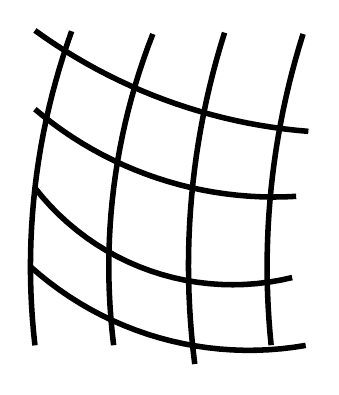
\begin{tikzpicture}
			\draw [shift={(2.7532914746964243,1)},line width=2pt]  plot[domain=2.7953545897816907:3.2553422400667853,variable=\t]({1*8.810227672483448*cos(\t r)+0*8.810227672483448*sin(\t r)},{0*8.810227672483448*cos(\t r)+1*8.810227672483448*sin(\t r)});
			\draw [shift={(3.0271301929022627,1)},line width=2pt]  plot[domain=2.76757136404437:3.2655316496383815,variable=\t]({1*8.08917913844187*cos(\t r)+0*8.08917913844187*sin(\t r)},{0*8.08917913844187*cos(\t r)+1*8.08917913844187*sin(\t r)});
			\draw [shift={(5.74915387214404,1.0113464410519617)},line width=2pt]  plot[domain=2.834591536362894:3.269482313515557,variable=\t]({1*9.799154916744698*cos(\t r)+0*9.799154916744698*sin(\t r)},{0*9.799154916744698*cos(\t r)+1*9.799154916744698*sin(\t r)});
			\draw [shift={(6.749743314584557,1)},line width=2pt]  plot[domain=2.835272950547197:3.2438020438334467,variable=\t]({1*9.800892546104476*cos(\t r)+0*9.800892546104476*sin(\t r)},{0*9.800892546104476*cos(\t r)+1*9.800892546104476*sin(\t r)});
			\draw [shift={(-1.987135331002164,9.525729337995672)},line width=2pt]  plot[domain=4.084285192044407:4.633375921958299,variable=\t]({1*6.829111770096987*cos(\t r)+0*6.829111770096987*sin(\t r)},{0*6.829111770096987*cos(\t r)+1*6.829111770096987*sin(\t r)});
			\draw [shift={(-2.965009369560112,6.569981260879775)},line width=2pt]  plot[domain=4.007812545169585:4.773068445264867,variable=\t]({1*4.68571598903419*cos(\t r)+0*4.68571598903419*sin(\t r)},{0*4.68571598903419*cos(\t r)+1*4.68571598903419*sin(\t r)});
			\draw [shift={(-3.4892419868854327,3.9479739763179724)},line width=2pt]  plot[domain=3.801434135672984:4.952857222143927,variable=\t]({1*3.1778150375424716*cos(\t r)+0*3.1778150375424716*sin(\t r)},{0*3.1778150375424716*cos(\t r)+1*3.1778150375424716*sin(\t r)});
			\draw [shift={(-3.280269756608991,4.0959324511562984)},line width=2pt]  plot[domain=3.9813027208426544:4.88633150707663,variable=\t]({1*4.158686603687145*cos(\t r)+0*4.158686603687145*sin(\t r)},{0*4.158686603687145*cos(\t r)+1*4.158686603687145*sin(\t r)});
		\end{tikzpicture}
	\end{center}
	\item list of harmonic functions
\end{itemize}

\section{Elementary Functions}
\subsection{Elementary Functions}
\begin{definition}
	\underline{\textbf{Polynomials}}: 
	$$p(z) = a_0 + a_1z + a_2z^2 + \cdots + a_nz^n \;,\;\;\; a_i\in \mathbb{C}$$
	There are obviously \underline{\textbf{entire}}. 

	The fundamental theorem of algebra guarantees that we can factor this as $$p(z) = a_n(z-z_1)(z-z_2) \cdots (z-z_n)$$
	Note that $z_i$ are not necessarily distinct. 

	$z_0$ is a ``zero of multiplicity'' $k$ if and only if $$p(z) = (z - z_0)^kq(z)$$ where $q(z)$ is a polynomial such that $q(z_0) \neq 0$
\end{definition}
\begin{definition}
	\underline{\textbf{Rational Functions}}: 
	$$R(z) = \dfrac{p(z)}{q(z)} = \dfrac{a_n(z-z_1)(z-z_2)\cdots(z-z_n)}{b_m(z-w_1)(z-w_2)\cdots (z-w_n)}$$
	Suppose all common factors have been cancelled, then \begin{itemize}
		\item the roots (or zeroes) of $p(z)$ are called the \underline{\textbf{roots/zeroes}} of $R(z)$
		\item the roots (or zeroes) of $q(z)$ are called the \underline{\textbf{poles}} of $R(z)$
	\end{itemize}
\end{definition}
\begin{example}
	$$R(z) = \dfrac{3i(z-1)(z-\frac{1}{3}i)^2(z+i)}{(z-i)^3(z-2-i)}$$
	Zeroes at 1 and $-i$ (order 1 would be a ``simple zero''), and $\dfrac{1}{3}i$ (order 2). 

	Poles at $i$ (order 3) and $2+i$ (order 1 would be a ``simple pole'')
\end{example}
Partial Fractions has simpler rules: 
\begin{example}
	Decompose $R(z) = \dfrac{1}{(z+4)^2(z^2+1)}$

	\underline{\textbf{Solution}}: Factor and expand $$\dfrac{1}{(z+4)^2(z^2+1)} = \dfrac{A}{z+4} + \dfrac{B}{(z+4)^2} + \dfrac{C}{z+i}+\dfrac{D}{z-i}$$
	This gives us $$1 = A\cdot (z+4)(z+i)(z-i) + B(z+i)(z-i) + C(z+4)^2(z-i) + D(z+4)^2(z+i)$$
	We can solve this by: \begin{itemize}
		\item set $z = -4$, this gives us $1 = 0 + (-4+i)(-4-i)B +0+0$, so $B = \dfrac{1}{17}$
		\item set $z = -i$, this gives us $1 = 0 + 0 + (-i+4)^2(-2i)C +0$. Then we conpute $(-2i)(15-8i) = 16-30i$, also $(-16-30i) = \dfrac{(-16-30i)(-16+30i)}{(-16+30i)} = \dfrac{1156}{(-16+30i)} = \dfrac{578}{-8+15i}$. 
		
		Hence, $C = \dfrac{-8+15i}{578}$. 
		\item set $z = -4$, this gives us $1 = 0 + 0+0+ (i+4)^2(2i)D$, so $D = \dfrac{-8-15i}{578}$. The trick to compute things here is that, we can replace $i$ with $-i$ from $C$ since the expression is similar to $C$. 
	\end{itemize}
	Now what about $A$? We can try another $z$, or just compare the coefficients of $z^3$. By comparing the coefficients of $z^3$, we get that $$0 + A + C + D = A + \dfrac{-8+15i}{578} + \dfrac{-8-15i}{578}$$ So $A = \dfrac{16}{578} = \dfrac{8}{289}$

	Hence, $$\dfrac{1}{(z+4)^2(z^2+1)} = \dfrac{8/289}{z+4} +\dfrac{1/17}{(z+4)^2} + \dfrac{\frac{-8+15i}{578}}{z+i}+\dfrac{\frac{-8-15i}{578}}{z-i}$$
\end{example}
Actually, often we will only need one of the coefficients, and there's a quick way which will be covered later in the course. 
\begin{definition}
	\underline{\textbf{Exponential Function}}: We already defined that $e^z = e^{x+iy} = e^x(\cos y + i\sin y)$. 

	Note that $e^{z_1+z_2} = e^{z_1}e^{z_2}$, $\dfrac{d}{dz} e^z= e^z$. Also, $e^z$ is \underline{\textbf{periodic}} with period $2\pi i$
\end{definition}
\begin{definition}
	\underline{\textbf{Hyperbolic Functions}}: From real calculus, we seen that \begin{align*}
		\cosh x &= \dfrac{1}{2}(e^x+e^{-x}) \;\;\;\text{ this is the even component of }e^x\\
		\sinh x &= \dfrac{1}{2}(e^x-e^{-x}) \;\;\;\text{ this is the odd component of }e^x
	\end{align*}
	It can be shown that \begin{align*}
		&\cosh x + \sinh x = e^x\\
		&\cosh^2 x - \sinh^2 x = 1\\
		&\dfrac{d}{dx} \sinh x = \cosh x\\
		&\dfrac{d}{dx} \cosh x = \sinh x
	\end{align*}
	\begin{center}
		\begin{tikzpicture}
			\begin{axis}[
				axis lines = middle,
				xlabel = $x$,
				ylabel = {$y$},
				xtick=\empty,
				ytick=\empty,
				legend style={at={(1.5,0.5)},anchor=south east}
				]
				\addplot [
				domain=-1:1, 
				samples y = 0,
				color=blue,
				]
				{cosh(x)};
				\addlegendentry{$\cosh(x)$}
				\addplot [
				domain=-1:1, 
				samples y = 0, 
				color=red
				]
				{0.5*e^x};
				\addlegendentry{$\frac{e^x}{2}$}
				\addplot [
				domain=-1:1, 
				samples y = 0, 
				color = brown
				]
				{0.5*e^(-x)};	
				\addlegendentry{$-\frac{e^x}{2}$}
			\end{axis}
		\end{tikzpicture}
		
		\begin{tikzpicture}
			\begin{axis}[
				axis lines = middle,
				xlabel = $x$,
				ylabel = {$y$},
				xtick=\empty,
				ytick=\empty,
				legend style={at={(1.5,0.5)},anchor=south east}
				]
				\addplot [
				domain=-2:2, 
				samples y = 0,
				color=blue,
				]
				{sinh(x)};
				\addlegendentry{$\sinh(x)$}
				\addplot [
				domain=-2:2, 
				samples y = 0, 
				color=red,
				]
				{0.5*e^x};
				\addlegendentry{$\frac{e^{x}}{2}$}
				\addplot [
				domain=-2:2, 
				samples y = 0, 
				color=brown,
				]
				{-0.5*e^(-x)};
				\addlegendentry{$-\frac{e^{-x}}{2}$}	
			\end{axis}
		\end{tikzpicture}
	\end{center}
	To extend these to $\mathbb{C}$, we define 
	\begin{tcolorbox}[hbox, before=\par\smallskip\centering]
		$\cosh z = \dfrac{1}{2}(e^z+e^{-z}) \;\;\; \sinh z = \dfrac{1}{2}(e^z-e^{-z})$
	\end{tcolorbox}
\end{definition}
\subsection{Trigonometric and Logarithmic Function}
\begin{definition}
	\underline{\textbf{Trigonometric Functions}}: Recall \begin{align*}
		e^{i\theta} &= \cos \theta + i\sin \theta\\
		e^{-i\theta} &= \cos \theta - i\sin \theta
	\end{align*}
	Sum to get $\cos \theta = \dfrac{e^{i\theta} + e^{-i\theta}}{2}$, and $\cos \theta = \dfrac{e^{i\theta} - e^{-i\theta}}{2i}$

	We define \begin{tcolorbox}[hbox, before=\par\smallskip\centering]
		$\cos z = \dfrac{1}{2}(e^{iz}+e^{-iz})= \cosh (iz) \;\;\; \sin z = \dfrac{1}{2i}(e^{iz}-e^{-iz}) = \dfrac{1}{i}\sinh (iz)$
	\end{tcolorbox}
\end{definition}
Furthermore: \begin{align*}
	\cos(iz) &= \dfrac{e^{-z}+e^z}{2} = \cosh z\\
	\sin(iz) &= \dfrac{e^{-z}-e^z}{2i} = i\sinh z
\end{align*}
\begin{align*}
	\text{ For real }z,\;\;\; e^z &= e^x = \cosh x + \sinh x\\
	\text{ For imaginary }z,\;\;\; e^z &= e^{iy} = \cos y + i\sin y
\end{align*}
The $\cosh x$ and $\cos y$ are the even parts, and $\sinh x$ and $i\sin y$ are the odd parts
\begin{center}
	\begin{tabular}{c|c|c}
		Functions & Along Real Axis & Along Imaginary Axis\\
		\hline
		$e^{iz}, \cos z, \sin z$ & periodic & grow exponentially\\
		$e^{z}, \cosh z, \sinh z$ & grow exponentially & periodic
	\end{tabular}
\end{center}
Familiar identities hold true. 
\begin{example}
	\begin{align*}
		\cos^4 \theta &= (\dfrac{e^{i\theta} + e^{-i\theta}}{2})^4\\
		&=\dfrac{1}{16}(e^{i4\theta} + 4e^{2\theta} + 6 + 4e^{-i2\theta} + e^{-i4\theta})\\
		&=\dfrac{1}{8} \cos 4 \theta + \dfrac{1}{2}\cos 2\theta + \dfrac{3}{8}
	\end{align*}
\end{example}
\begin{example}
	\begin{align*}
		&\cos^2 \theta + \sin^2 \theta = 1\\
		\Rightarrow\; &\cos^2(iy) + \sin^2 (iy) = 1\\
		\Rightarrow\; &\cosh^2 y + i^2\sinh^2 y = 1\\
		\Rightarrow\; &\cosh^2 y - \sinh^2 y = 1
	\end{align*}
	By using the rules $\begin{dcases}
		\cos(iz) = \cosh z\\
		\sin(iz) = i \sinh z 
	\end{dcases}$.

	Notice the ``Obsborne's rule'' here: Hyperbolic function satisfy the same identities as trigonometric functions except that \underline{we must change the sign of every product of two sines}. 
\end{example}
Derivatives: $e^z$ is entire, and so is $\cos z, \sin z, \cosh z, \sinh z$. Also, $$\dfrac{d}{dz}(\cos z) = \dfrac{d}{dz}(\dfrac{e^{iz}+e^{-iz}}{2}) = \dfrac{ie^{iz}-ie^{-iz}}{2} = \dfrac{e^{iz}-e^{-iz}}{-2i} = -\sin z$$
Other as expected as well

Note: we can also define $\tan z$, $\sec z$ etc. in the usual ways, and derivatives of them are as expected. 
\begin{example}
	What is the value of $\sin(\pi + i)$? 

	\underline{\textbf{Solution}}: \begin{align*}
		\sin(\pi + i) &= \sin \pi \cos (i \cdot 1) + \cos \pi \sin (i \cdot 1)\\
		&= \sin \pi \cosh 1 + \cos \pi i\sinh (1)\\
		&= 0 + (-1) \cdot i \cdot \sinh (1)\\
		&= -\sin i
	\end{align*} 
\end{example}
\begin{example}
	Find all solutions of $\sin z = 1000$

	\textbf{\underline{Solution}}: We write $\sin (x + yi) = 1000$, and get that $$\sin x \cosh y + i \cos x \sinh y = 1000$$
	So $$\begin{dcases}
		\sin x \cosh y = 1000 & \cdots \cdots(1)\\
		\cos x \sinh y = 0 & \cdots \cdots(2)
	\end{dcases}$$
	Equation 2 gives that $\cos x = 0$ or $\sinh y = 0$, which yields that $x = (2n+1)\dfrac{\pi}{2}$ or $y = 0$. 

	The following figure shows that the only $x$ that $\sinh(x) = 0$ is at $x=0$. 
	\begin{center}
		\begin{tikzpicture}
			\begin{axis}[
				axis lines = middle,
				xlabel = $y$,
				ylabel = {$\frac{e^y-e^{-y}}{2}$},
				xtick=\empty,
				ytick=\empty,
				]
				\addplot [
				domain=-2:2, 
				samples y = 0,
				color=blue,
				]
				{sinh(x)};
				\addplot [
				domain=-2:2, 
				samples y = 0, 
				dash pattern=on 1pt off 1pt
				]
				{0.5*e^x};
				\addplot [
				domain=-2:2, 
				samples y = 0, 
				dash pattern=on 1pt off 1pt
				]
				{-0.5*e^(-x)};
				\draw [fill=black] (0,0) circle (2pt);
			\end{axis}
		\end{tikzpicture}
	\end{center}

	\begin{itemize}
		\item If $y = 0$, equation 1 gives that $\sin x \cosh (0) = \sin x = 1000$. This is impossible
		\item If $x = (2n+1)\dfrac{\pi}{2}$, then equation 1 gives $\sin\bigg((2n+1)\dfrac{\pi}{2}\bigg) \cosh y = 1000$, so $\cosh y = 1000 \cdot (-1)^n$
		
		\begin{center}
			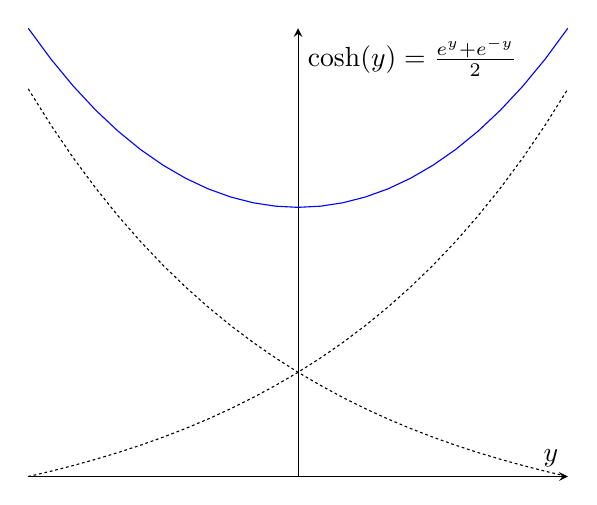
\begin{tikzpicture}
				\begin{axis}[
					axis lines = middle,
					xlabel = $y$,
					ylabel = {$\cosh(y)=\frac{e^y+e^{-y}}{2}$},
					xtick=\empty,
					ytick=\empty,
					legend style={at={(1.5,0.5)},anchor=south east}
					]
					\addplot [
					domain=-1:1, 
					samples y = 0,
					color=blue,
					]
					{cosh(x)};
					\addplot [
					domain=-1:1, 
					samples y = 0, 
					dash pattern=on 1pt off 1pt
					]
					{0.5*e^x};
					\addplot [
					domain=-1:1, 
					samples y = 0, 
					dash pattern=on 1pt off 1pt
					]
					{0.5*e^(-x)};	
				\end{axis}
			\end{tikzpicture}
		\end{center}

		But $\cosh y > 0$, so use $n = 2N$ (always even). So $\cosh y = 1000$, and $y = \pm \cosh^{-1}(1000) \approx \pm 7.6$ (There are two solutions, i.e. note the $\pm$ sign, as the figure above shows). 
	\end{itemize}
	The final answer is that $z = x+ iy = (4N + 1) \dfrac{\pi}{2} \pm i \cosh^{-1}(1000)$
\end{example}
\subsection{Logarithmic Functions}
How to define $\log z$? Let $z = e^w$ and solve for $w$. Note that: \begin{itemize}
	\item exponential function is periodic, so $\log$ will be a ``multi-valued function''
	\item in $\mathbb{C}$, we use ``$\log$'' instead of ``$\ln$''
\end{itemize}
\begin{definition}
	Now, \begin{align*}
		z = e^w &\Rightarrow \; re^{i{\theta + 2\pi k}} = e^{u+iv}\\
		&\Rightarrow \; r = e^u, \;\; \theta + 2\pi k = v\\
		&\Rightarrow \; u = \ln r, \;\; v = \theta + 2\pi k
	\end{align*}
	So, we define \begin{tcolorbox}[hbox, before=\par\smallskip\centering]
		$\log z = \ln |z| + i \arg z$
	\end{tcolorbox}
\end{definition}
\begin{example}
	\begin{itemize}
		\item $\log (1+i) = \ln |1+i| + i\arg (1+i) = \ln \sqrt{2} + i \bigg(\dfrac{\pi}{4} + 2\pi k\bigg)$
		\item $\log(i) = \ln |i| + i\arg (i) = 0 + i \bigg(\dfrac{\pi}{2} + 2\pi k\bigg)$
	\end{itemize}
\end{example}
\begin{proposition}
	We have the following identity: \begin{align*}
		\log(z_1z_2) &= \ln |z_1z_2| + i \arg (z_1z_2)\\
		&=^* \ln |z_1| + \ln |z_2| + i(\arg z_1 + \arg z_2)\\
		&= \log(z_1) + \log(z_2)
	\end{align*}
	Similarly $$\log\bigg(\dfrac{z_1}{z_2}\bigg) =^* \log(z_1) - \log(z_2)$$
	By $=^*$, we actually mean that \underline{the set of values} of $\log(z_1z_2)$ is equal to \underline{the set of values} of $\log(z_1) + \log(z_2)$, due to the multi-valuedness of $\log$. 
\end{proposition}
\begin{definition}
	The \underline{\textbf{principle value of the Logarithm}} is $$\Log(z) = \ln |z| + i \underbrace{\Arg(z)}_{\in (-\pi, \pi] \text{ usually}}$$
\end{definition}
\begin{example}
	\begin{itemize}
		\item $\Log(1+i) = \ln |1+i| + i\Arg (1+i) = \ln \sqrt{2} + i \dfrac{\pi}{4}$
		\item $\Log(i) = \ln |i| + i\Arg (i) = 0 + i \pi$
		\item $\Log e^z = z$ if and only if $Im(z) \in (-\pi, \pi]$
		\item $\Log z$ has discontinuity on negative real axis
		\begin{center}
			\begin{tikzpicture}
				\draw [->,line width=0.8pt] (-6,0) -- (3,0);
				\draw [->,line width=0.8pt] (0,-3) -- (0,3);
				\draw [shift={(0,0)},->,line width=1.2pt] (-180:1.6528925619834707) arc (-180:177.6721849109589:1.6528925619834707);
				\begin{scriptsize}
					\draw [color=black] (0,0) circle (2pt);
					\draw [fill=black] (-5,0) circle (2.5pt);
					\draw [fill=black] (-4.381983471074378,0) circle (2.5pt);
					\draw [fill=black] (-3.6051239669421467,0) circle (2.5pt);
					\draw [fill=black] (-2.84479338842975,0) circle (2.5pt);
					\draw [fill=black] (-2.233223140495866,0) circle (2.5pt);
					\draw [fill=black] (-1.588595041322312,0) circle (2.5pt);
				\end{scriptsize}
			\end{tikzpicture}
		\end{center}
		\item $\Log z$ is analytic everywhere else, with $$\dfrac{d}{dz} \Log z = \dfrac{1}{z}$$
	\end{itemize}
\end{example}
\begin{proof}
	Let \begin{align*}
		w = \Log z &= \ln |z| + i \Arg (z)\\
		&=\dfrac{1}{2} \ln (x^2+y^2) + i \bigg(\arctan (\dfrac{y}{x}) \pm \pi\bigg)\\
		&= u(x,y) + iv(x,y)
	\end{align*}
	Now, \begin{align*}
		\dfrac{dw}{dz} &= \dfrac{\partial u}{\partial x} - i\dfrac{\partial u}{\partial y}\\
		&=\dfrac{x}{x^2+y^2} - i \dfrac{y}{x^2+y^2}\\
		&=\dfrac{x-iy}{x^2+y^2} \cdot \dfrac{x+iy}{x+iy}\\
		&= \dfrac{1}{z}
	\end{align*}
\end{proof}
\begin{definition}
	\underline{\textbf{Branch Cuts}}: Let $f(z)$ be a multivalued function. $F(z)$ is said to be a \underline{\textbf{branch}} of $f(z)$ on a domain $D$ if $F(z)$ is continuous on $D$ and for each $z \in D$, $F(z)$ is one and only one of the values of $f(z)$. 
\end{definition}
\begin{example}
	$\Log z$ is a branch of $\log z$
\end{example}
We could define different branches of $\log z$ by $$\Log_{\tau} z = \ln |z| + i \Arg_{\tau}(z)$$
where $\Arg_{\tau}(z) \in (\tau, \tau + 2\pi]$. Note that $\Log z = \Log_{-\pi}$
\begin{center}
	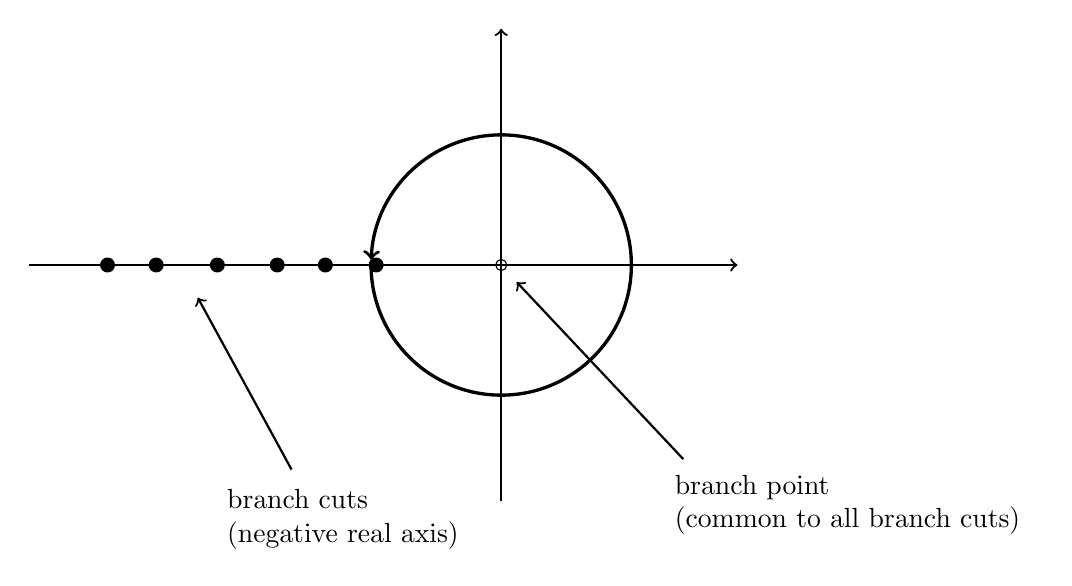
\begin{tikzpicture}
		\draw [->,line width=0.8pt] (-6,0) -- (3,0);
		\draw [->,line width=0.8pt] (0,-3) -- (0,3);
		\draw [shift={(0,0)},->,line width=1.2pt] (-180:1.6528925619834707) arc (-180:177.6721849109589:1.6528925619834707);
		\draw [->,line width=0.8pt] (-2.6629752066115677,-2.5973553719008198) -- (-3.853057851239666,-0.41553719008263945);
		\draw [->,line width=0.8pt] (2.3122314049586783,-2.4651239669421425) -- (0.19652892561983615,-0.21719008264462314);
		\draw (2.080826446280993,-2.5477685950413167) node[anchor=north west] {\parbox{4.570247933884296 cm}{branch point\\(common to all branch cuts)}};
		\draw (-3.6051239669421467,-2.7295867768594984) node[anchor=north west] {\parbox{3.6446280991735533 cm}{branch cuts \\ (negative real axis)}};
		\begin{scriptsize}
			\draw [color=black] (0,0) circle (2pt);
			\draw [fill=black] (-5,0) circle (2.5pt);
			\draw [fill=black] (-4.381983471074378,0) circle (2.5pt);
			\draw [fill=black] (-3.6051239669421467,0) circle (2.5pt);
			\draw [fill=black] (-2.84479338842975,0) circle (2.5pt);
			\draw [fill=black] (-2.233223140495866,0) circle (2.5pt);
			\draw [fill=black] (-1.588595041322312,0) circle (2.5pt);
		\end{scriptsize}
	\end{tikzpicture}
\end{center}
\begin{example}
	$$\Log_{-\frac{\pi}{2}} \ln |z| + i\Arg_{-\frac{\pi}{2}}(z)$$
	\begin{center}
		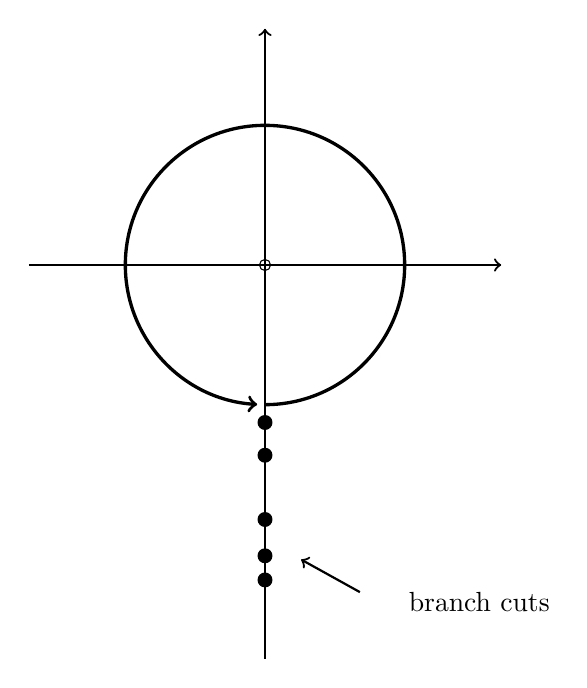
\begin{tikzpicture}
			\draw [->,line width=0.8pt] (-3,0) -- (3,0);
			\draw [->,line width=0.8pt] (0,-5) -- (0,3);
			\draw [shift={(0,0)},->,line width=1.2pt] (-90:1.7738359201773826) arc (-90:266.7698642896959:1.7738359201773826);
			\draw [->,line width=0.8pt] (1.2050433380366845,-4.154259221931055) -- (0.45841564200766105,-3.7405281193307647);
			\draw (1.7017173956863516,-4.030090707518638) node[anchor=north west] {branch cuts};
			\begin{scriptsize}
				\draw [fill=black] (0,-2) circle (2.5pt);
				\draw [color=black] (0,0) circle (2pt);
				\draw [fill=black] (0,-2.4159000201572205) circle (2.5pt);
				\draw [fill=black] (0,-3.231864543438816) circle (2.5pt);
				\draw [fill=black] (0,-3.693061882684935) circle (2.5pt);
				\draw [fill=black] (0,-4) circle (2.5pt);
			\end{scriptsize}
			\end{tikzpicture}
	\end{center}
\end{example}
\begin{example}
	Find a branch of $f(z) = \log(z+4)$ that is analytic at $z = -5$ and equals $7\pi i$ there. 

	\textbf{\underline{Solution}}: We want $\Log_{\tau}(-5+4) = \Log_{\tau}(-1) = 7\pi i$ for some $\tau$.

	So, $\ln|-1| + i\Arg_{\tau}(-1) = 7\pi i$ for some $k$, i.e. $$0 + i\underbrace{(\pi + 2k\pi)}_{\in (\tau, \tau + 2\pi]} = 7\pi i \;\;\text{ for some } k$$ 
	Hence, $k = 3$. We can choose $\tau = 6\pi$ so that $7\pi \in (6\pi, 8\pi]$. 

	The final answer would be $F(z) = \Log_{6\pi}(z+4)$
	\begin{center}
		\begin{tikzpicture}
			\draw [->,line width=0.8pt] (-8,0) -- (7,0);
			\draw [->,line width=0.8pt] (0,-3) -- (0,3);
			\draw [shift={(-5,0)},->,line width=1.2pt] (2.109283615747696:1.9965967101531474) arc (2.109283615747696:359.6393995753092:1.9965967101531474);
			\begin{scriptsize}
				\draw [color=black] (-5,0) circle (2.5pt);
				\draw [color=black] (-1.2227412365286425,-0.02377311401021034) circle (2.5pt);
				\draw [color=black] (-4,0) circle (2.5pt);
				\draw [color=black] (-2,0) circle (2.5pt);
				\draw [color=black] (0,0) circle (2.5pt);
				\draw [color=black] (1,0) circle (2.5pt);
				\draw [color=black] (2,0) circle (2.5pt);
				\draw [color=black] (3,0) circle (2.5pt);
				\draw [color=black] (4,0) circle (2.5pt);
				\draw [color=black] (5,0) circle (2.5pt);
			\end{scriptsize}
		\draw (-5,-0.5) node[anchor=north west] {\large -4};
		\end{tikzpicture}
	\end{center}
\end{example}
\begin{example}
	Where is $f(z) = \Log(z^2+1)$ analytic? 

	\textbf{\underline{Solution}}: We need $z^2+1 \neq 0$ and not equal to negative real number. 

	So, $z^2 +1 = (x+yi)^2+1 = (x^2-y^2+1) + i(2xy)$. 

	$z^2+1 = 0$ when $\begin{dcases}
		x = 0 \text{ and } y = \pm 1\\
		\text{or}\\
		y = 0 \text{ and } x^2+1 = 0 \text{ This is impossible for } x \in \mathbb{R}
	\end{dcases}$

	Hence, $z = \pm i$ here. 

	$z^2+1 < 0$ (real) when $\begin{dcases}
		x = 0 \text{ and } 1-y^2 < 0 & \Rightarrow y^2 > 1 \Rightarrow y > 1 \text{ or } y < -1\\
		\text{or}\\
		y = 0 \text{ and } 1+x^2 < 0 & \text{ Impossible}
	\end{dcases}$

	Hence, $z = iy$ where $|y| > 1$. 
	
	For all other points, $$f'(z) = \dfrac{2z}{z^2+1}$$
	\begin{center}
		\begin{tikzpicture}[scale=0.5]
			\draw (0.5,1) node[anchor=west] {$i$};
			\draw (0.5,-1) node[anchor=west] {$-i$};
			\draw [->,line width=0.8pt] (-3,0) -- (3,0);
			\draw [->,line width=0.8pt] (0,-5) -- (0,5);
			\draw [color=black] (0,-2) circle (2.5pt);
			\draw [color=black] (0,1) circle (2pt);
			\draw [color=black] (0,-1) circle (2pt);
			\draw [color=black] (0,-2) circle (2.5pt);
			\draw [color=black] (0,-3) circle (2.5pt);
			\draw [color=black] (0,-3.6) circle (2.5pt);
			\draw [color=black] (0,-4) circle (2.5pt);
			\draw [color=black] (0,2) circle (2.5pt);
			\draw [color=black] (0,3) circle (2.5pt);
			\draw [color=black] (0,3.6) circle (2.5pt);
			\draw [color=black] (0,4) circle (2.5pt);
		\end{tikzpicture}
	\end{center}
\end{example}

Here is another way to solve the above problem. $$\Log(z^2+1) = \Log((z+i)(z-i)) = \Log_{\tau_1}(z+i) + \Log_{\tau_2}(z-i)$$ for some $\tau_1, \tau_2$

Some possibilities are: \begin{itemize}
	\item $\tau_1 = \dfrac{-\pi}{2}$, $\tau_2 = \dfrac{-3\pi}{2}$
	\item $\tau_1 = \dfrac{3\pi}{2}$, $\tau_2 = \dfrac{-7\pi}{2}$
	\item $\cdots$
	\begin{center}
		\begin{tikzpicture}[scale=0.5]
			\draw [->,line width=0.8pt] (-3,0) -- (3,0);
			\draw [->,line width=0.8pt] (0,-5) -- (0,5);
			\draw [color=black] (0,-2) circle (2.5pt);
			\draw [color=black] (0,1) circle (2pt);
			\draw [color=black] (0,-1) circle (2pt);
			\draw [color=black] (0,-2) circle (2.5pt);
			\draw [color=black] (0,-3) circle (2.5pt);
			\draw [color=black] (0,-3.6) circle (2.5pt);
			\draw [color=black] (0,-4) circle (2.5pt);
			\draw [color=black] (0,2) circle (2.5pt);
			\draw [color=black] (0,3) circle (2.5pt);
			\draw [color=black] (0,3.6) circle (2.5pt);
			\draw [color=black] (0,4) circle (2.5pt);
		\end{tikzpicture}
	\end{center}
\end{itemize}

Finally, note that $$\Log z = \ln |z| + i \Arg z$$ $\Log z$ is analytic, so $\ln |z|$ and $\Arg z$ are harmonic. 

Level curves of $\ln |z| = k$ and $\Arg z = k$ are circles and rays. This would be particularly useful when we deal with temperature problems later. 
\begin{center}
	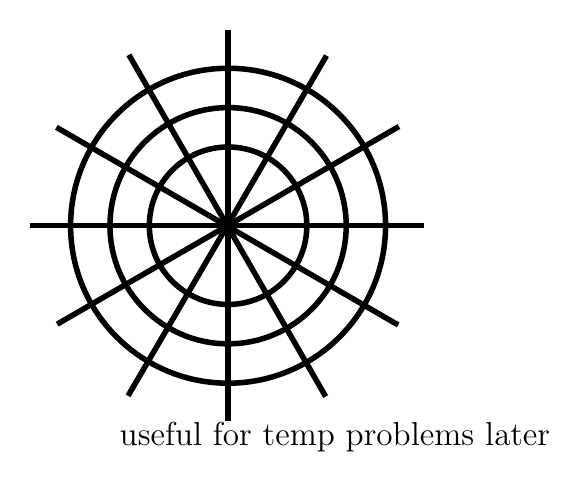
\begin{tikzpicture}[scale=0.5]
		\draw [line width=2pt] (0,0) circle (2.cm);
		\draw [line width=2pt] (0,0) circle (3cm);
		\draw [line width=2pt] (0,0) circle (4cm);
		\draw [line width=2pt] (-2.52,4.34)-- (2.48,-4.34);
		\draw [line width=2pt] (0,-4.96)-- (0,4.96);
		\draw [line width=2pt] (-4.36,2.5)-- (4.32,-2.52);
		\draw [line width=2pt] (-2.54,-4.32)-- (2.5,4.32);
		\draw [line width=2pt] (-5.02,0)-- (4.98,0);
		\draw [line width=2pt] (-4.34,-2.5)-- (4.34,2.52);
		\draw (-3,-6) node[anchor=south west] {\large useful for temp problems later};
	\end{tikzpicture}
\end{center}

\subsection{Complex Powers and Inverse Trigonometric Functions}
\begin{definition}
	\underline{\textbf{Complex Powers}}: We define $$z^\alpha = e^{\alpha \log z} \;\;\; \text{ for } \alpha \in \mathbb{C}, z \neq 0$$ 
\end{definition}
\begin{example}
	\begin{enumerate}
		\item \begin{align*}
			4^{1/2} &= e^{\frac{1}{2}\log 4}\\
			&=e^{\frac{1}{2}(\ln |4| + i \arg (4))}\\
			&=e^{\frac{1}{2}\ln 4 + i \frac{1}{2}(0+2\pi k)}\\
			&=e^{\frac{1}{2}2\ln 2 + i\pi k}\\
			&= e^{\ln 2} e^{i \pi k}\\
			&= 2 \cdot (\pm 1)\\
			&= \pm 2
		\end{align*}
		\item \begin{align*}
			(1+i)^3 &= e^{3 \log (1+i)}\\
			&=e^{3\big(\ln \sqrt{2} + i\arg (1+i)\big)}\\
			&=e^{\frac{3}{2}\ln 2}e^{i 3\big(\frac{\pi}{4}+ 2k\pi\big)}\\
			&=(e^{\ln 2})^{\frac{3}{2}} \cdot \bigg(\cos \dfrac{3\pi}{4} + i \sin \dfrac{3\pi}{4}\bigg)\\
			&=2^{\frac{3}{2}} \cdot \bigg(\dfrac{-1}{\sqrt{2}} + i\dfrac{1}{\sqrt{2}} \bigg)\\
			&=-2+2i
		\end{align*}
		\item \begin{align*}
			i^i &= e^{i \ln |i| + i \arg i}\\
			&=e^{i\big(0 + i (\frac{\pi}{2}+2k\pi)\big)}\\
			&=e^{-\big(\frac{\pi}{2}+2\pi k\big)}\\
			&= \cdots , e^{\frac{-5\pi}{2}}, e^{\frac{-\pi}{2}}, e^{\frac{3\pi}{2}}, \cdots
		\end{align*}
	\end{enumerate}
\end{example}
If we want a single value, take the principal branch to be $e^{\alpha \Log z}$, which is analytic everywhere $\Log z$ is, and $$\dfrac{d}{dz} z^{\alpha} = \dfrac{d}{dz} e^{\alpha \Log z} = e^{\alpha \Log z} \cdot \dfrac{\alpha}{z} = z^\alpha \cdot \dfrac{\alpha}{z} = \alpha z^{\alpha}$$
as expected.
\begin{definition}
	\underline{\textbf{Inverse Trigonometric Functions}}: First, we see that $w = \sin^{-1}z$ means $z = \sin w$, etc. Also, we've accepted multivalued functions. 

	In $\mathbb{R}$, the inverse hyperbolic function can be expressed in terms of logs: \begin{align*}
		y = \sinh x &= \dfrac{1}{2}(e^x - e^{-x})\\
		e^x - 2y -e^{-x} &= 0\\
		(e^x)^2 - 2y(e^x) -1 &= 0 \;\;\;\text{ note that this is a quadratic equation for }e^x\\
		e^x = \dfrac{2y \pm \sqrt{4y^2+4}}{2} &= y \pm \sqrt{y^2+1} \text{ we take the plus sign since } e^x > 0
	\end{align*}
	So, $x = \ln (y + \sqrt{y^2+1}) = \sinh^{-1}y$. 

	In $\mathbb{C}$, we define $\sinh^{-1}z = \log(z + \sqrt{z^2+1})$. 

	Similarly, $\sin^{-1}z = -i \log (iz + (1-z^2)^{\frac{1}{2}})$. Note that for this fefinition, it involves two sets of branches, one with $\log$, and the other one with $(1-z^2)^{\frac{1}{2}}$
\end{definition}
\section{Complex Integration}
\subsection{Contours}
How to integrate in $\mathbb{C}$? 

Complex values functions of a real variable are easy to integrate: $$\int_a^b \bigg(u(t)+iv(t)\bigg)dt = \int_a^b u(t)dt + i \int_a^b v(t)dt$$
\begin{example}
	\begin{enumerate}
		\item $$\int_0^1(t+i)^2 dt \int_0^1 \bigg((t^2-1)+i(2t)\bigg)dt = \dfrac{-2}{3}+2i$$
		\item We can use a special trick (instead of using integration by parts twice). 
		\begin{align*}
			\int_0^\pi e^{2\pi}\cos x dx &= \int_0^\pi e^2x(Re(e^ix))dx\\
			&=Re \bigg(\int_0^\pi e^{(2+i)\pi}\bigg)\\
			&=Re \bigg(\left.\dfrac{e^{(2+i)}}{2+i} \right\vert_{0}^{\pi} \bigg)\\
			&=Re \bigg(\left.\dfrac{e^{2x}(\cos x + i\sin x)}{2+i} \cdot \dfrac{2-i}{2-i}\right\vert_{0}^{\pi}\bigg)\\
			&=\bigg[\left.\dfrac{2}{5}e^{2x}\cos x + \dfrac{1}{5}e^{2x}\sin x \bigg]\right\vert_{0}^{\pi}\\
			&=-\dfrac{2}{5}e^{-2\pi} + \dfrac{2}{5}
		\end{align*}
	\end{enumerate}
\end{example}
What about integrating a function of a complex variable? 

We will replace the intervals with paths.
\begin{definition}
	Let $z(t) = x(t) + iy(t)$ on $t \in [a, b]$ be continuous. The range is a \underline{\textbf{curve}} $\mathcal{C}$, and is called a \textbf{\underline{smooth curve}} if $z'(t)$ is continuous and non-zero on $[a,b]$

	\begin{center}
		\begin{center}
			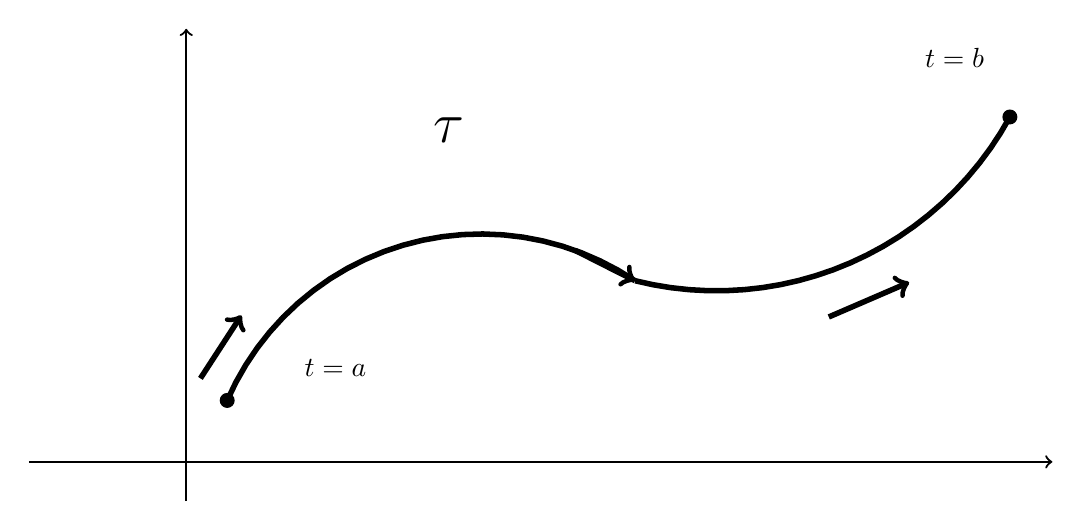
\begin{tikzpicture}
				\draw [->,line width=0.8pt] (-6,-0.5) -- (7,-0.5);
				\draw [->,line width=0.8pt] (-4,-1) -- (-4,5);
				\draw [shift={(-0.25584946236559125,-1.1211182795698924)},line width=2pt]  plot[domain=0.9807967459735268:2.73164434839709,variable=\t]({1*3.5154344145031557*cos(\t r)+0*3.5154344145031557*sin(\t r)},{0*3.5154344145031557*cos(\t r)+1*3.5154344145031557*sin(\t r)});
				\draw [shift={(2.7343127336705524,5.919553551792389)},line width=2pt]  plot[domain=4.466399761960735:5.782317247845397,variable=\t]({1*4.247413836338335*cos(\t r)+0*4.247413836338335*sin(\t r)},{0*4.247413836338335*cos(\t r)+1*4.247413836338335*sin(\t r)});
				\draw [->,line width=2pt] (0.9421669742181896,2.1838833452932853) -- (1.7,1.8);
				\draw [->,line width=2pt] (-3.82,0.56) -- (-3.3,1.36);
				\draw [->,line width=2pt] (4.16,1.34) -- (5.18,1.78);
				\draw (-2.62,0.92) node[anchor=north west] {$t=a$};
				\draw (5.26,4.88) node[anchor=north west] {$t=b$};
				\draw (-0.98,4) node[anchor=north west] {\huge $\tau$};
				\begin{scriptsize}
					\draw [fill=black] (-3.48,0.28) circle (2.5pt);
					\draw [fill=black] (6.46,3.88) circle (2.5pt);
				\end{scriptsize}
				\end{tikzpicture}
		\end{center}
	\end{center}

	A curve is called \textbf{\underline{simple}} if $z(t_1)\neq z(t_2)$ whenever $t_1 \neq t_2$ for $a < t_i < b$ (basically no self intersection)
	
	\begin{center}
		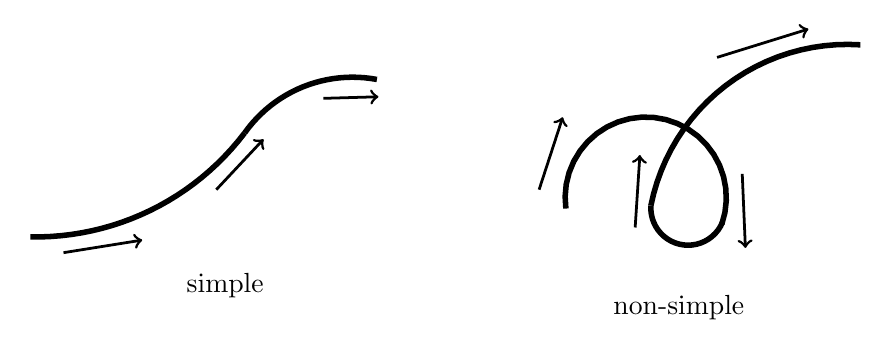
\begin{tikzpicture}
			\draw [shift={(-5.999587628865979,4.0579381443298965)},line width=2pt]  plot[domain=4.6942922471538715:5.634113397410818,variable=\t]({1*3.3384847925306693*cos(\t r)+0*3.3384847925306693*sin(\t r)},{0*3.3384847925306693*cos(\t r)+1*3.3384847925306693*sin(\t r)});
			\draw [shift={(-1.9696,1.0696)},line width=2pt]  plot[domain=1.3853605779174:2.5254415053168207,variable=\t]({1*1.6791879942400734*cos(\t r)+0*1.6791879942400734*sin(\t r)},{0*1.6791879942400734*cos(\t r)+1*1.6791879942400734*sin(\t r)});
			\draw (-4.2,0.38) node[anchor=north west] {simple};
			\draw (1.22,0.1) node[anchor=north west] {non-simple};
			\draw [shift={(1.7541468126207345,1.2190534449452672)},line width=2pt]  plot[domain=-0.3376013374048332:3.2778566866789682,variable=\t]({1*1.0236354908364311*cos(\t r)+0*1.0236354908364311*sin(\t r)},{0*1.0236354908364311*cos(\t r)+1*1.0236354908364311*sin(\t r)});
			\draw [shift={(2.292154717838775,1.0881031452258503)},line width=2pt]  plot[domain=3.074139205941243:5.883297847980803,variable=\t]({1*0.4732309023319334*cos(\t r)+0*0.4732309023319334*sin(\t r)},{0*0.4732309023319334*cos(\t r)+1*0.4732309023319334*sin(\t r)});
			\draw [shift={(4.315807275047862,0.6198787492022976)},line width=2pt]  plot[domain=1.5062464102482258:2.9438273487333233,variable=\t]({1*2.545422404961757*cos(\t r)+0*2.545422404961757*sin(\t r)},{0*2.545422404961757*cos(\t r)+1*2.545422404961757*sin(\t r)});
			\draw [->,line width=1pt] (0.4,1.32) -- (0.7,2.24);
			\draw [->,line width=1pt] (2.98,1.52) -- (3.02,0.58);
			\draw [->,line width=1pt] (2.66,3) -- (3.82,3.36);
			\draw [->,line width=1pt] (1.62,0.84) -- (1.68,1.76);
			\draw [->,line width=1pt] (-5.64,0.52) -- (-4.64,0.68);
			\draw [->,line width=1pt] (-3.7,1.32) -- (-3.1,1.96);
			\draw [->,line width=1pt] (-2.34,2.48) -- (-1.64,2.5);
		\end{tikzpicture}
	\end{center}

	If $z(a) = z(b)$, then the curve is called a \underline{\textbf{closed}} curve. 
	\begin{center}
		\begin{tikzpicture}[line cap=round,line join=round,>=triangle 45,x=1cm,y=1cm, scale=0.5]
			\clip(-8.94,-5.24) rectangle (8.9,5.24);
			\draw (-5.24,-0.1) node[anchor=north west] {simple closed curve};
			\draw [rotate around={-0.5256346064576136:(-3.44,2.18)},line width=2pt] (-3.44,2.18) ellipse (2.561498385867353cm and 1.3447951445484385cm);
			\draw [->,line width=1pt] (-4.24,3.96) -- (-5.3,3.6);
			\draw [->,line width=1pt] (-1.84,0.66) -- (-0.82,1.26);
			\begin{scriptsize}
				\draw [fill=black] (-1.46,3.02) circle (2.5pt);
			\end{scriptsize}
		\end{tikzpicture}
	\end{center}
\end{definition}
\begin{definition}
	\underline{\textbf{Contour}}: a curve that is composed of finitely many smooth curves, joined end-to-end
	\begin{center}
		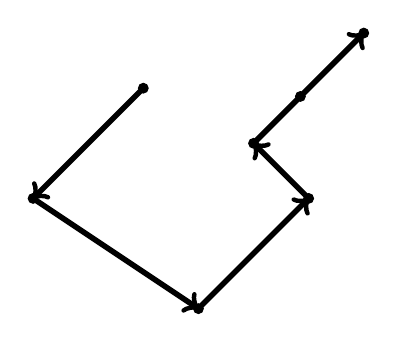
\begin{tikzpicture}[scale=0.7]
			\draw [->,line width=2pt] (-2,3) -- (-4,1);
			\draw [->,line width=2pt] (-4,1) -- (-1,-1);
			\draw [->,line width=2pt] (-1,-1) -- (1,1);
			\draw [->,line width=2pt] (1,1) -- (0,2);
			\draw [->,line width=2pt] (0,2) -- (2,4);
				\draw [fill=black] (-2,3) circle (2.5pt);
				\draw [fill=black] (-4,1) circle (2.5pt);
				\draw [fill=black] (-1,-1) circle (2.5pt);
				\draw [fill=black] (1,1) circle (2.5pt);
				\draw [fill=black] (0,2) circle (2.5pt);
				\draw [fill=black] (2,4) circle (2.5pt);
				\draw [fill=black] (0.85,2.85) circle (2.5pt);
		\end{tikzpicture}
	\end{center}
\end{definition}
\begin{definition}
	\textbf{\underline{Jordan Curve}}: a simple closed contour. 
	\begin{center}
		\begin{tikzpicture}[scale=0.7]
			\draw [line width=2pt] (-3,3)-- (-3,2);
			\draw [line width=2pt] (-3,1)-- (-3,0);
			\draw [line width=2pt] (-3,0)-- (-1,0);
			\draw [line width=2pt] (0,0)-- (2,0);
			\draw [line width=2pt] (-3,3)-- (-1,3);
			\draw [line width=2pt] (0,3)-- (2,3);
			\draw [->,line width=2pt] (-3,2) -- (-3,0.64);
			\draw [->,line width=2pt] (-1,0) -- (0.5,0);
			\draw [->,line width=2pt] (0,3) -- (-1.14,3);
			\draw [shift={(1.974305555555555,1.5)},line width=2pt]  plot[domain=-1.5536683722863849:1.5536683722863849,variable=\t]({1*1.5002200520174724*cos(\t r)+0*1.5002200520174724*sin(\t r)},{0*1.5002200520174724*cos(\t r)+1*1.5002200520174724*sin(\t r)});
			\draw [->,line width=1pt] (3.1,0.04) -- (3.76,0.76);
		\end{tikzpicture}
	\end{center}
\end{definition}
\begin{definition}
	\underline{\textbf{Positively Oriented}}: means its interior lies to the \textbf{\underline{left}} as we follow the curve 
	\begin{center}
		\begin{tikzpicture}[scale=0.7]
			\draw [shift={(-3.6435961272475796,1.366182572614108)},line width=2pt]  plot[domain=-0.1888212477248068:3.7677517930624838,variable=\t]({1*1.2050138375096797*cos(\t r)+0*1.2050138375096797*sin(\t r)},{0*1.2050138375096797*cos(\t r)+1*1.2050138375096797*sin(\t r)});
			\draw [shift={(4.824778887303846,-0.5206419400855922)},line width=2pt]  plot[domain=2.9174621442108837:3.4291939100256186,variable=\t]({1*7.471662137040131*cos(\t r)+0*7.471662137040131*sin(\t r)},{0*7.471662137040131*cos(\t r)+1*7.471662137040131*sin(\t r)});
			\draw [shift={(-1.6738689866939613,-2.4575332650972364)},line width=2pt]  plot[domain=3.4089546984895436:5.468504620115656,variable=\t]({1*0.6906697012568346*cos(\t r)+0*0.6906697012568346*sin(\t r)},{0*0.6906697012568346*cos(\t r)+1*0.6906697012568346*sin(\t r)});
			\draw [shift={(-0.8529559748427671,-3.3321855345911944)},line width=2pt]  plot[domain=-1.505989538730427:2.3212525496456813,variable=\t]({1*0.5088827247571559*cos(\t r)+0*0.5088827247571559*sin(\t r)},{0*0.5088827247571559*cos(\t r)+1*0.5088827247571559*sin(\t r)});
			\draw [shift={(-5.662695492180313,0.6421803127874881)},line width=2pt]  plot[domain=-1.6065757282617978:0.01708835685192156,variable=\t]({1*1.0428477504724725*cos(\t r)+0*1.0428477504724725*sin(\t r)},{0*1.0428477504724725*cos(\t r)+1*1.0428477504724725*sin(\t r)});
			\draw [shift={(-5.904015080113101,-1.1005466540999058)},line width=2pt]  plot[domain=1.2874114365651281:4.105741421103375,variable=\t]({1*0.7296490714611567*cos(\t r)+0*0.7296490714611567*sin(\t r)},{0*0.7296490714611567*cos(\t r)+1*0.7296490714611567*sin(\t r)});
			\draw [shift={(2.164636519748135,11.968551803091001)},line width=2pt]  plot[domain=4.156857863606362:4.525786580780108,variable=\t]({1*16.087832833107946*cos(\t r)+0*16.087832833107946*sin(\t r)},{0*16.087832833107946*cos(\t r)+1*16.087832833107946*sin(\t r)});
			\draw [->,line width=1pt] (-2.18,-1.32) -- (-2.18,-0.38);
			\draw [->,line width=1pt] (-3.08,2.86) -- (-4.18,2.88);
			\draw [->,line width=1pt] (-5.26,2.08) -- (-5.32,1.2);
			\draw [->,line width=1pt] (-5.9,-0.06) -- (-7.06,-0.36);
			\draw [->,line width=1pt] (-6.38,-2.1) -- (-5.46,-2.78);
			\draw [->,line width=1pt] (-0.04,-4.04) -- (0.28,-3.04);
		\end{tikzpicture}
	\end{center}
\end{definition}

\begin{example}
	Parameterize this: 
	\begin{center}
		\begin{tikzpicture}
			\draw [->,line width=2pt] (-3,0) -- (6,0);
			\draw [->,line width=2pt] (1,-1) -- (1,4);
			\draw [line width=2pt] (-1,1)-- (3,1);
			\draw [line width=2pt] (3,1)-- (5,3);
			\draw [->,line width=1pt] (-1,1) -- (0,1);
			\draw [->,line width=1pt] (3,1) -- (4,2);
			\draw [->,line width=1pt] (0,1) -- (2.2,1);
			\draw (0.52,1.9) node[anchor=north west] {$i$};
			\draw (0.38,3.3) node[anchor=north west] {$2i$};
			\draw (-1.46,0.02) node[anchor=north west] {$-1$};
			\draw (2.82,0.02) node[anchor=north west] {$1$};
			\draw (4.84,0.02) node[anchor=north west] {$2$};
			\begin{scriptsize}
				\draw [fill=black] (-1,1) circle (2.5pt);
				\draw [fill=black] (3,1) circle (2.5pt);
				\draw [fill=black] (5,3) circle (2.5pt);
			\end{scriptsize}
		\end{tikzpicture}
	\end{center}

	\underline{\textbf{Solution}}: Line segment from $z_0$ to $z_1$ can be parameterized as: $z(t) = z_0 + (z_1 - z_0)t, t \in [0, 1]$. 
	
	For the first curve, \begin{align*}
		z_1(t) &= (-1+i) + (1+i-(-1+i))t\\
		&=-1+i+2t, \;\;\;\; t \in [0,1]
	\end{align*}
	For the second curve, \begin{align*}
		z_2(t) &= (1+i) + (2+2i-(1+i))t\\
		&=1+i+(1+i)t, \;\;\;\; t \in [0,1]
	\end{align*}
	Put everything together we get $$z(t) = \begin{dcases}
		-1+i+2t & t \in [0,1)\\
		1+i+(1+i)(t-1) & t \in [1,2]
	\end{dcases}$$
\end{example}
\begin{example}
	Let $\mathcal{C}$ be a unit circle centered at 0.
	\begin{center}
		\begin{tikzpicture}[scale=0.5]
			\draw [line width=2pt] (0,0) circle (3cm);
			\draw [->,line width=2pt] (-4,0) -- (4,0);
			\draw [->,line width=2pt] (0,-4) -- (0,4);
			\draw [->,line width=1pt] (2.88,2.36) -- (2.22,3.08);
			\draw [->,line width=1pt] (-1.72,3.06) -- (-2.66,2.44);
			\draw [->,line width=1pt] (-3.26,-1.12) -- (-2.76,-1.82);
			\draw [->,line width=1pt] (2.46,-2.56) -- (3.22,-1.58);
			\draw (3.4174,1.4174) node[anchor=north west] {$t=0$};
			\draw (3.3514,-0.1886) node[anchor=north west] {$t=2\pi$};
		\end{tikzpicture}
	\end{center}

	\textbf{\underline{Solution}}: $\mathcal{C}: z(t) = e^{it} \;\;\; t \in [0, 2\pi]$
\end{example}
\begin{example}
	Circle, radius $r_0$, centered at $z_0$? 

	\textbf{\underline{Solution}}: $\mathcal{C}: z(t) = z_0 + r_0e^{it} \;\;\; t \in [0, 2\pi]$
\end{example}
\begin{example}
	Parameterize $y = f(x), x\in [a,b]$

	\textbf{\underline{Solution}}: just let $x(t) = t$, $$z(t) = x(t)+ iy(t) = t + if(t), \;\;\; t \in [a,b]$$
	For example, $y = x^2$ will be parameterized as $z(t) = t + it^2$
\end{example}
\begin{definition}
	\label{defn_Arclength}
	\underline{\textbf{Arclength}}: We define the arclength as follows: 
	\begin{center}
		\begin{tikzpicture}
			\draw [shift={(-5.767313432835821,0.2476119402985072)},line width=2pt]  plot[domain=0.7686526640717644:2.901124440109067,variable=\t]({1*2.3194243549602365*cos(\t r)+0*2.3194243549602365*sin(\t r)},{0*2.3194243549602365*cos(\t r)+1*2.3194243549602365*sin(\t r)});
			\draw [shift={(0.31600561272216865,5.379672591206732)},line width=2pt]  plot[domain=3.814517728837391:4.5170648131457805,variable=\t]({1*5.647052392256123*cos(\t r)+0*5.647052392256123*sin(\t r)},{0*5.647052392256123*cos(\t r)+1*5.647052392256123*sin(\t r)});
			\draw [->,line width=1pt] (-7.7,2.16) -- (-6.9,2.92);
			\draw [->,line width=1pt] (-5.52,2.9) -- (-4.62,2.62);
			\draw [->,line width=1pt] (0.84,0.82) -- (1.4,1.58);
			\draw [->,line width=1pt] (-2.22,1.12) -- (-1.32,0.72);
			\draw [shift={(-0.4598988439306359,2.4977745664739888)},line width=2pt]  plot[domain=4.592526772792368:6.0426280107639405,variable=\t]({1*2.676981583110527*cos(\t r)+0*2.676981583110527*sin(\t r)},{0*2.676981583110527*cos(\t r)+1*2.676981583110527*sin(\t r)});
			\draw [line width=2pt] (-4.1,1.86)-- (-4.1,0.78);
			\draw [line width=2pt] (-4.1,0.78)-- (-2.96,0.78);
			\draw [<->,line width=1pt] (-3.84,2.04) -- (-2.78,1);
			\draw (-9.32,1.4) node[anchor=north west] {$t=a$};
			\draw (2.66,2.24) node[anchor=north west] {$t=b$};
			\draw (-3.86,0.7) node[anchor=north west] {$\Delta{x}$};
			\draw (-5,1.7) node[anchor=north west] {$\Delta{y}$};
			\draw (-3.24,2) node[anchor=north west] {$\Delta s$};
			\draw (-0.02,2.44) node[anchor=north west] {$\Gamma$};
			\begin{scriptsize}
				\draw [fill=black] (-8.02,0.8) circle (2.5pt);
				\draw [fill=black] (-6.58,2.42) circle (2.5pt);
				\draw [fill=black] (-4.1,1.86) circle (2.5pt);
				\draw [fill=black] (-2.96,0.78) circle (2.5pt);
				\draw [fill=black] (0.1,-0.12) circle (2.5pt);
				\draw [fill=black] (2.14,1.86) circle (2.5pt);
				\draw [fill=black] (-4.1,0.78) circle (2.5pt);
			\end{scriptsize}
		\end{tikzpicture}
	\end{center}
	
	Partition the curve \begin{align*}
		\Delta s &\approx \sqrt{\Delta x^2 + \Delta y^2}\\
		&= \sqrt{\bigg(\dfrac{\Delta x}{\Delta t}\bigg)^2 + \bigg(\dfrac{\Delta y}{\Delta t}\bigg)^2} \Delta t
	\end{align*}
	Sum all pieces and let $\Delta t \rightarrow 0$ (Performing a Riemann Sum there): 
	\begin{align*}
		L = \int_R ds &= \int_a^b \sqrt{\bigg(\dfrac{dx}{dt}\bigg)^2+\bigg(\dfrac{dy}{dt}\bigg)^2} dt\\
		&=\int_a^b \left|\dfrac{dz}{dt}\right| dt \;\;\text{ we use modulus here}
	\end{align*}
	The physical interpretation could be: $\text{total\_distance} = \int_a^b (\text{speed})\;dt$
\end{definition}
Now we are ready to integrate $f(z)$ along a curve. 

\subsection{Contour Integrals}
Partition curve $\mathcal{C}$ as shown. Sum, and let $\max |\Delta z_k| \rightarrow 0$: $$\int_{\mathcal{C}}f(z)dz = \lim_{\max |\Delta z_k| \rightarrow 0} \sum_{k} f(z_k^*)\Delta z_k$$
See the text for more detail.

If $\mathcal{C}$ is a single point, define $\int_{\mathcal{C}}f(z)dz = 0$. 

How to calculate? 
\begin{definition}
	Assume $\mathcal{C}$ has a parameterization. Call it $z(t), t \in [a,b]$. Then: \begin{align*}
		\int_{\mathcal{C}} f(z)dz &= \lim_{\max |\Delta z_k| \rightarrow 0} \sum_{k} f(z_k^*) \dfrac{\overbrace{z(t_k)}^{z_k} - \overbrace{z(t_{k-1})}^{z_{k-1}}}{\Delta t_k} \Delta t_k\\
		&= \int_{a}^{b} f(z)z'(t) dt
	\end{align*}
\end{definition}
\begin{proposition}
	Properties: \begin{itemize}
		\item $\int_{\mathcal{C}} \bigg(f(z) +g(z) \bigg)dz = \int_{\mathcal{C}} f(z)dz + \int_{\mathcal{C}} g(z)dz$
		\item $\int_{\mathcal{C}} kf(z)dz = k\int_{\mathcal{C}} f(z)dz$
		\item $\int_{-\mathcal{C}} f(z)dz = -\int_{\mathcal{C}} f(z)dz$. Here $-\mathcal{C}$ means $\mathcal{C}$ traversed in the opposite direction
		\item $\int_{\mathcal{C}_1 + \mathcal{C}_2} f(z)dz = \int_{\mathcal{C}_1} f(z)dz + \int_{\mathcal{C}_2} f(z)dz$. Here it means that we traverse $\mathcal{C}_1$ then traverse $\mathcal{C}_2$. 
	\end{itemize}
\end{proposition}

Is there a triangle inequality? i.e. $$\left| \int_{\mathcal{C}} f(z)dz \right| \leq_? \int_{\mathcal{C}} \left| f(z) \right| dz$$

No! LHS is real, but RHS is complex. ``$\leq$'' does NOT make any sense here. 

\begin{proposition}
	\underline{\textbf{The ``ML'' Inequality}}: If $f(z)$ is continuous on a contour $\mathcal{C}$, then $$\left| \int_{\mathcal{C}} f(z)dz \right| \leq ML$$
	where $M$ is an upper bound for $|f(z)|$ on $\mathcal{C}$ and $L$ is the length of $\mathcal{C}$. 
\end{proposition}
\begin{proof}
	Let $z(t)$, $t \in [a,b]$ be a parameterization of $\mathcal{C}$. Then \begin{align*}
		\left| \int_{\mathcal{C}} f(z)dz \right| &= \left| \int_{a}^b f(z(t))z'(t) dt\right|\\
		&\leq \int_{a}^b \bigg|f(z(t))z'(t)\bigg| dt \;\;\text{ by triangle inequality for integrals w.s.t. real variables}\\
		&= M \int_{a}^b \bigg| z'(t)\bigg| dt\\
		&= ML
	\end{align*}
	Second last step: since $|f(z)| \leq M$ on $\mathcal{C}$. 

	Last step: from last lecture. See Definition \ref{defn_Arclength}.
\end{proof}
\begin{example}
	Find an upper bound on $\left| \int_{\mathcal{C}} e^{\frac{1}{z}}\right|$

	\underline{\textbf{Solution}}: $M = ?$\begin{align*}
		\left| e^{\frac{1}{z}} \right| &= \left| e^{\frac{1}{x+iy}} \right|\\
		&=\left| e^{\frac{x-iy}{x^2+y^2}} \right|\\
		&=\left| e^{\frac{x}{x^2+y^2}} \cdot e^{-i \frac{y}{x^2+y^2}}\right|\\
		&\leq e^{\frac{x}{1}} \;\;\text{ since }x^2+y^2 = 1\\
		&\leq e^1 \;\; \text{ since } x \leq 1
	\end{align*}
	Clearly, $L = 2\pi$, so $\left| e^{\frac{1}{z}} \right| \leq e^1 \cdot 2\pi = 2\pi e$ by ML inequality. 
\end{example}
\begin{example}
	Evaluate $\int_{\mathcal{C}} \cos z dz$ where $\mathcal{C}$ is the line segment from 0 to 1+2i. 

	\textbf{\underline{Solution}}: Parameterize $\mathcal{C}$ by $$z(t) = 0+(1+2i-0)t, \;\;\; t \in [0,1]$$
	Then $$\int_{\mathcal{C}} \cos z dx = \int_{0}^{1} \underbrace{\cos \bigg( (1+2i)t\bigg)}_{f(z(t))}\cdot \underbrace{(1+2i)}_{z'(t)} dt = \left. \sin \bigg( (1+2i)t\bigg) \right|_{0}^{1} = \sin(1+2i) - 0 = \sin(1+2i)$$
\end{example}
\begin{example}
	Evaluate $\int_{\mathcal{C}} \cos z dz$ where $\mathcal{C}$ is: 

	\textbf{\underline{Solution}}: $\mathcal{C} = \mathcal{C}_1 \cup \mathcal{C}_2$ where $\begin{dcases}
		C_1: & z(t) = t, \;\; t\in [0,1)\\
		C_2: & z(t) = 1+(t-1)i, \;\; t \in [1,3]
	\end{dcases}$. So \begin{align*}
		\int_{\mathcal{C}} \cos z dx &= \int_{\mathcal{C}_1} \cos z dx + \int_{\mathcal{C}_2} \cos z dx\\
		&=\int_{0}^1 \cos t dt + \int_{1}^3 \cos (1+(t-1)i) i dt\\
		&= \left. \sin t \right|_0^1 + \left. \sin (1+(t-1)i) \right|_1^3\\
		&= \sin (1) + (\sin (1+2i) - \sin (1))\\
		&= \sin (1+2i)
	\end{align*}
	As before
\end{example}
\begin{example}
	Evaluate $\int_{\mathcal{C}} e^z dz$ where $\mathcal{C}$ is part of $y = x^2 + 1$ from $z = i$ to $z = 2+5i$. 

	\textbf{\underline{Solution}}: Let $z(t) = \underbrace{t}_x + \underbrace{(t^2+1)}_y i, \;\; t \in [0,2]$. Then, \begin{align*}
		\int_{\mathcal{C}} e^z dz &= \int_{0}^{2} e^{z(t)} z'(t) dt\\
		&= \int_{0}^{2} e^{t^2+(t^2+1)i} (1+2ti) dt\\
		&= \left. e^{t^2+(t^2+1)i} \right |_0^2\\
		&= e^{2+5i} - e^i\\
		&= e^z \big|_i^{2+5i}
	\end{align*}
\end{example}
Does it always work that way? See the following example
\begin{example}
	Evaluate $\int_{\mathcal{C}} \overline{z} dz$ where \begin{enumerate}
		\item $\mathcal{C}$ is line segment from 0 to $1+i$
		\item $\mathcal{C}$ is the smallest arc of circle $x^2+(y-1)^2 = 1$ from 0 to $1+i$
	\end{enumerate}

	\textbf{\underline{Solution}}: \begin{enumerate}
		\item parameterization: $z(t) = t(1+i), \;\; t \in [0,1]$
		
		\begin{align*}
			\int_{\mathcal{C}} \overline{z} dz &= \int_{0}^1 t(1-i)\cdot (1+i) dt\\
			&= \int_0^1 2t dt\\
			&=1
		\end{align*}
		\item parameterization: $z(t) = e^{it} + i, \;\; t \in [\dfrac{-\pi}{2},0]$. It's the unit circle, shifted up by 1 unit. 
		
		\begin{align*}
			\int_{\mathcal{C}} \overline{z} dz &= \int_{-\pi / 2}^0 (e^{-it} - i) (ie^{it}) dt\\
			&= \cdots\\
			&= 1+i(\frac{\pi}{2} - 1) dt\\
			&\neq 1
		\end{align*}
	\end{enumerate}
	So, the general answer is no. Different paths might yield different results. 
\end{example}
\subsection{Independence of Path}
\begin{theorem}
	\label{theorem_FTC}
	\underline{\textbf{Complex Extension of Fundamental Theorem of Calculus}}: 

	If $f(z)$ is continuous in a domain $D$ and has antiderivative $F(z)$ throughout $D$, then, for any contour $\mathcal{C}$ lying in $D$ with initial point $z_1$ and terminal point $z_2$, we have $$\int_{\mathcal{C}} f(z) dz = F(z_2) - F(z_1)$$
\end{theorem}
\begin{proof}
	First, suppose $\mathcal{C}$ is smooth, i.e. $z'(t) \neq 0$, continuous. 

	Parameterize by $z(t), t \in [a,b]$. Then, \begin{align*}
		\int_{\mathcal{C}} f(z) dz &= \int_a^b f(z(t))z'(t) dt\\
		&=\int_{\mathcal{C}} \dfrac{d}{dt} \bigg(F\big(z(t)\big)\bigg) dt \;\; \text{ by chain rule}\\
		&=F(z(t)) \bigg|_{t=a}^b\\
		&=F(z(b)) - F(z(a))\\
		&=F(z_2) - F(z_1)
	\end{align*}
	Next, if $\mathcal{C}$ is not smooth, it has a finite number of smooth pieces, since it's a contour. 

	Apply the result above to each piece: \begin{align*}
		\int_{\mathcal{C}} f(z) dz &= \int_{\mathcal{C}_1} f(z) dz + \cdots + \int_{\mathcal{C}_n} f(z) dz\\
		&=\bigg(F(a_1) - F(a_0)\bigg) + \bigg(F(a_2) - F(a_1)\bigg) + \cdots + \bigg(F(a_n) - F(a_{n-1})\bigg) \\
		&=F(a_n) - F(a_0)\\
		&= F(z_2) - F(z_1)
	\end{align*}
\end{proof}
\begin{example}
	Evaluate $\int_{\mathcal{C}}(1+z^2) dz$ where $\mathcal{C}$ is: 

	\textbf{\underline{Solution}}: \begin{align*}
		\int_{\mathcal{C}}(1+z^2) dz &= \left. \left( z + \dfrac{z^3}{4}\right) \right|_{z=0}^{z=4+2i}\\
		&= \cdots\\
		&= \dfrac{28}{3} + \dfrac{94}{3}i
	\end{align*}
\end{example}
\begin{example}
	Evaluate $\int_{\mathcal{C}}e^z dz$ where $\mathcal{C}$ is: 

	\textbf{\underline{Solution}}: \begin{align*}
		\int_{\mathcal{C}}(1+z^2) dz &= e^z \big|_{z=1-i}^{z=1-i}\\
		&= e^{1-i} - e^{1-i}\\
		&= 0
	\end{align*}
\end{example}
\begin{theorem}
	Let $f$ be a continuous function in a domain $D$. Then, the following statements are equivalent: \begin{enumerate}
		\item $f$ has an antiderivative in $D$.
		\item If $\mathcal{C}$ is any closed contour in $D$, then $\int_{\mathcal{C}}f(z) dz = 0$.
		\item The contour integrals of $f$ are independent of path in $D$. 
	\end{enumerate}
\end{theorem}
\begin{proof}
	1 $\Rightarrow$ 2: It follows immediately from Theorem \ref{theorem_FTC} with $\mathcal{C}$ being a closed contour. 

	2 $\Rightarrow$ 3: Let $\mathcal{C}_1$ and $\mathcal{C}_2$ be any two contours in $D$ with same end points. Let $\mathcal{C}$ be the closed contour $\mathcal{C}_1 + (-\mathcal{C}_2)$. 
	
	Then, $\int_{\mathcal{C}}f(z)dz = 0$. So $\int_{\mathcal{C}_1}f(z)dz + \int_{-\mathcal{C}_2}f(z)dz = 0$. So $\int_{\mathcal{C}_1}f(z)dz - \int_{\mathcal{C}_2}f(z)dz = 0$, implying that $$\int_{\mathcal{C}_1}f(z)dz = \int_{\mathcal{C}_2}f(z)dz $$

	3 $\Rightarrow$ 1: Construct the antiderivative. Choose a point $z_0 \in D$, and let $\mathcal{C}$ be the contour as shown. Recall the $D$ is a connected set. 

	Define $F(z) = \int_{\mathcal{C}} f(w) dw$. By 3, $F(z)$ is single valued; We will show that $F'(z) = f(z)$. 

	For any point $z$, choose $\Delta z$ small enough such that the line segment $\Gamma$ parameterized by $$z(t) = z + t \Delta z, \;\; t \in [0,1]$$
	is in $D$ (This is possible since $D$ is open)

	Then \begin{align*}
		F(z + \Delta z) - F(z) &= \left(\int_{\mathcal{C}} f(w) dw + \int_{\Gamma} f(w) dw \right) - \int_{\mathcal{C}} f(w) dw \\
		&= \int_{\Gamma} f(w) dw\\
		&= \int_{0}^1 f(z(t))z'(t) dt\\
		&= \int_{0}^1 f(z+t\Delta z) (\Delta z) dt\\
		\Rightarrow \; \dfrac{F(z + \Delta z) - F(z)}{\Delta z}\;&= \int_{0}^1 f(z+t\Delta z) dt
	\end{align*}
	Let $\Delta z \rightarrow 0$. $$F'(z) = \int_{0}^1 f(z) dt = f(z)\int_{0}^1 dt = f(z)$$
\end{proof}
We showed that $\overline{z}$ can be integreated, but the result depends on path. So $\overline{z}$ is integrable, but not anti-differentiable. Also, functions with antiderivatives are easy; for those without, we must parameterize. 
\subsection{Cauchy's Integral Theorem}
\begin{example}
	\label{example_unit_circle}
	\textbf{Most Important Example in this Course}: Evaluate $\int_{\mathcal{C}} \dfrac{1}{z} dz$ where $\mathcal{C}$ is the unit circle. 

	\textbf{\underline{Solution}}: $\dfrac{1}{z}$ does not have antiderivative over all of $\mathcal{C}$. Any branch of $\log z$ will have a problem, i.e. $\mathcal{C}$ will cross a branch cut. 

	Method 1: Parameterize $\mathcal{C}$ by $e^{it}, t \in [0,2\pi]$. By definition, $$\int_{\mathcal{C}} \dfrac{1}{z} dz = \int_{0}^{2\pi} \dfrac{1}{e^{it}} \cdot i e^{it} dt = 2\pi i$$
	Method 2: Split $\mathcal{C}$ in two, and use Theorem \ref{theorem_FTC} on each. \begin{align*}
		\int_{\mathcal{C}_1} \dfrac{1}{z} dz &= \Log z \big|_{-i}^i \;\; \text{ branch cut at }\theta = -\pi\\
		&= \Log i - \Log (-i)\\
		&= i \dfrac{\pi}{2} - i \left(\dfrac{-\pi}{2}\right)\\
		&=\pi i\\
		\int_{\mathcal{C}_2} \dfrac{1}{z} dz &= \Log_0 z \big|_{i}^{-i}\\
		&= \Log_0 (-i) - \Log_0(i)\\
		&= \dfrac{3\pi}{2}i - \dfrac{\pi}{2}i\\
		&= \pi i
	\end{align*}
	Therefore, $$\int_{\mathcal{C}} \dfrac{1}{z} dz = \int_{\mathcal{C}_1} \dfrac{1}{z} dz + \int_{\mathcal{C}_2} \dfrac{1}{z} dz = \pi i + \pi i = 2\pi i$$
	Go around the contour twice, what's the result? It would be $4\pi i$. Also, going counter-clockwise would yield the result $-2\pi i$
\end{example}
\begin{definition}
	A closed contour $\mathcal{C}$ is said to be \textbf{\underline{continuously deformable}} to a contour $\mathcal{C}_1$ in a domain $D$ if there exists a function $z(s,t)$, continuous for $s \in [0,1], t\in [0,1]$, such that \begin{enumerate}
		\item $z(s,t)$ is a closed contour in $D$ for each $s \in [0,1]$
		\item $z(0,t)$ is a parameterization of $\mathcal{C}$
		\item $z(1,t)$ is a parameterization of $\mathcal{C}_1$
	\end{enumerate}
\end{definition}
\begin{theorem}
	\label{theorem_DIT}
	\underline{\textbf{Deformation Invariance Theorem}}: Let $f$ be analytic in a domain $D$, containing closed contours $\mathcal{C}_1$ and $\mathcal{C}_2$. If $\mathcal{C}_1$ can be continuously deformed into $\mathcal{C}_2$, then $$\int_{\mathcal{C}_1}f(z)dz = \int_{\mathcal{C}_2}f(z)dz$$
\end{theorem}
\begin{proof}
	It's too hard - 12 pages long in one text. 
\end{proof}
\begin{definition}
	A \underline{\textbf{simply connected domain}} is a domain in which every ``loop'' (closed contour) in $D$ can be continuously deformed to a point (while remaining in $D$). 
\end{definition}
\begin{theorem}
	\underline{\textbf{Cauchy's Integral Theorem (Cauchy-Goursat Theorem)}}: 

	If $f$ is analytic in a simply connected domain $D$, and $\mathcal{C}$ is a closed contour in $D$, then $$\int_{\mathcal{C}}f(z)dz = 0$$
\end{theorem}
\begin{proof}
	Follows from Theorem \ref{theorem_DIT} by shrinking $\mathcal{C}$ continuously to a point.
\end{proof}
\begin{corollary}
	Since $\int_{\mathcal{C}}f(z)dz = 0 \Leftrightarrow f$ has an antiderivative in $D$, we have that if $f$ is analytic, then $f$ also has an antiderivative, which is analytic. So every analytic function is infinitely antidifferentiable.  
\end{corollary}
\begin{example}
	Back to Example \ref{example_unit_circle}. We know that $\int_{\mathcal{C}} \dfrac{1}{z}dz = 2\pi i$ for \underline{any} closed contour enclosing the origin. 

	Also, $\int_{\mathcal{C}} \dfrac{1}{z}dz = 0$ for any closed contours \underline{not} enclosing the origin. 

	Could shift results: $$\int_{\mathcal{C}}\dfrac{1}{z-z_0}dz = \begin{dcases}
		0 & \text{ if } z_0 \text{ is exterior to }\mathcal{C}\\
		2\pi i & \text{ if } z_0 \text{ is interior to }\mathcal{C}
	\end{dcases}$$
\end{example}
\end{document}
